\documentclass[aspectratio=43]{beamer}
\usepackage{amsfonts,amsmath,oldgerm}
\usepackage{bm}
\usepackage{siunitx}       % typesetting values with units
\usepackage[ruled]{algorithm2e}
\usepackage{booktabs}       % professional-quality tables
\usepackage{multirow}
\usepackage{subcaption}

% color gradient bar
\usepackage{tikz}
\usepackage{tabularx}

\graphicspath{{Figures/}}  % Location of the graphics files (set up for graphics to be in PDF format)


%algorithm2e
%%% Coloring the comment as blue
\newcommand\mycommfont[1]{\footnotesize\ttfamily\textcolor{blue}{#1}}
\SetCommentSty{mycommfont}

\SetKwInput{KwInput}{\small{Input}}                % Set the Input
\SetKwInput{KwOutput}{\small{Output}}              % set the Output
\SetKwInput{KwData}{\small{Data}}              % set the Output

%tikz
\usetikzlibrary{arrows,positioning} 
\tikzset{
    %Define standard arrow tip
    >=stealth',
    %Define style for boxes
    punkt/.style={
           rectangle,
           rounded corners,
           draw=black, very thick,
           text width=6.5em,
           minimum height=2em,
           text centered},
    % Define arrow style
    pil/.style={
           ->,
           thick,
           shorten <=2pt,
           shorten >=2pt,}
}
\usetikzlibrary{calc}
%Tikz picture
% Input layer neurons'number
\newcommand{\inputnum}{2} 
 
% Hidden layer neurons'number
\newcommand{\hiddennum}{2}  

% Hidden layer neurons'number hard sharing
\newcommand{\hiddennumhs}{4}  

% Hidden layer neurons'number hard sharing
\newcommand{\hiddennumsp}{3}  
 
% Output layer neurons'number
\newcommand{\outputnum}{2} 

% Min Node size
\newcommand{\minnodesize}{5mm} 

\usetheme{sintef}

\newtheorem{proposition}[theorem]{Proposicion}

\newcommand{\testcolor}[1]{\colorbox{#1}{\textcolor{#1}{test}}~\texttt{#1}}

\newcommand\Mark[2][8.4]{%
  \rlap{\tikz[baseline=(current bounding box.south)]{
        \shade[left color=darkgray, right color=maincolor!#2!darkgray]
               (0,0) rectangle ++(#1*#2/100,0.3);}%
  }%
}

% My definitions

  % Math Operators
  \DeclareMathOperator*{\argmin}{arg\min}
  \DeclareMathOperator*{\argmax}{arg\max}
  \DeclareMathOperator*{\arginf}{arg\inf}
  \DeclareMathOperator*{\argsup}{arg\sup}
  \DeclareMathOperator{\Tr}{tr}
  \DeclareMathOperator{\Span}{span}
  \DeclareMathOperator{\Diag}{diag}
  \DeclareMathOperator{\rank}{rank}
  \DeclareMathOperator{\sign}{sign}
  \DeclareMathOperator{\expect}{E}
  \DeclareMathOperator{\VCdim}{VCdim}
  
  \DeclareMathOperator{\mn}{\mathcal{M_N}}
  \DeclareMathOperator{\tn}{\mathcal{T_N}}
  
  
  
  \DeclareMathOperator{\Ima}{Im}
  \DeclareMathOperator{\Ker}{Ker}
  \DeclareMathOperator{\Vector}{vec}
  
%   \DeclarePairedDelimiter\floor{\lfloor}{\rfloor}
%   \DeclarePairedDelimiter\ceil{\lceil}{\rceil}
%   \DeclarePairedDelimiter\equivclass{\lbrack}{\rbrack}
  
  
  
  \newcommand{\comm}[1]{{\color{red} #1}}
  
  \newcommand{\norm}[1]{\left\lVert#1\right\rVert}
  \newcommand{\abs}[1]{\left|#1\right|}
  \newcommand{\mymax}[1]{\max\left(#1\right)}
  \newcommand{\mymin}[1]{\min\left(#1\right)}
  \newcommand{\pospart}[1]{\left[#1\right]_{+}}
  \newcommand{\epsins}[1]{\left[#1\right]_{\epsilon}}
  
  \newcommand{\set}[1]{\left\{#1\right\}}
  \newcommand{\cardinal}[1]{\left|#1\right|}
  \newcommand{\defeq}{\vcentcolon=}
  \newcommand{\hypf}{h}
  \newcommand{\hypfun}[1]{\hypf\left(#1\right)}
  \newcommand{\hyp}[2]{\hypf\left(#1, #2\right)}
  \newcommand{\fun}[1]{f\left(#1\right)}
  \newcommand{\den}[1]{p\left( #1 \right)}
  \newcommand{\opt}[1]{{#1}^*}
  \newcommand{\cond}[2]{P\left( #1 \;\middle\vert\; #2 \right)}
  \newcommand{\normal}[1]{N \left(#1\right)}
  \newcommand{\multinormal}[1]{\mn \left(#1\right)}
  \newcommand{\tensornormal}[1]{\tn \left(#1\right)}
  \newcommand{\tendsto}[2]{\xrightarrow[#1]{} #2}
  \newcommand{\diffp}[2]{\frac{\partial #1}{\partial #2}}
  \newcommand{\optim}[1]{{#1}^*}
  \newcommand{\priv}[1]{{#1}^{\diamond}}
  
  \newcommand{\adj}[1]{{#1}^{\#}}
  
  
  \newcommand{\crefrangeconjunction}{--}
  \newcommand{\svset}{\mathcal{I}}
  
  
  
  
  \newcommand{\upper}[1]{\expandafter\MakeUppercase\expandafter{#1}}
  \newcommand{\mymat}[1]{\upper{#1}}
  \newcommand{\myvec}[1]{\bm{#1}}
  \newcommand{\fv}[1]{\myvec{#1}}
  \newcommand{\fm}[1]{\mymat{#1}}
  \newcommand{\frow}[1]{\fv{#1}}
  \newcommand{\vect}[1]{\bm{\text{vect}}\left(#1\right)}
  
  \newcommand{\trace}[1]{\Tr{\left(#1\right)}}
  \newcommand{\dotp}[2]{\bm{\left\langle} #1, #2 \bm{\right\rangle}}
  \newcommand{\ydotp}[2]{\left[ #1, #2 \right]_\mathcal{Y}}
  
  \newcommand{\ind}{\bm{1}}
  
  \newcommand{\domain}{\mathcal{D}}
  \newcommand{\cvxset}{X}
  \newcommand{\vecspace}{\reals^\dimx}
  
  \newcommand{\nsamples}{n}
  \newcommand{\dimx}{d}
  \newcommand{\vcdim}[1]{\VCdim\left(#1\right)}
  \newcommand{\vc}{d}
  \newcommand{\hplane}{w}
  \newcommand{\bias}{b}
  
  \newcommand{\ntasks}{T}
  \newcommand{\nclusters}{C}
  
  \newcommand{\npertask}{m}
  \newcommand{\idotsn}{i=1, \ldots, \nsamples}
  \newcommand{\hypspace}{\mathcal{H}}
  \newcommand{\hypspacef}{\mathbb{H}}
  \newcommand{\reals}{\mathbb{R}}
  \newcommand{\naturals}{\mathbb{N}}
  \newcommand{\param}{\alpha}
  \newcommand{\paramspace}{A}
  \newcommand{\fparam}{\beta}
  \newcommand{\fparamspace}{B}
  \newcommand{\hilbertspace}{\mathcal{H}}
  \newcommand{\lagr}{\mathcal{L}}
  \newcommand{\grad}{\nabla}
  
  
  
  \newcommand{\lossf}{\ell}
  \newcommand{\loss}[2]{\lossf\left( #1, #2\right)}
  
  \newcommand{\distf}{P}
  \newcommand{\sample}{D}
  \newcommand{\samplen}{D_{\nsamples}}
  
  \newcommand{\err}{e}
  \newcommand{\risk}{R}
  \newcommand{\emprisk}{\hat{\risk}_{\sample}}
  \newcommand{\empriskn}{\hat{\risk}_{\samplen}}
  
  \newcommand{\regrisk}{\hat{\risk}_{\sample, \lambda}}
  \newcommand{\exprisk}{\risk_\distf}
  \newcommand{\hypemp}{\opt{\hypf}_\nsamples}
  \newcommand{\hypexp}{\opt{\hypf}_\distf}
  
  % bias learning
  
  \newcommand{\bprobspace}{\mathcal{P}}
  \newcommand{\bdistf}{Q}
  \newcommand{\bprobseq}{\bm{P}}
  \newcommand{\bsample}{\bm{\sample}}
  \newcommand{\bemprisk}{\hat{\risk}_{\bsample}}
  \newcommand{\bexprisk}{\risk_\bdistf}
  \newcommand{\bsetsample}{\hypspacef^{\ntasks}}
  \newcommand{\bsetdist}{\hypspacef^{*}}
  \newcommand{\capf}{C}
  \newcommand{\capacity}[2]{\capf\left(#1, #2\right)}
  \newcommand{\dist}[1]{d_{#1}}
  
  \newcommand{\bigO}[1]{O\left( #1 \right)}
  
  \newcommand{\Xspace}{\mathcal{X}}
  \newcommand{\Tspace}{\mathcal{T}}
  \newcommand{\Yspace}{\mathcal{Y}}
  \newcommand{\Fspace}{\mathcal{V}}
  \newcommand{\Vspace}{\mathcal{V}}
  
  
  \newcommand{\toprob}{\xrightarrow{P}}
  
  \newcommand{\powerset}[1]{\wp\left( #1 \right)}
  
  \newcommand{\frelf}{f}
  \newcommand{\frel}[1]{\frelf\left[ #1 \right]}
  \newcommand{\frelset}{\mathcal{F}}
  
  \newcommand{\rkhs}{\mathcal{H}}
  
  \newcommand{\E}{\mathrm{E}}
  \newcommand{\Var}{\mathrm{Var}}
  \newcommand{\Cov}{\mathrm{Cov}}
  
  
  % Tables
  \newcommand{\fcode}[1]{\texttt{#1}}
  \newcommand{\fheadmulti}[2]{\multicolumn{#1}{c}{\boldmath\textbf{#2}}}
  \newcommand{\fhead}[1]{\fheadmulti{1}{#1}}
  \newcommand{\fmax}[1]{{\num[detect-weight=true,math-rm=\mathbf]{#1}}}
  \newcommand{\fmaxn}[1]{\textbf{#1}}
  \newcommand{\fdata}[1]{\textsf{#1}}
  \newcommand{\fmod}[1]{\textsf{#1}}
  \newcommand{\ftt}[1]{\text{#1}}
  
  % energies
  \newcommand{\fmodt}[2]{\fmod{(#1)}\_\fmod{#2}}
  
  % Units
  \DeclareSIUnit\utc{UTC}
  \newcommand{\utc}[1]{\SI[parse-numbers=false]{#1}{\utc}}
  \newcommand{\mwh}[1]{\SI{#1}{\mega{\watt\hour}}}
  \newcommand{\mw}[1]{\SI{#1}{\mega\watt}}
  \newcommand{\mwhu}{\si{\mega{\watt\hour}}}
  \newcommand{\mwhusq}{\si{\mega{\watt\hour}\squared}}
  
  \newcommand{\km}[1]{\SI{#1}{\kilo\metre}}




\usefonttheme[onlymath]{serif}

\titlebackground*{assets/uambackground}

\newcommand{\hrefcol}[2]{\textcolor{cyan}{\href{#1}{#2}}}

\title{Advanced Kernel Methods for
Multi-Task Learning}
\subtitle{Tesis dirigida por José Dorronsoro y Carlos Alaíz}
%\course{Tesis dirigida por José Dorronsoro y Carlos Alaíz}
\author{\href{mailto:carlos.ruizp@uam.es}{Carlos Ruiz Pastor}}
%\IDnumber{1234567}

\begin{document}
\maketitle

\begin{frame}

Acknowledgements 1

\vspace{\baselineskip}

Acknowledgements 2

\end{frame}


\begin{frame}{Outline}{}
      \tableofcontents
\end{frame}

%%%%%%%%%%%%%%%%%%%%%%%%%%%%%%%%%%%%%%%%%%%%%%%%%%%%%%%%%%%%%%%%%%%%%%%%%%%%%%%%%%%%%
\section{Introducción}

% Qué es ML
\begin{frame}
      {Introducción al Aprendizaje Automático}

      \begin{itemize}
            \item El Aprendizaje Automático intenta automatizar el proceso de aprendizaje
            \item En el aprendizaje supervisado tenemos:
            \begin{itemize}
                  \item un espacio de entrada $\Xspace$,
                  \item un espacio de salida $\Yspace$,
                  \item y una distribución $P(x, y)$ (desconocida) sobre $\Xspace \times \Yspace$
            \end{itemize} 
            \item Dada una función $f: \Xspace \to \Yspace$, definimos una función de pérdida como
            \begin{equation}
                  \begin{aligned}
              \nonumber
              \lossf:\; &\Yspace \times \Yspace &\to &&[0, \infty) \\
              &(y, f(x)) &\to  && \lossf(y, f(x)) ,
          \end{aligned}
          \end{equation}
          tal que $\lossf(y, y) = 0$ para todo $y \in \Yspace$
            
      \end{itemize}
      
\end{frame}


\begin{frame}
      \frametitle{Loss Functions}

      \begin{itemize}
            \item In classification, with the class labels $y_i \in \set{-1, 1}$, we can use:
            \begin{equation}
                  \nonumber
                  %\label{eq:hinge_def}
                  \lossf(y, f(x)) = \pospart{1 - yf(x)} = 
                  \begin{cases}
                      0, & y f(x) \geq 1 ,\\
                      1 - y f(x), & y f(x) < 1 .
                  \end{cases}
            \end{equation}
            \item 
      \end{itemize}

\end{frame}


\begin{frame}
      {Expected Risk}
      \begin{itemize}
            \item Given a space of hypothesis $\hypspace = \set{\hyp{\cdot}{\param}, \param \in \paramspace}$
            \item Definition: Expected Risk
            \begin{equation}
                  \nonumber
                  \exprisk(\param) = \int_{\Xspace \times \Yspace} \ell(y, \hyp{x}{\param}) d\distf(x, y)
            \end{equation}
            \item Our goal is to find 
            \begin{equation}
                  \nonumber
                  \opt{\param} = \argmin_{\param \in \paramspace} \left\{ \exprisk(\param) = \int_{\Xspace \times \Yspace} \ell(y, \hyp{x}{\param}) d\distf(x, y) \right\} ,
              \end{equation}
            however the distribution $\distf(x, y)$ is unknown
      \end{itemize}
      
\end{frame}


\begin{frame}
      \frametitle{Empirical Risk}

      \begin{itemize}
            \item Instead, we have a set of $\nsamples$ instances sampled from $\distf(x,y)$:
            \begin{equation}
                  \nonumber
                  \samplen = \set{(x_i, y_i), \; i=1, \ldots, \nsamples} ,
              \end{equation}
            \item Definition: Empirical Risk
            $$ \empriskn(\param) = \frac{1}{\nsamples} \sum_{i=1}^\nsamples \ell(y_i, \hyp{x_i}{\param}) $$
            \item Instead of the Expected Risk, we minimize this empirical risk:
            \begin{equation}
                  \nonumber
                  \argmin_{\param \in \paramspace} \left\{ \emprisk(\param) = \frac{1}{\nsamples} \sum_{i=1}^\nsamples \ell(y_i, \hyp{x_i}{\param}) \right\}
              \end{equation}
      \end{itemize}

\end{frame}



\subsection{Multi-Task Learning}

\begin{frame}
      \frametitle{Multi-Task Learning}

      

\end{frame}

\subsection{Support Vector Machines}

%%%%%%%%%%%%%%%%%%%%%%%%%%%%%%%%%%%%%%%%%%%%%%%%%%%%%%%%%%%%%%%%%%%%%%%%%%%%%%%%%%%%%%%
\section{Una Formulación Convexa para Aprendizaje Multitarea}

\begin{frame}
    \frametitle{Formulación Aditiva}

    \begin{itemize}
        \item Una manera de implementar el MTL es combinar una parte común y otras específicas
        \item La formulación aditiva para el aprendizaje multitarea es
        \begin{equation}
            \nonumber
            h_r(\cdot) = g(\cdot) + g_r(\cdot) 
        \end{equation}
        donde
        \begin{itemize}
            \item $g(\cdot)$ es la parte común
            \item $g_r(\cdot)$ es la parte específica
        \end{itemize}
        \item Fue propuesta para SVM lineales con los modelos
        \begin{equation}
            \nonumber
            h_r(\cdot) = \dotp{w + v_r}{\cdot} + b_r
        \end{equation}
    \end{itemize}
    
\end{frame}

  

\begin{frame}
      \frametitle{Formulación Convexa}
  
      \begin{itemize}
          \item Proponemos la siguiente formulación convexa para el aprendizaje multitarea:
          \begin{equation}
              \nonumber
              h_r(\cdot) = \lambda_r g(\cdot) + (1 - \lambda_r) g_r(\cdot) ,
          \end{equation}
          con $\lambda_r \in [0,1]$.
          \item Los hiperparámetros $\lambda_r$ regulan la influencia de cada parte:
          \begin{itemize}
              \item $\lambda_1, \ldots, \lambda_\ntasks=0$: modelos independientes (ITL)
              \item $\lambda_1, \ldots, \lambda_\ntasks=1$: modelo común (CTL)
          \end{itemize}
          \item La interpretación de los hiperparámetros es más sencilla \\
            %\Mark{100}
      \end{itemize}
      
  \end{frame}


\subsection{Convex Multi-Task Learning with Kernel Methods}

\begin{frame}
      \frametitle{Formulacion Convexa con Métodos de Kernel}

      \begin{itemize}
            \item La formulación aditiva con métodos de kernel puede expresarse con los modelos:
            \begin{equation}
                  \nonumber
                  h_r(\cdot) = \left\lbrace \dotp{w}{\phi(\cdot)} + b  \right\rbrace + \left\lbrace \dotp{{v}_r}{\phi_r(\cdot)} + d_r \right\rbrace
            \end{equation}
            \item Con nuestra formulación convexa los modelos son:
            \begin{equation}
                  \nonumber
                  h_r(\cdot) = \lambda_r \left\lbrace \dotp{w}{\phi(\cdot)} + b  \right\rbrace + (1 - \lambda_r) \left\lbrace \dotp{{v}_r}{\phi_r(\cdot)} + d_r \right\rbrace
            \end{equation}
            \item Desarrollamos tres variantes de SVM:
            \begin{itemize}
                  \item L1-SVM
                  \item L2-SVM
                  \item LS-SVM
            \end{itemize}
      \end{itemize}

\end{frame}


\begin{frame}
      \frametitle{Formulación Aditiva para MTL L1-SVM}
  
      \begin{block}{Problema Primal - L1-SVM Aditiva}
          \begin{equation}\nonumber
              \begin{aligned}
              & \argmin_{w, \fv{v}, \fv{b}, \xi}
              & & {J({w}, \fv{v}, \fv{b}, \fv{\xi}) = C \sum_{r= 1}^T \sum_{i=1}^{m_r} {\xi_{i}^r} + \frac{1}{2} \sum_{r= 1}^T{\norm{{v}_r}^2} + \frac{\mu}{2} {\norm{{w}}}^2} \\
              & \text{s.t.}
              & & y_{i}^r (\dotp{w}{\phi(x_{i}^r)} + \dotp{v_r}{\phi_r(x_{i}^r)} + b_r) \geq p_{i}^r - \xi_{i}^r ,  \\
              & & & \xi_{i}^r \geq 0; \;  i=1 , \dotsc , m_r, \;  r= 1,\dotsc, T  . \\
              \end{aligned}
          \end{equation}   
      \end{block}
      \begin{itemize}
          \item El parámetro $\mu$ (junto con $C$) regula la influencia de cada parte:
          \begin{itemize}
              \item $\mu \to \infty$: modelos independientes (ITL)
              \item $C \to 0,\; \mu \to 0$: modelo común (CTL)
          \end{itemize}
      \end{itemize}
  \end{frame}
  
  
%   \begin{frame}
%         \frametitle{Formulación Aditiva para MTL L1-SVM}
    
%         \begin{block}{Problema Dual - L1-SVM Aditiva}
%               \begin{equation}\nonumber
%                     \begin{aligned}
%                     & \min_{\fv{\alpha}} && \Theta(\fv{\alpha}) = \frac{1}{2} \fv{\alpha}^\intercal \left(\frac{1}{\mu} \fm{Q} + \fm{K} \right) \fv{\alpha} - \fv{p} \fv{\alpha} \\
%                     & \text{s.t.}
%                     & & 0 \leq \alpha_i^r \leq C ; \; i=1, \ldots, \npertask_r,\;\; r=1, \ldots, \ntasks ,\\
%                     & & & \sum_{i=1}^{m_r} \alpha_i^r y_i^r = 0;\;  r=1, \ldots, \ntasks . \\
%                     \end{aligned}
%                 \end{equation}
%         \end{block}
%         \begin{itemize}
%             \item El parámetro $\mu$ (junto con $C$) regula la influencia de cada parte:
%             \begin{itemize}
%                 \item $\mu \to \infty$: modelos independientes (ITL)
%                 \item $C \to 0,\; \mu \to 0$: modelo común (CTL)
%             \end{itemize}
%         \end{itemize}
%     \end{frame}
  
  
  
  \begin{frame}
      \frametitle{Formulación Convexa para L1-SVM MT}
  
      \begin{block}{Problema Primal - L1-SVM Convexa}
            \begin{equation}\nonumber
                  \begin{aligned}
                  & \min_{w, \fv{v}, b, \fv{d}, \fv{\xi}}
                  & & {J({w}, \fv{v}, b, \fv{d}, \fv{\xi}) = C \sum_{r= 1}^T \sum_{i=1}^{m_r} {\xi_{i}^r} + \frac{1}{2} \sum_{r= 1}^T{\norm{{v}_r}^2} + \frac{1}{2} {\norm{{w}}}^2} \\
                  & \text{s.t.}
                  & & y_{i}^r \left(\lambda_r \left\lbrace \dotp{w}{\phi(x_{i}^r)} + b  \right\rbrace + (1 - \lambda_r) \left\lbrace \dotp{{v}_r}{\phi_r(x_{i}^r)} + d_r \right\rbrace  \right) \geq p_{i}^r - \xi_{i}^r ,  \\
                  & & & \xi_{i}^r \geq 0, \;  i=1 , \dotsc , m_r, \;  r= 1,\dotsc, T  . \\
                  \end{aligned}
              \end{equation}   
      \end{block}
      \begin{itemize}
            \item Los hiperparámetros $\lambda_r$ regulan la influencia de cada parte:
            \begin{itemize}
                \item $\lambda_1, \ldots, \lambda_\ntasks=0$: modelos independientes (ITL)
                \item $\lambda_1, \ldots, \lambda_\ntasks=1$: modelo común (CTL)
            \end{itemize}
            \item El hiperparámetro $C$ no interviene en la definición de los modelos
      \end{itemize}

  \end{frame}


  \begin{frame}
      \frametitle{Formulación Convexa para L1-SVM MT}
  
      \begin{block}{Problema Dual - L1-SVM Convexa}
            \begin{equation}\nonumber
                  \begin{aligned}
                  & \min_{\fv{\alpha}} && \Theta(\fv{\alpha}) = \frac{1}{2} \fv{\alpha}^\intercal \left(\Lambda \fm{Q} \Lambda + \left(\fm{I}_{\nsamples} - \Lambda \right) \fm{K} \left(\fm{I}_{\nsamples} - \Lambda \right) \right) \fv{\alpha} - \fv{p} \fv{\alpha} \\
                  & \text{s.t.}
                  & & 0 \leq \alpha_i^r \leq C ; \; i=1, \ldots, \npertask_r,\; r=1, \ldots, \ntasks ,\\
                  & & & \sum_{i=1}^{m_r} \alpha_i^r y_i^r = 0;\;  r=1, \ldots, \ntasks , \\
                  \end{aligned}
              \end{equation}
            %   donde
            %   \begin{equation}\nonumber
            %       \Lambda = \Diag(\overbrace{\lambda_1, \ldots, \lambda_1}^{\npertask_1}, \ldots, \overbrace{\lambda_\ntasks, \ldots, \lambda_\ntasks}^{\npertask_\ntasks})
            %   \end{equation}
      \end{block}
      \begin{itemize}
            \item Usamos la matriz $  \Lambda = \Diag(\overbrace{\lambda_1, \ldots, \lambda_1}^{\npertask_1}, \ldots, \overbrace{\lambda_\ntasks, \ldots, \lambda_\ntasks}^{\npertask_\ntasks}) $
            \item La matriz $Q$ es común entre todas las tareas usando el kernel $k$ correspondiente a $\phi$
            \item La matriz $K$ es diagonal por bloques, con los kernel $k_r$ correspondientes a $\phi_r$
            \item La función de kernel es: 
            $$     \widehat{k}({x}_i^r, {x}_j^s) = \lambda_r \lambda_s k({x}_i^r, {x}_j^s) +  \delta_{rs} (1-\lambda_r) (1 - \lambda_s) k_r({x}_i^r, {x}_j^s) 
            $$
      \end{itemize}

  \end{frame}



  \begin{frame}
      \frametitle{Formulación Convexa para L1-SVM MT}
  
      \begin{block}{Problema Dual - L1-SVM Convexa ($\lambda$ común)}
            \begin{equation}\nonumber
                  \begin{aligned}
                  & \min_{\fv{\alpha}} && \Theta(\fv{\alpha}) = \frac{1}{2} \fv{\alpha}^\intercal \left(\lambda^2 \fm{Q} + \left( 1 - \lambda \right)^2 \fm{K}  \right) \fv{\alpha} - \fv{p} \fv{\alpha} \\
                  & \text{s.t.}
                  & & 0 \leq \alpha_i^r \leq C ; \; i=1, \ldots, \npertask_r,\; r=1, \ldots, \ntasks ,\\
                  & & & \sum_{i=1}^{m_r} \alpha_i^r y_i^r = 0;\;  r=1, \ldots, \ntasks , \\
                  \end{aligned}
              \end{equation}
      \end{block}
      \begin{itemize}
            \item La función de kernel es: 
            $$     \widehat{k}({x}_i^r, {x}_j^s) = \lambda^2 k({x}_i^r, {x}_j^s) +   (1-\lambda)^2 \delta_{rs} k_r({x}_i^r, {x}_j^s) 
            $$
            \item El hiperparámetro $\lambda$ regula la influencia de cada parte:
            \begin{itemize}
                \item $\lambda=0$: modelos independientes (ITL)
                \item $\lambda=1$: modelo común (CTL)
            \end{itemize}
      \end{itemize}

  \end{frame}


\begin{frame}
      \frametitle{Proposiciones}

      \begin{proposition}[Equivalencia entre formulaciones para L1-SVM]
            Para valores $\lambda \in (0, 1)$, la formulación aditiva con hiperparámetros $C_\text{add}, \mu$ y la formulación convexa con $C_\text{conv}$ y un $\lambda$ común, $\lambda_1, \ldots, \lambda_\ntasks = \lambda$, son equivalentes cuando
            $$C_\text{add} = (1 - \lambda)^2 C_\text{conv}, \; \mu = (1 - \lambda)^2 / \lambda^2 .$$ 
      \end{proposition}

      \begin{itemize}
            \item Para $\lambda = 0$, la formulación convexa con un $\lambda$ común es equivalente a modelos independientes (ITL).
            \item Para $\lambda = 1$ la formulación convexa con un $\lambda$ común es equivalente a un modelo común (CTL).
      \end{itemize}
     
      % \begin{proposition}[Equivalencia con CTL e ITL]
      %       \begin{itemize}
      %             \item Para $\lambda = 0$, la formulación convexa con un $\lambda$ común es equivalente a modelos independientes (ITL).
      %             \item Para $\lambda = 1$ la formulación convexa con un $\lambda$ común es equivalente a un modelo común (CTL).
      %       \end{itemize}
      % \end{proposition}

\end{frame}


\begin{frame}
      \frametitle{Formulación Aditiva vs Formulación Convexa}

      \begin{columns}
            \begin{column}{0.5\textwidth}
                  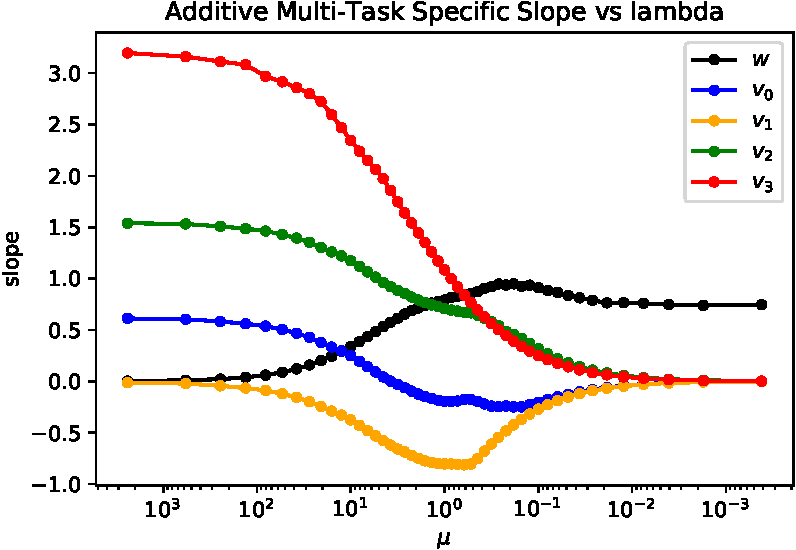
\includegraphics[width=\textwidth]{Chapter6/HAIS2019/synthetic_specWeights_add-crop.pdf}
            \end{column}
            \begin{column}{0.5\textwidth}  %%<--- here
                \begin{center}
                  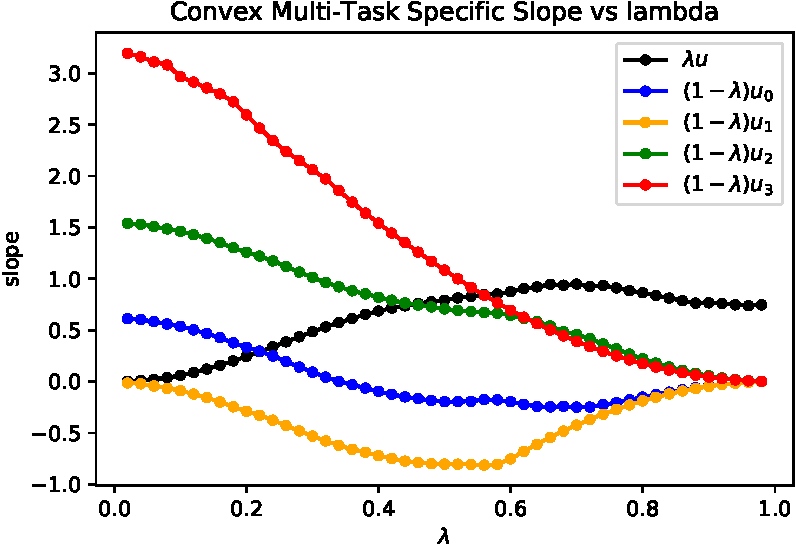
\includegraphics[width=\textwidth]{Chapter6/HAIS2019/synthetic_specWeights_conv-crop.pdf}
                 \end{center}
            \end{column}
      \end{columns}

      % 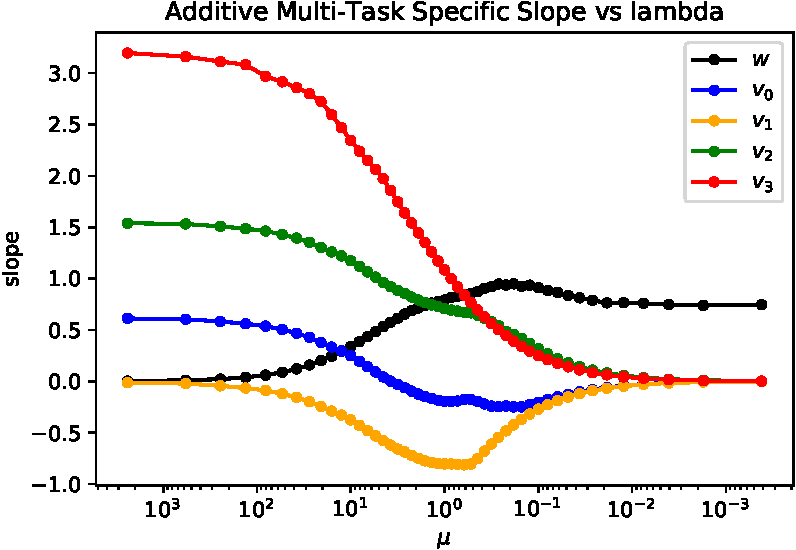
\includegraphics[width=0.45\textwidth]{Chapter6/HAIS2019/synthetic_specWeights_add-crop.pdf}

      % \begin{figure}[t!]
      %       \centering
      %       \subfloat[][{Additive} MTL slope estimates weights as a function of $\mu$. We represent the common part of the models as $w$, and the task-specific parts as $v_r$.]{%    
      %       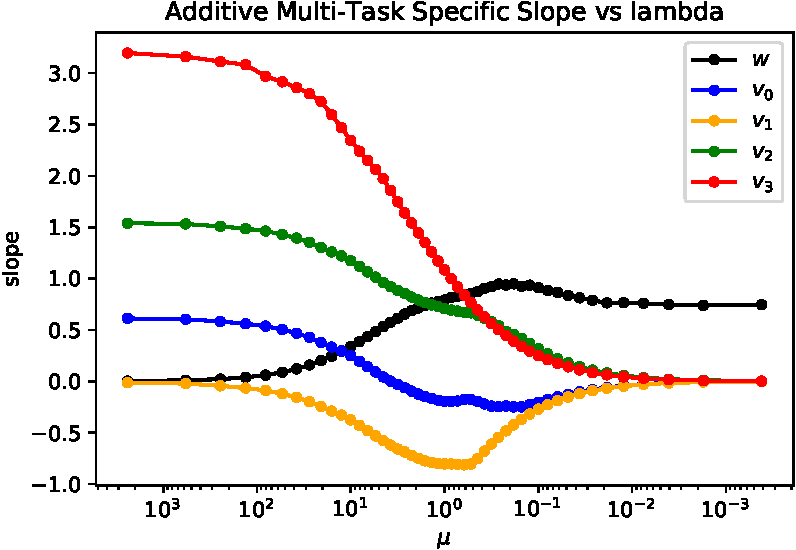
\includegraphics[width=0.45\textwidth]{Chapter6/HAIS2019/synthetic_specWeights_add-crop.pdf}
      %       \label{fig:additive_weights}}\quad%
      %       \subfloat[][{Convex} MTL slope estimates weights as a function of $\lambda$. We represent the common part of the models as $\lambda u$, and the task-specific parts as $(1 - \lambda) u_r$.]{%
      %       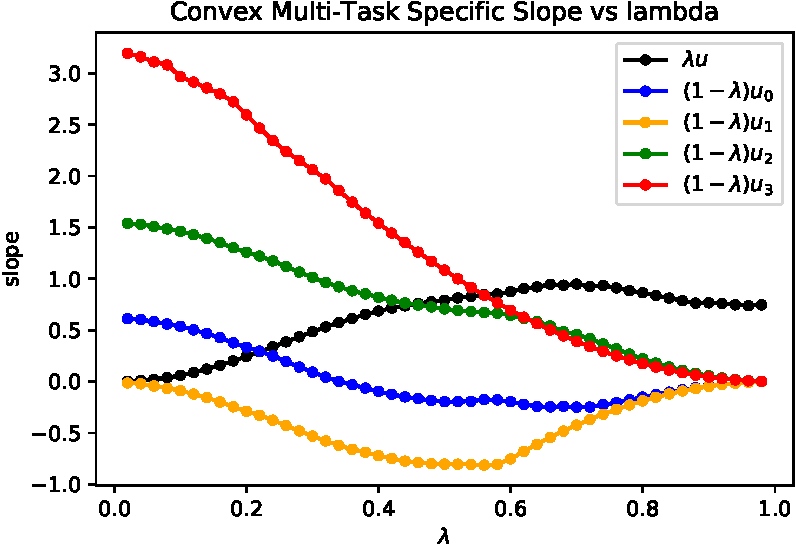
\includegraphics[width=0.45\textwidth]{Chapter6/HAIS2019/synthetic_specWeights_conv-crop.pdf}
      %       \label{fig:convex_weights}}\\
      %       \caption{Additive and Convex \acrshort{mtl}\acrshort{svr} slope estimates.}
      %       \label{fig:synthetic_specWeights}
      %   \end{figure}

\end{frame}



\begin{frame}
      \frametitle{Formulación Convexa para L2-SVM MT}

      \begin{block}{Problema Primal - MTL L2-SVM Convexa}
            \begin{equation}\nonumber
                  \begin{aligned}
                  & \argmin_{w, \fv{v}, b, \fv{d}, \xi}
                  & & {J({w}, \fv{v}, b, \fv{d}, \fv{\xi}) = \frac{C}{2} \sum_{r= 1}^T \sum_{i=1}^{m_r} ({\xi_{i}^r})^2 + \frac{1}{2} \sum_{r= 1}^T{\norm{{v}_r}^2} + \frac{1}{2} {\norm{{w}}}^2} \\
                  & \text{s.t.}
                  & & y_{i}^r \left(\lambda_r \left\lbrace \dotp{w}{\phi(x_{i}^r)} + b  \right\rbrace + (1 - \lambda_r) \left\lbrace \dotp{{v}_r}{\phi_r(x_{i}^r)} + d_r \right\rbrace  \right) \geq p_{i}^r - \xi_{i}^r ,  \\
                  \end{aligned}
              \end{equation}
      \end{block}

      \begin{block}{Problema Dual - MTL L2-SVM Convexa}
            \begin{equation}\nonumber
                  \begin{aligned}
                  & \min_{\alpha} && \Theta(\alpha) = \frac{1}{2} \fv{\alpha}^\intercal \left( \left\lbrace \Lambda \fm{Q} \Lambda + \left(\fm{I}_{\nsamples} - \Lambda \right) \fm{K} \left(\fm{I}_{\nsamples} - \Lambda \right) \right\rbrace + \frac{1}{C} \fm{I} \right) \fv{\alpha} - \fv{p} \fv{\alpha} \\
                  & \text{s.t.}
                  & & 0 \leq \alpha_i^r , \; i=1, \ldots, \npertask_r,\; r=1, \ldots, \ntasks, \\
                  & & & \sum_{i=1}^{m_r} \alpha_i^r y_i^r = 0, \;  r=1, \ldots, \ntasks . \\
                  \end{aligned}
              \end{equation}
      \end{block}
      

\end{frame}


% \begin{frame}
%       \frametitle{Extensiones a L2 y LS-SVM}

%       \begin{itemize}
%             \item En la SVM (L1-SVM) hemos definido los modelos:
%             \begin{equation}
%                   \nonumber
%                   h_r(\cdot) = \lambda_r \left\lbrace \dotp{w}{\phi(\cdot)} + b  \right\rbrace + (1 - \lambda_r) \left\lbrace \dotp{{v}_r}{\phi_r(\cdot)} + d_r \right\rbrace
%             \end{equation}
%       \end{itemize}

% \end{frame}


% \begin{frame}
%       \frametitle{Formulación Convexa para L2-SVM MT}
  
%       \begin{block}{Problema Dual - MTL L2-SVM Convexa}
%             \begin{equation}\nonumber
%                   \begin{aligned}
%                   & \min_{\alpha} && \Theta(\alpha) = \frac{1}{2} \fv{\alpha}^\intercal \left( \left\lbrace \Lambda \fm{Q} \Lambda + \left(\fm{I}_{\nsamples} - \Lambda \right) \fm{K} \left(\fm{I}_{\nsamples} - \Lambda \right) \right\rbrace + \frac{1}{C} \fm{I} \right) \fv{\alpha} - \fv{p} \fv{\alpha} \\
%                   & \text{s.t.}
%                   & & 0 \leq \alpha_i^r , \; i=1, \ldots, \npertask_r,\; r=1, \ldots, \ntasks, \\
%                   & & & \sum_{i=1}^{m_r} \alpha_i^r y_i^r = 0, \;  r=1, \ldots, \ntasks . \\
%                   \end{aligned}
%               \end{equation}
%       \end{block}

%   \end{frame}


  \begin{frame}
      \frametitle{Formulación Convexa para LS-SVM MT}

      \begin{block}{Problema Primal - MTL LS-SVM Convexa}
            \begin{equation}\nonumber
                  \begin{aligned}
                  & \argmin_{w, \fv{v}, b, \fv{d}, \xi}
                  & & {J({w}, \fv{v}, b, \fv{d}, \fv{\xi}) = \frac{C}{2} \sum_{r= 1}^T \sum_{i=1}^{m_r} \left({\xi_{i}^r}\right)^2 + \frac{1}{2} \sum_{r= 1}^T{\norm{{v}_r}^2} + \frac{1}{2} {\norm{{w}}}^2} \\
                  & \text{s.t.}
                  & & y_{i}^r \left(\lambda_r \left\lbrace \dotp{w}{\phi(x_{i}^r)} + b  \right\rbrace + (1 - \lambda_r) \left\lbrace \dotp{{v}_r}{\phi_r(x_{i}^r)} + d_r \right\rbrace  \right) = p_{i}^r - \xi_{i}^r ,  \\
                  \end{aligned}
              \end{equation}
      \end{block}

      \begin{block}{Problema Dual - MTL LS-SVM Convexa}
            \begin{equation}
                  \nonumber
                  \begin{aligned}
                  \left[
                  \begin{array}{c|c|c}
                  0 & \fv{0}_\ntasks^\intercal &  \fv{y}^\intercal \Lambda \\
                  \hline
                  \fv{0}_\ntasks & \fv{0}_{\ntasks \times \ntasks} & \fm{A}^\intercal \fm{y} (I_\nsamples - \Lambda)\\
                  \hline
                  \fv{y} & \fm{y} \fm{A} & \widehat{\fm{Q}} + \frac{1}{C} \fm{I}_\nsamples
                  \end{array}
                  \right] 
                  \begin{pmatrix}
                      b \\
                      d_1 \\
                      \vdots \\
                      d_\ntasks \\
                      \fv{\alpha}
                  \end{pmatrix}
                  = 
                  \begin{pmatrix}
                      0 \\
                      \fv{0}_\ntasks \\
                      \fv{p}
                  \end{pmatrix}, 
                  \end{aligned}
              \end{equation}
      \end{block}

\end{frame}










% \begin{frame}
%       \frametitle{Formulación Convexa para LS-SVM MT}
  
%       \begin{block}{Problema Dual - MTL LS-SVM Convexa}
%             \begin{equation}
%                   \nonumber
%                   \begin{aligned}
%                   \left[
%                   \begin{array}{c|c|c}
%                   0 & \fv{0}_\ntasks^\intercal &  \fv{y}^\intercal \Lambda \\
%                   \hline
%                   \fv{0}_\ntasks & \fv{0}_{\ntasks \times \ntasks} & \fm{A}^\intercal \fm{y} (I_\nsamples - \Lambda)\\
%                   \hline
%                   \fv{y} & \fm{y} \fm{A} & \widehat{\fm{Q}} + \frac{1}{C} \fm{I}_\nsamples
%                   \end{array}
%                   \right] 
%                   \begin{pmatrix}
%                       b \\
%                       d_1 \\
%                       \vdots \\
%                       d_\ntasks \\
%                       \fv{\alpha}
%                   \end{pmatrix}
%                   = 
%                   \begin{pmatrix}
%                       0 \\
%                       \fv{0}_\ntasks \\
%                       \fv{p}
%                   \end{pmatrix}, 
%                   \end{aligned}
%               \end{equation}
%       \end{block}

%   \end{frame}



  


\subsection{Combinación Convexa de modelos Preentrenados}

\begin{frame}
      \frametitle{Combinación Convexa de modelos Preentrenados}

      \begin{itemize}
            \item Alternativa a la formulación convexa para aprendizaje MT
            \item Consideramos la combinación convexa de
            \begin{itemize}
                  \item modelo común $g(\cdot)$ entrenado
                  \item modelos específicos $g_r(\cdot)$ entrenados
            \end{itemize}
            \item Minimizamos el riesgo eligiendo los hiperparámetros $\lambda_1, \ldots, \lambda_\ntasks$ óptimos
            \begin{equation}
                  \nonumber
                  \emprisk(\lambda_1, \ldots, \lambda_\ntasks) = \sum_{r=1}^\ntasks \sum_{i=1}^{\npertask_r} \lossf(\lambda_r g(x_i^r) + (1 - \lambda_r) g_r(x_i^r), y_i^r) ,
              \end{equation}

      \end{itemize}

\end{frame}



\begin{frame}
      \frametitle{Formulación Unificada Clasificación}

      \begin{itemize}
            \item Hinge loss (classification):
            \begin{equation}
                \nonumber%\label{eq:hingeloss_emprisk}
                \emprisk(\lambda_1, \ldots, \lambda_\ntasks) = \sum_{r=1}^\ntasks \sum_{i=1}^{\npertask_r} \pospart{1 - y_i^r \left\lbrace\lambda_r g(x_i^r) + (1 - \lambda_r) g_r(x_i^r) \right \rbrace} .
            \end{equation}
            \item Squared hinge loss (classification):
            \begin{equation}
                \nonumber%\label{eq:sqhingeloss_emprisk}
                \emprisk(\lambda_1, \ldots, \lambda_\ntasks) = \sum_{r=1}^\ntasks \sum_{i=1}^{\npertask_r} \pospart{1 - y_i^r \left\lbrace\lambda_r g(x_i^r) + (1 - \lambda_r) g_r(x_i^r) \right \rbrace}^2 .
            \end{equation}
            \item Ambas se pueden expresar como:
            \begin{equation}
                  \nonumber
                  \sum_{r=1}^\ntasks \sum_{i=1}^{\npertask_r} u(\lambda_r c_i^r + d_i^r) , \; \text{donde} \; c_i^r =  y_i^r (g_r(x_i^r) - g(x_i^r))  , \;  d_i^r =  1 - y_i^r g_r(x_i^r)
              \end{equation}
            %   donde
            %   \begin{equation}
            %       \label{eq:changevar_clas}
            %       c_i^r =  y_i^r (g_r(x_i^r) - g(x_i^r))  , \;  d_i^r =  1 - y_i^r g_r(x_i^r) ,
            %   \end{equation}
        \end{itemize}

\end{frame}


\begin{frame}
      \frametitle{Formulación Unificada Regresión}

      \begin{itemize}
            \item Absolute loss (regression):
            \begin{equation}
                \nonumber%\label{eq:absloss_emprisk}
                \emprisk(\lambda_1, \ldots, \lambda_\ntasks) = \sum_{r=1}^\ntasks \sum_{i=1}^{\npertask_r} \abs{y_i^r - \left\lbrace\lambda_r g(x_i^r) + (1 - \lambda_r) g_r(x_i^r) \right \rbrace} .
            \end{equation}
            \item Squared loss (regression):
            \begin{equation}
                \nonumber%\label{eq:sqloss_emprisk}
                \emprisk(\lambda_1, \ldots, \lambda_\ntasks) = \sum_{r=1}^\ntasks \sum_{i=1}^{\npertask_r} \left( {y_i^r - \left\lbrace\lambda_r g(x_i^r) + (1 - \lambda_r) g_r(x_i^r) \right \rbrace} \right)^2 .
            \end{equation}
            \item Ambas se pueden expresar como:
            \begin{equation}
                  \nonumber
                  \sum_{r=1}^\ntasks \sum_{i=1}^{\npertask_r} u(\lambda_r c_i^r + d_i^r) ,\; \text{donde} \; c_i^r = g(x_i^r) - g_r(x_i^r)  , \;  d_i^r =  g_r(x_i^r) - y_i^r
              \end{equation}
            % donde $c_i^r = g(x_i^r) - g_r(x_i^r)  , \;  d_i^r =  g_r(x_i^r) - y_i^r .$
            %   \begin{equation}
            %       \label{eq:changevar_reg}
            %       c_i^r = g(x_i^r) - g_r(x_i^r)  , \;  d_i^r =  g_r(x_i^r) - y_i^r .
            %   \end{equation}
        \end{itemize}

\end{frame}

\begin{frame}
      \frametitle{Formulación Unificada}

      \begin{itemize}
            \item En todos los casos tenemos que minimizar 
            \begin{equation}
                  \nonumber
                  \emprisk(\lambda_1, \ldots, \lambda_\ntasks) =
                  \sum_{r=1}^\ntasks \sum_{i=1}^{\npertask_r} u(\lambda_r c_i^r + d_i^r)
            \end{equation}
            \item Como es separable, tenemos en cada tarea el problema
            \begin{equation}
                  \nonumber
                  \argmin_{\lambda_r \in [0, 1]} \mathcal{J}(\lambda_r) = \sum_{i=1}^{\npertask_r} u(\lambda_r c_i^r + d_i^r),
            \end{equation}
            \item Usando el Teorema de Fermat
            \begin{equation}
                  \nonumber
                  \lambda^* = \argmin_{0 \leq \lambda \leq 1} \mathcal{J}(\lambda) \iff (0 \in \partial \mathcal{J}(\lambda^*) \text{ and } \lambda^* \in (0, 1) ) \text{ or } \lambda^*=0 \text{ or } \lambda^*=1 .
              \end{equation}
      \end{itemize}

\end{frame}


\begin{frame}
      \frametitle{Combinación Convexa con Error Cuadrático}

      \begin{itemize}
            \item La función a minimizar es 
            \begin{equation}
                  \nonumber
                  %\label{eq:opt_sq}
                  \argmin_{\lambda \in [0, 1]} \mathcal{J}(\lambda) = \sum_{i=1}^{\npertask} \left({\lambda c_i + d_i}\right)^2 .
            \end{equation}
            \item La derivada es
            \begin{equation}
                  \nonumber
                  \mathcal{J}'(\lambda) = \sum_{i=1}^\npertask 2 c_i (\lambda c_i + d_i) .
            \end{equation}
            \item Como es derivable, resolviendo $\mathcal{J}'(\lambda)= 0$ obtenemos
            \begin{equation*}
                  \lambda' =  -\frac{\sum_{i=1}^{\npertask} d_i c_i }{\sum_{i=1}^{\npertask} (c_i)^2 } .
                  \end{equation*}
            \item La solución es entonces $\opt{\lambda} = \max(\min(\lambda', 1), 0)$
      \end{itemize}
        %
        
\end{frame}


\begin{frame}

      \begin{figure}[t!]
            \centering
            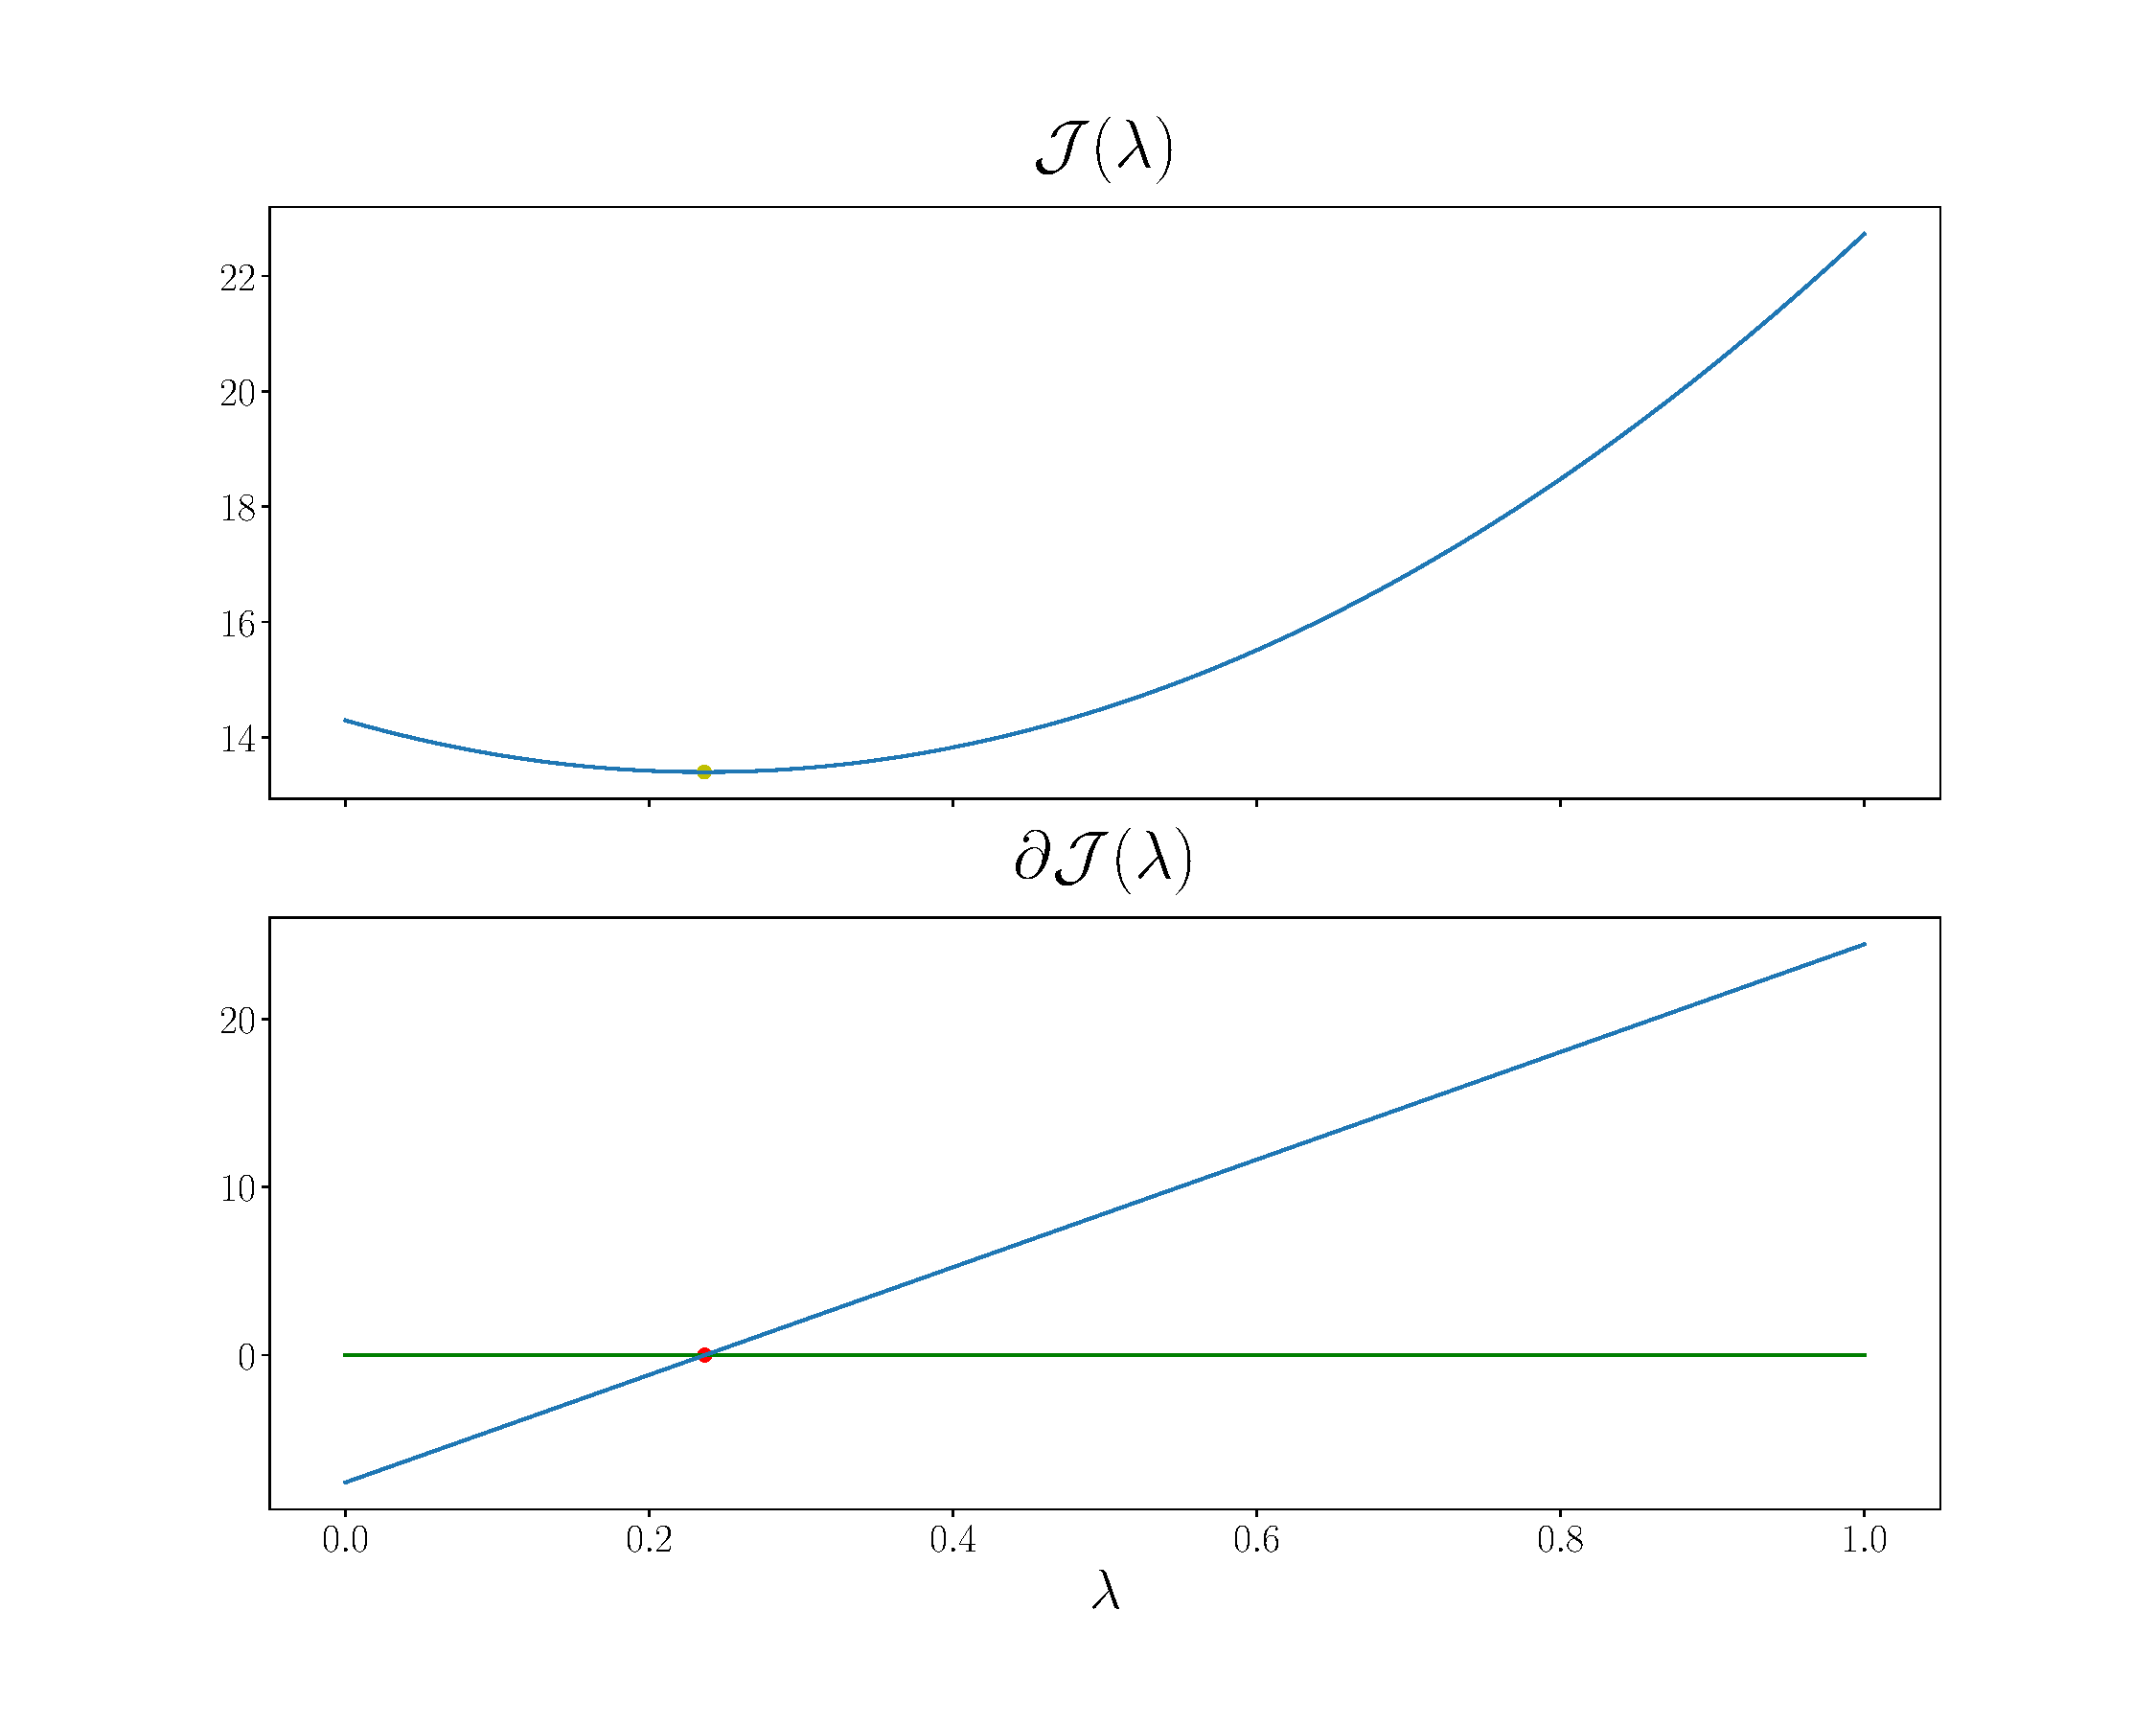
\includegraphics[width=.6\textwidth]{Chapter4/NeuroCom2021/ejemplo2_mse.pdf}
            \caption{Error using the squared loss function (top) and its corresponding derivative (bottom). The green line represents the $0$ constant function. The yellow dot is the point minimizing the error, and whose corresponding derivative contains the value $0$.}
            \label{fig:sq_error}
        \end{figure}      

\end{frame}



\begin{frame}
      \frametitle{Combinación Convexa con Error Absoluto}

      \begin{proposition}[$\lambda^*$ óptimo para el problema con valor absoluto]\label{prop:abs_neurocom2020}
            \begin{itemize}
                  \item $\lambda^*=0$ es óptimo si y solo si: $- \sum_{i: \; 0 > \lambda_{(i)}} \abs{c_{(i)}} + \sum_{i: \; 0 < \lambda_{(i)}} \abs{c_{(i)}} \leq 0$
                  \item $\lambda^* \in (0,1)$ es óptimo si y solo si $0 < \lambda^* = \lambda_{(k)} < 1$ para algún $k=1, \dotsc, \npertask$, y
                  \begin{equation}
                  \nonumber    
                  - \sum_{i:\; \lambda_{(k)} > \lambda_{(i)}} \abs{c_{(i)}} + \sum_{i:\; \lambda_{(k)} < \lambda_{(i)}} \abs{c_{(i)}} \in \left[ -  \abs{c_{(k)}},  \abs{c_{(k)}}  \right] 
                  \end{equation}
                  \item $\lambda^*=1$ es óptimo en otro caso
            \end{itemize}
        \end{proposition}
\end{frame}


\begin{frame}

      \begin{figure}[t!]
            \centering
            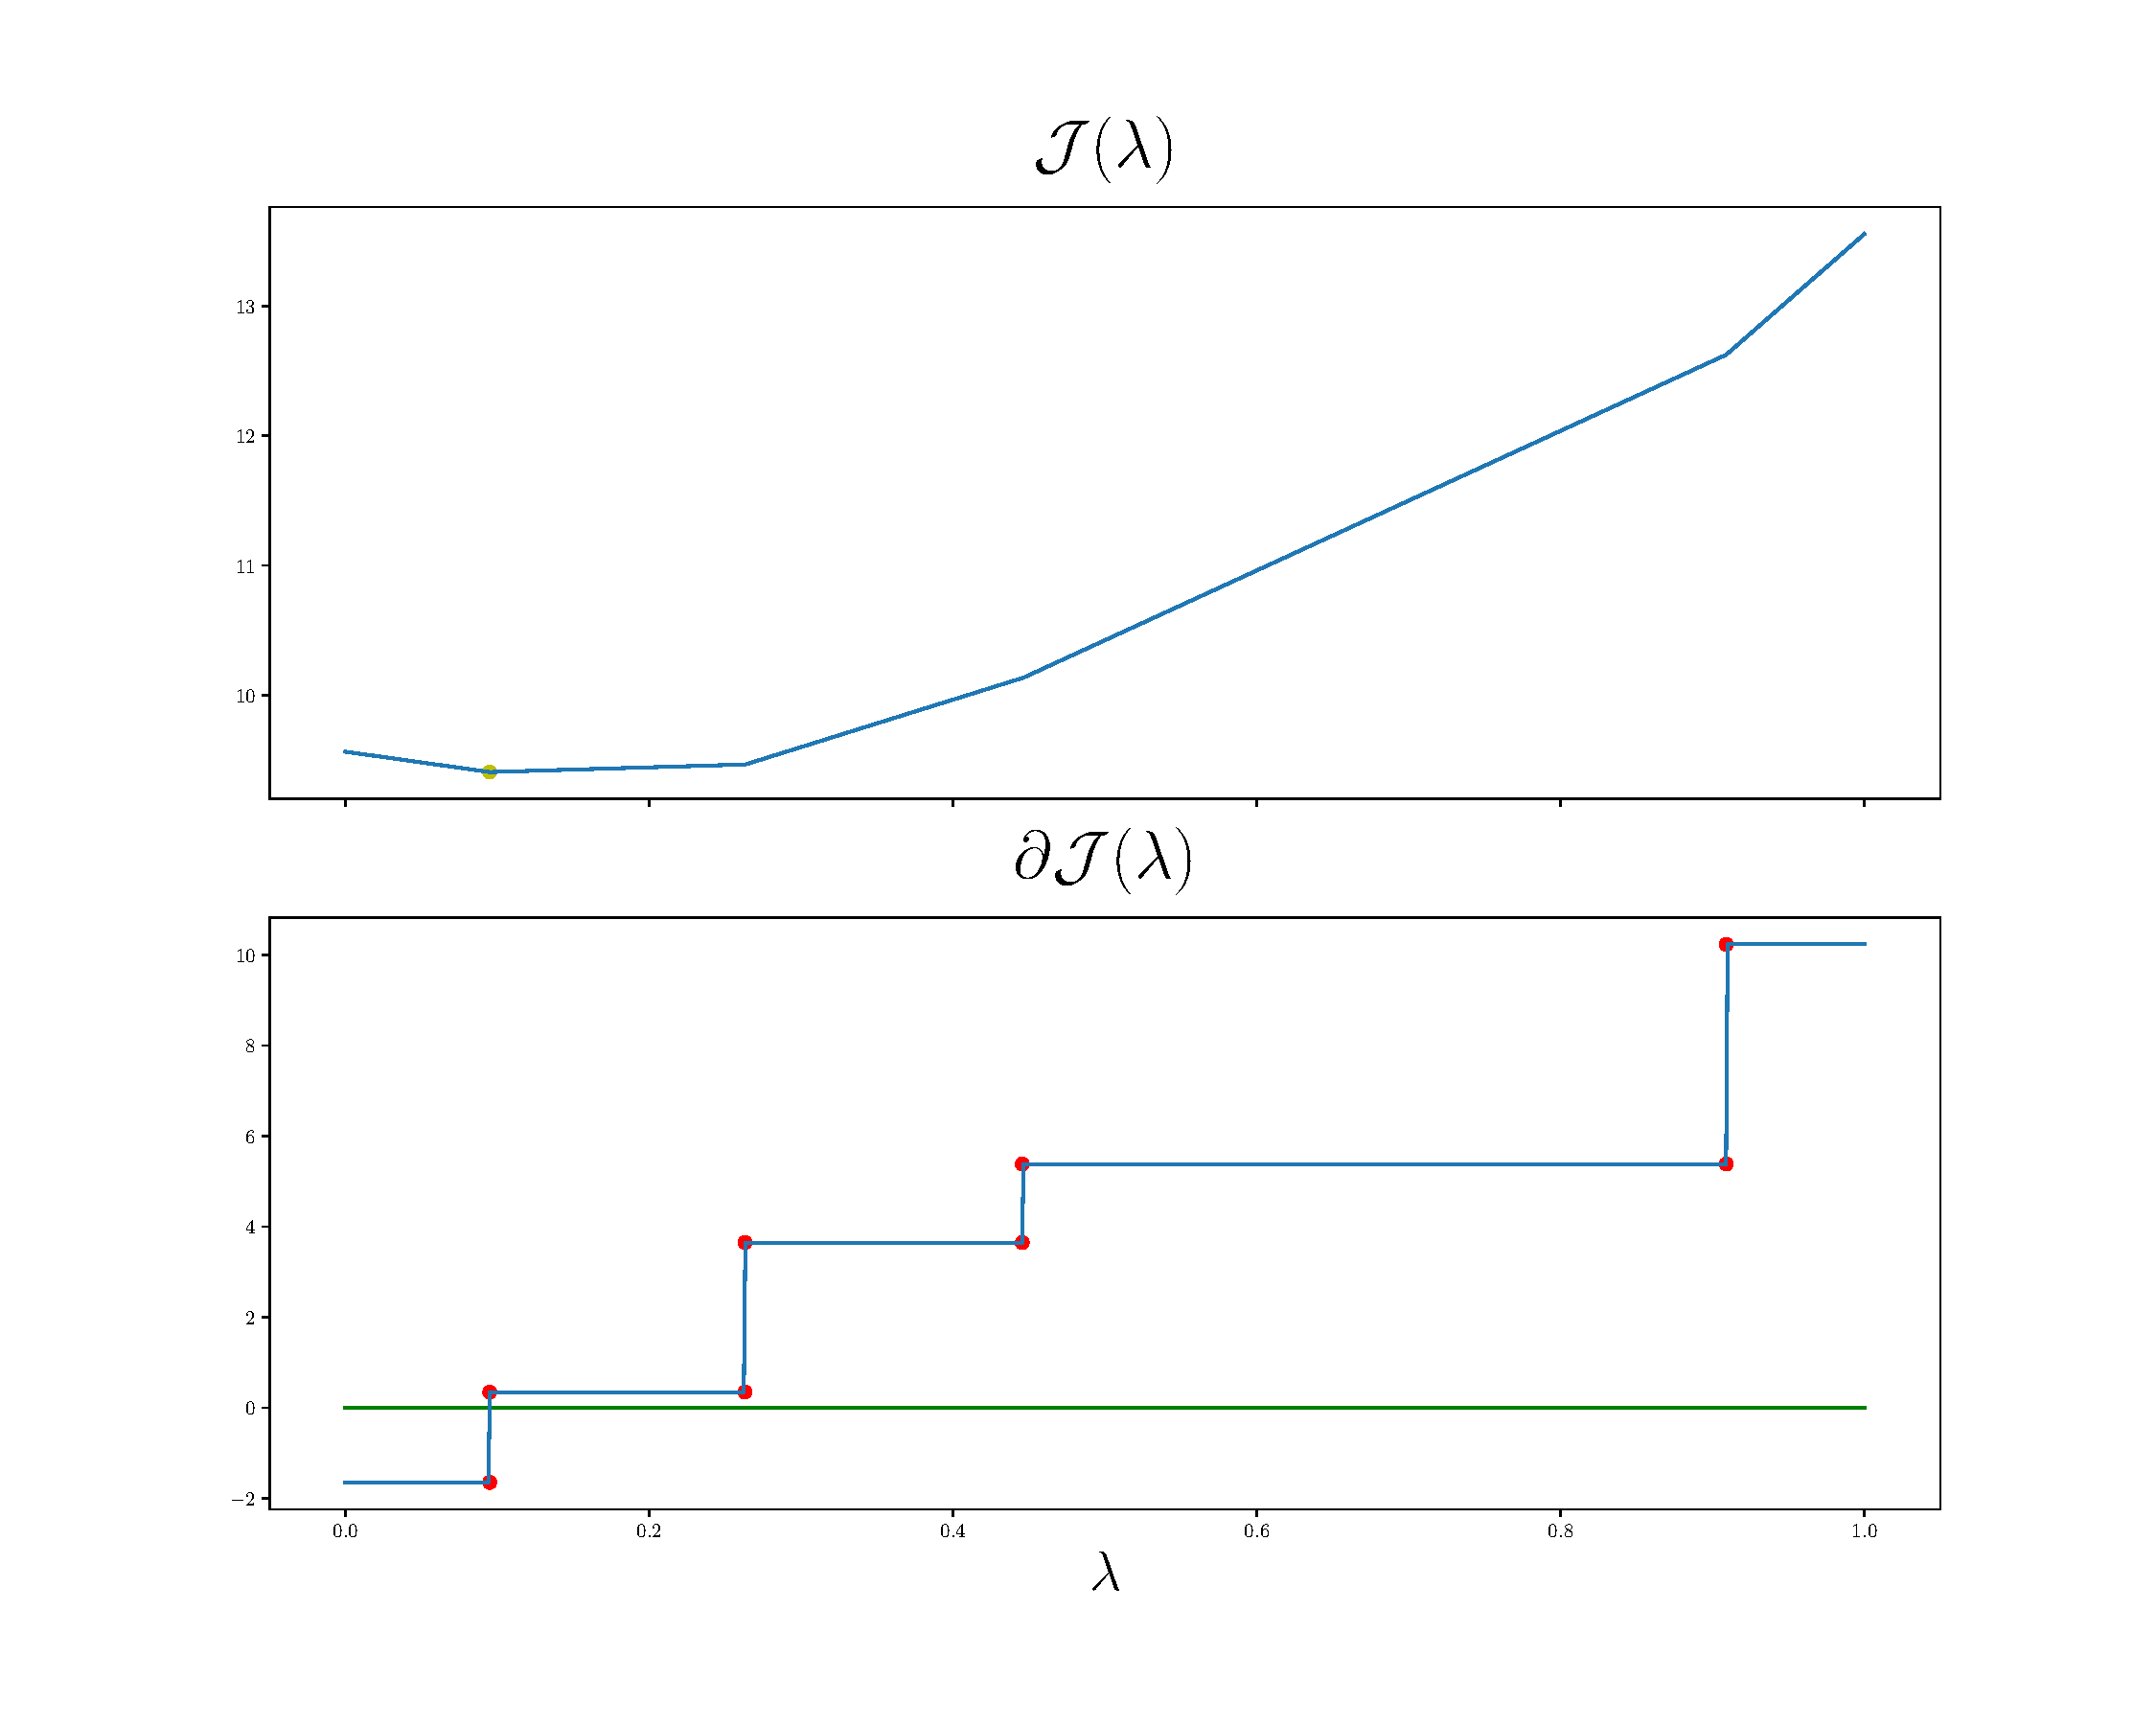
\includegraphics[width=.6\textwidth]{Chapter4/NeuroCom2021/ejemplo2_mae.pdf}
            \label{fig:sq_error}
        \end{figure}      

\end{frame}




\begin{frame}
      \frametitle{Combinación Convexa con Error Hinge}
      \begin{proposition}[$\lambda^*$ óptimo para el problema con error hinge]\label{prop:hinge_neurocom2020}
            \begin{itemize}
                  \item $\lambda^*=0$ es óptimo si y solo si: $-\sum_{i:\; 0 > \lambda_{(i)}} \mymax{0, c_{(i)}} - \sum_{0 < \lambda_{(i)}} \mymin{0, c_{(i)}} \leq 0 $
                  \item $\lambda^* \in (0,1)$ es óptimo si y solo si $0 < \lambda^* = \lambda_{(k)} < 1$ para algún $k=1, \dotsc, \npertask$, y
                  \begin{equation}
                        \nonumber%\label{eq:sol_hinge}
                        -\sum_{i:\; \lambda_{(k)} > \lambda_{(i)}} \mymax{0, c_{(i)}} - \sum_{i:\; \lambda_{(k)} <\lambda_{(i)}} \mymin{0, c_{(i)}} \in \left[\mymin{0, c_{(k)}}, \mymax{0, c_{(k)}} \right] 
                  \end{equation}
                  \item $\lambda^*=1$ es óptimo en otro caso
            \end{itemize}
        \end{proposition}
      % \begin{proposition}[Optimal $\lambda^*$ with Hinge Loss]\label{prop:hinge_neurocom2020}
      %       In~\eqref{eq:opt_hinge_l1}, $\lambda^*=0$ is optimal iff
      %       \begin{equation}
      %           \nonumber
      %           %\label{eq:sol_hinge_0}
      %           -\sum_{i:\; 0 > \lambda_{(i)}} \mymax{0, c_{(i)}} - \sum_{0 < \lambda_{(i)}} \mymin{0, c_{(i)}} \leq 0 .
      %           \end{equation}
      %           If this condition does not hold, a value $\lambda^* \in (0, 1)$ is optimal for problem~\eqref{eq:opt_hinge_l1} \emph{iff} $\lambda^*$ is a feasible elbow, that is, $0 < \lambda^* = \lambda_{(k)} < 1$ for some $k=1, \dotsc, \npertask$, and
      %       \begin{equation}
      %           \label{eq:sol_hinge}
      %           -\sum_{i:\; \lambda_{(k)} > \lambda_{(i)}} \mymax{0, c_{(i)}} - \sum_{i:\; \lambda_{(k)} <\lambda_{(i)}} \mymin{0, c_{(i)}} \in \left[\mymin{0, c_{(k)}}, \mymax{0, c_{(k)}} \right] .
      %       \end{equation}
      %       If none of the previous conditions hold, then $\lambda^*=1$ is optimal.
      %   \end{proposition}
\end{frame}


\begin{frame}

      \begin{figure}[t!]
            \centering
            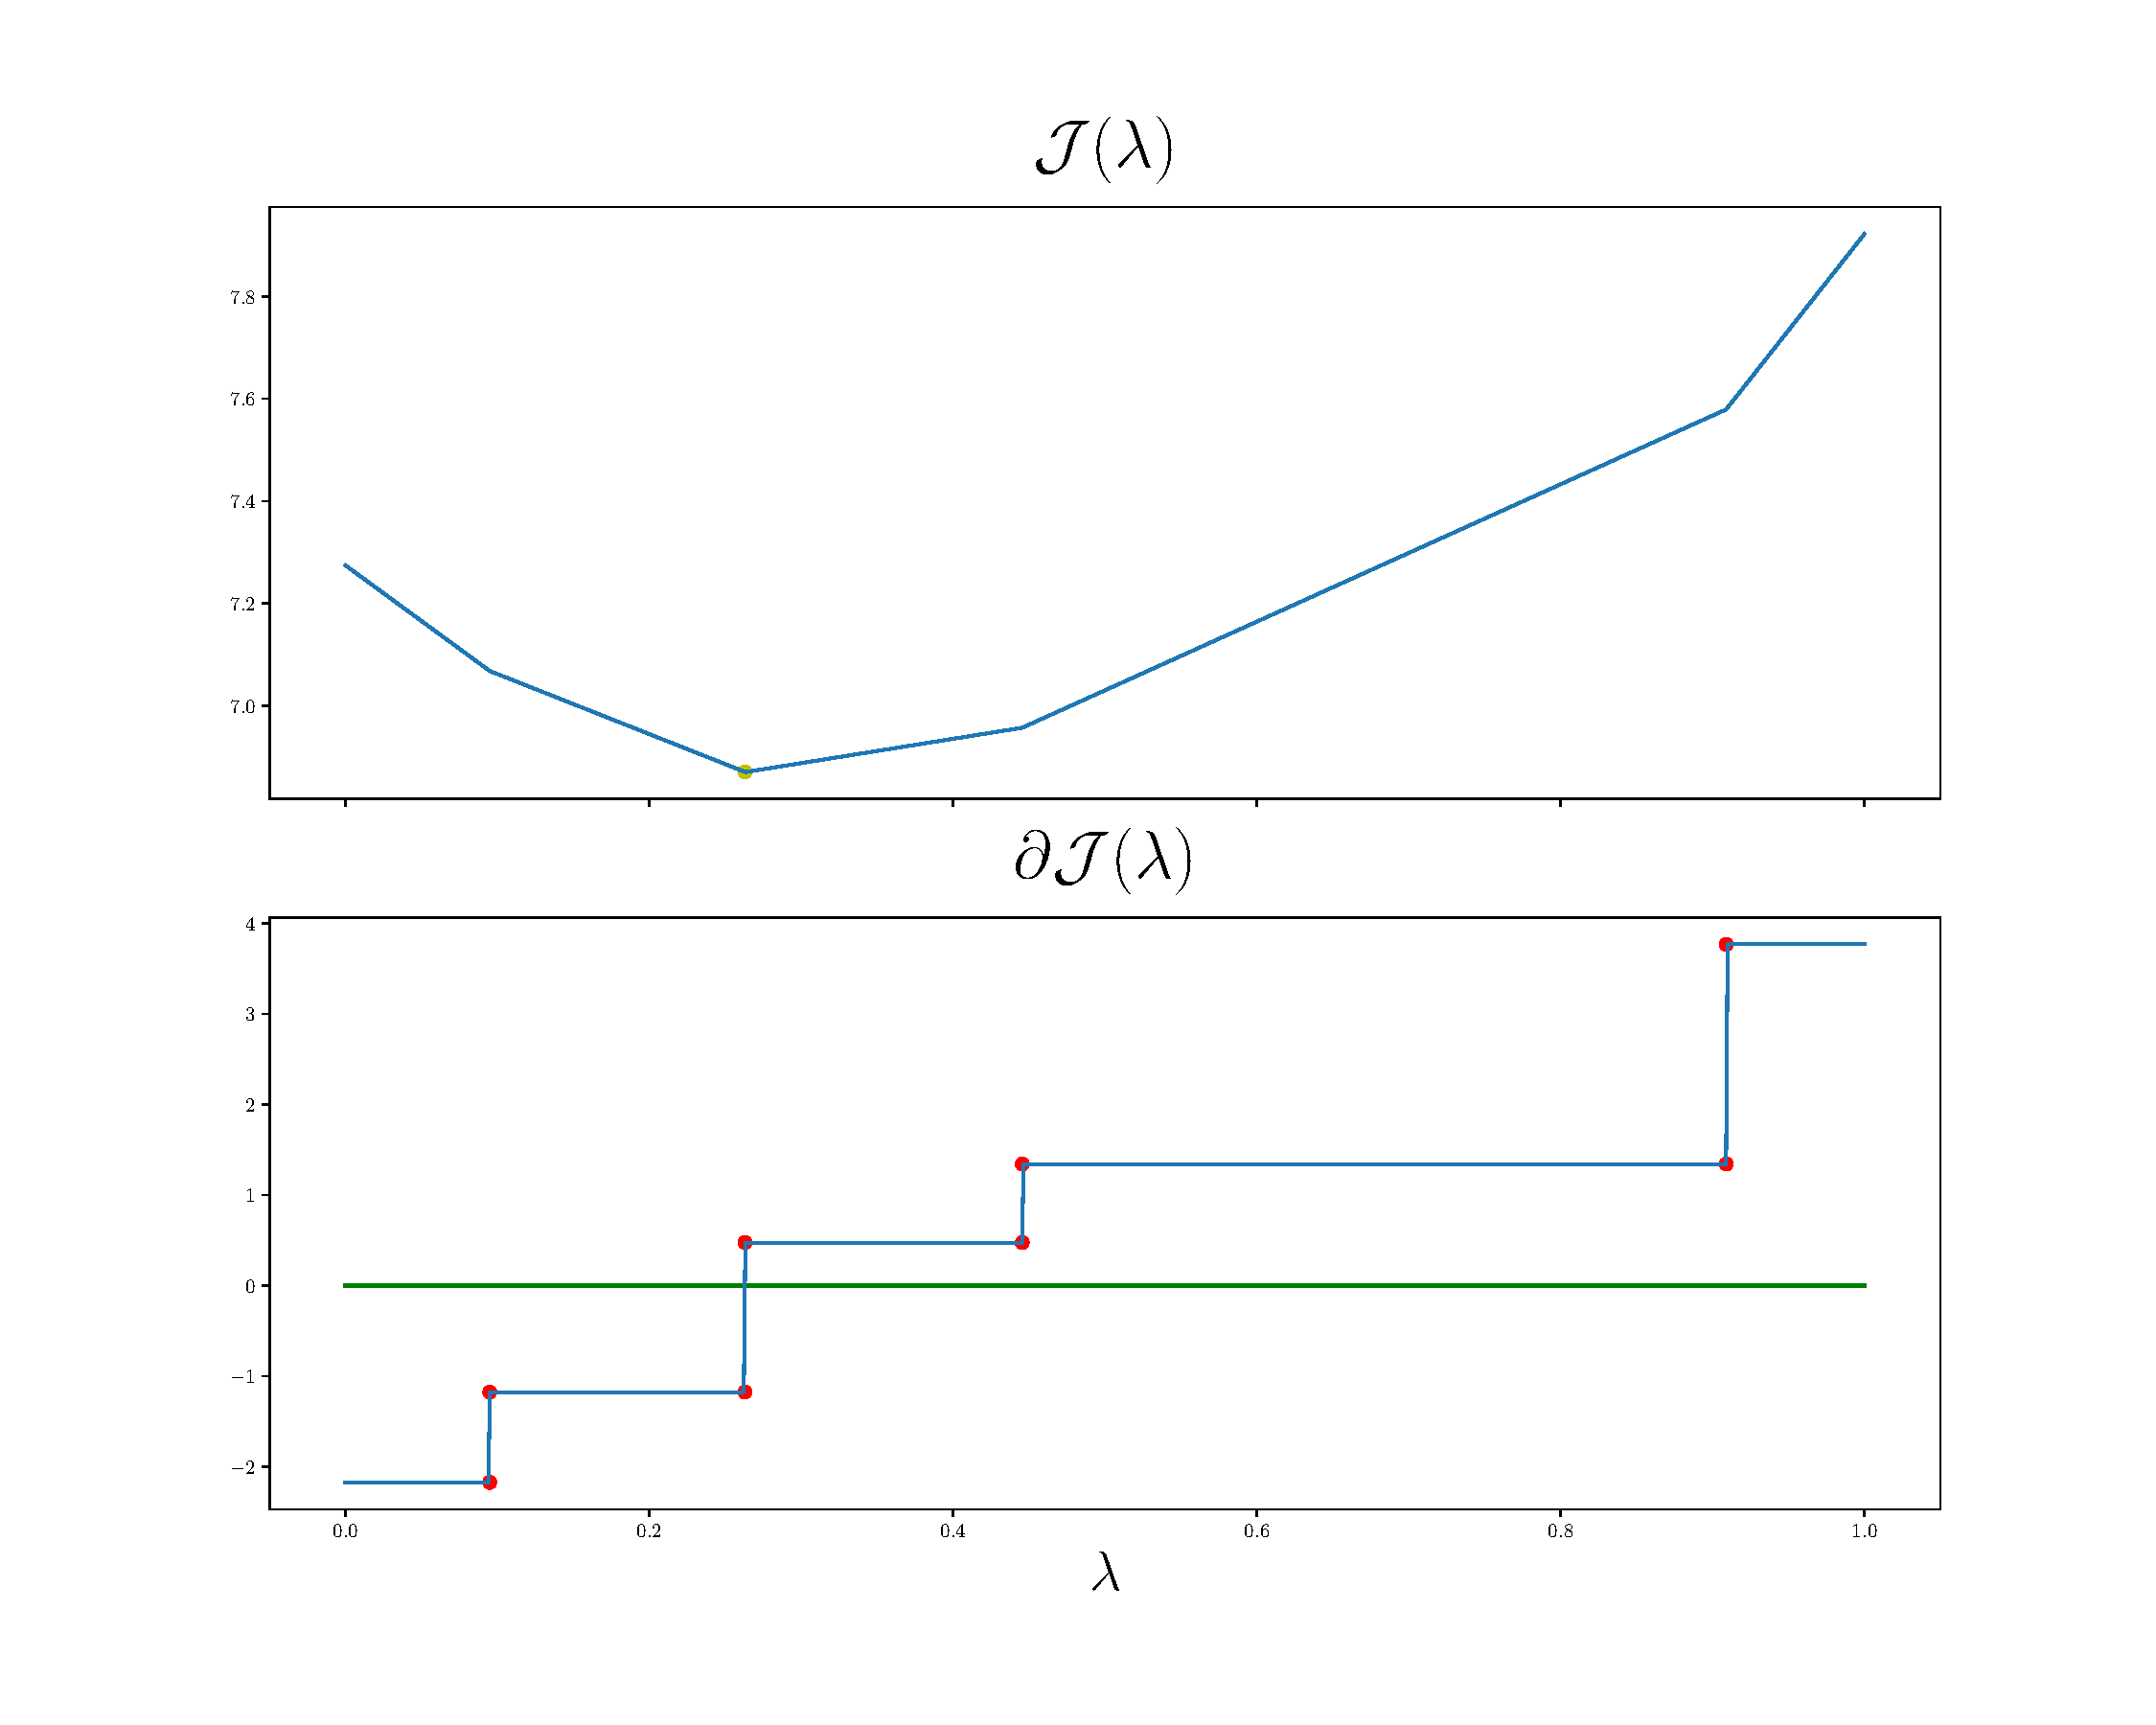
\includegraphics[width=.6\textwidth]{Chapter4/NeuroCom2021/ejemplo2_hinge.pdf}
            \label{fig:sq_error}
        \end{figure}      

\end{frame}


\begin{frame}
      \frametitle{Combinación Convexa con Error Hinge Cuadrático}


      \begin{proposition}[$\lambda^*$ óptimo para el problema con error hinge cuadrático]\nonumber%\label{prop:hinge_neurocom2020}
            \begin{itemize}
                  \item $\lambda^*=0$ es óptimo si y solo si: $-\sum_{i:\; 0 > c_{(i)}, 0 < \lambda_{(i)}} {2 c_i d_i} - \sum_{i:\; 0 < c_{(i)}, 0 > \lambda_{(i)}} {2 c_i d_i}  \leq 0 $
                  \item $\lambda^* \in (0,1)$ es óptimo si y solo si $0 < \lambda^* = \widehat{\lambda}_{(k)} < 1$ para algún $k=1, \dotsc, \npertask$, donde
                  \begin{equation}\nonumber%\label{eq:sol_hinge_2}
                        \widehat{\lambda}_{(k)} = - \frac{\sum_{i:\; \lambda_{(k+1)} \geq \lambda_{(i)}} \mymax{0, c_{(i)}} d_{(i)} + \sum_{i:\; \lambda_{(k)} \leq \lambda_{(i)}} \mymin{0, c_{(i)}} d_{(i)}}{\sum_{i:\; \lambda_{(k+1)} \geq \lambda_{(i)}} \mymax{0, c_{(i)}}^2 + \sum_{i:\; \lambda_{(k)} \leq \lambda_{(i)}} \mymin{0, c_{(i)}}^2} ,
                  \end{equation}
                  y además $\lambda_{(k)} \leq \widehat{\lambda}_k \leq  \lambda_{(k+1)}$
                  \item $\lambda^*=1$ es óptimo en otro caso
            \end{itemize}
        \end{proposition}

      % \begin{proposition}[Optimal $\lambda^*$ with Squared Hinge Loss]\label{prop:sqhinge_neurocom2020}
      %       In~\eqref{eq:opt_hinge_l2},
      %       $\lambda^*=0$ is optimal iff 
      %       \begin{equation}\nonumber
      %           -\sum_{\substack{i:\; 0 > c_{(i)},\\ \;\; 0 < \lambda_{(i)}}} {2 c_i d_i} - \sum_{\substack{i:\; 0 < c_{(i)},\\ \;\; 0 > \lambda_{(i)}}} {2 c_i d_i}  \leq 0 .
      %          \end{equation}
      %       If this condition does not hold, 
      %       consider the sorted list of elbows $\lambda_{(1)}, \ldots, \lambda_{(\npertask)}$; then, for each interval between elbows $(\lambda_{(k)}, \lambda_{(k+1)})$, we define the value $\widehat{\lambda}_k$ for $k=1, \ldots,  \npertask-1$ as %
      %   \begin{equation}\label{eq:sol_hinge_2}
      %       \widehat{\lambda}_{(k)} = - \frac{\sum_{i:\; \lambda_{(k+1)} \geq \lambda_{(i)}} \mymax{0, c_{(i)}} d_{(i)} + \sum_{i:\; \lambda_{(k)} \leq \lambda_{(i)}} \mymin{0, c_{(i)}} d_{(i)}}{\sum_{i:\; \lambda_{(k+1)} \geq \lambda_{(i)}} \mymax{0, c_{(i)}}^2 + \sum_{i:\; \lambda_{(k)} \leq \lambda_{(i)}} \mymin{0, c_{(i)}}^2} .
      %   \end{equation}
      %   %
      %   If $\widehat{\lambda}_k$ satisfies that $\lambda_{(k)} \leq \widehat{\lambda}_k \leq  \lambda_{(k+1)}$ and $0 \leq \widehat{\lambda}_{(k)} \leq 1$ for some $k=1, \ldots, \npertask$ then $\lambda^* = \widehat{\lambda}_k$ is optimal.
      %   Finally, if none of the previous conditions holds, \eqref{eq:opt_hinge_l2} has a minimum at $\lambda^* = 1$.
      %   \end{proposition}
\end{frame}

\begin{frame}

      \begin{figure}[t!]
            \centering
            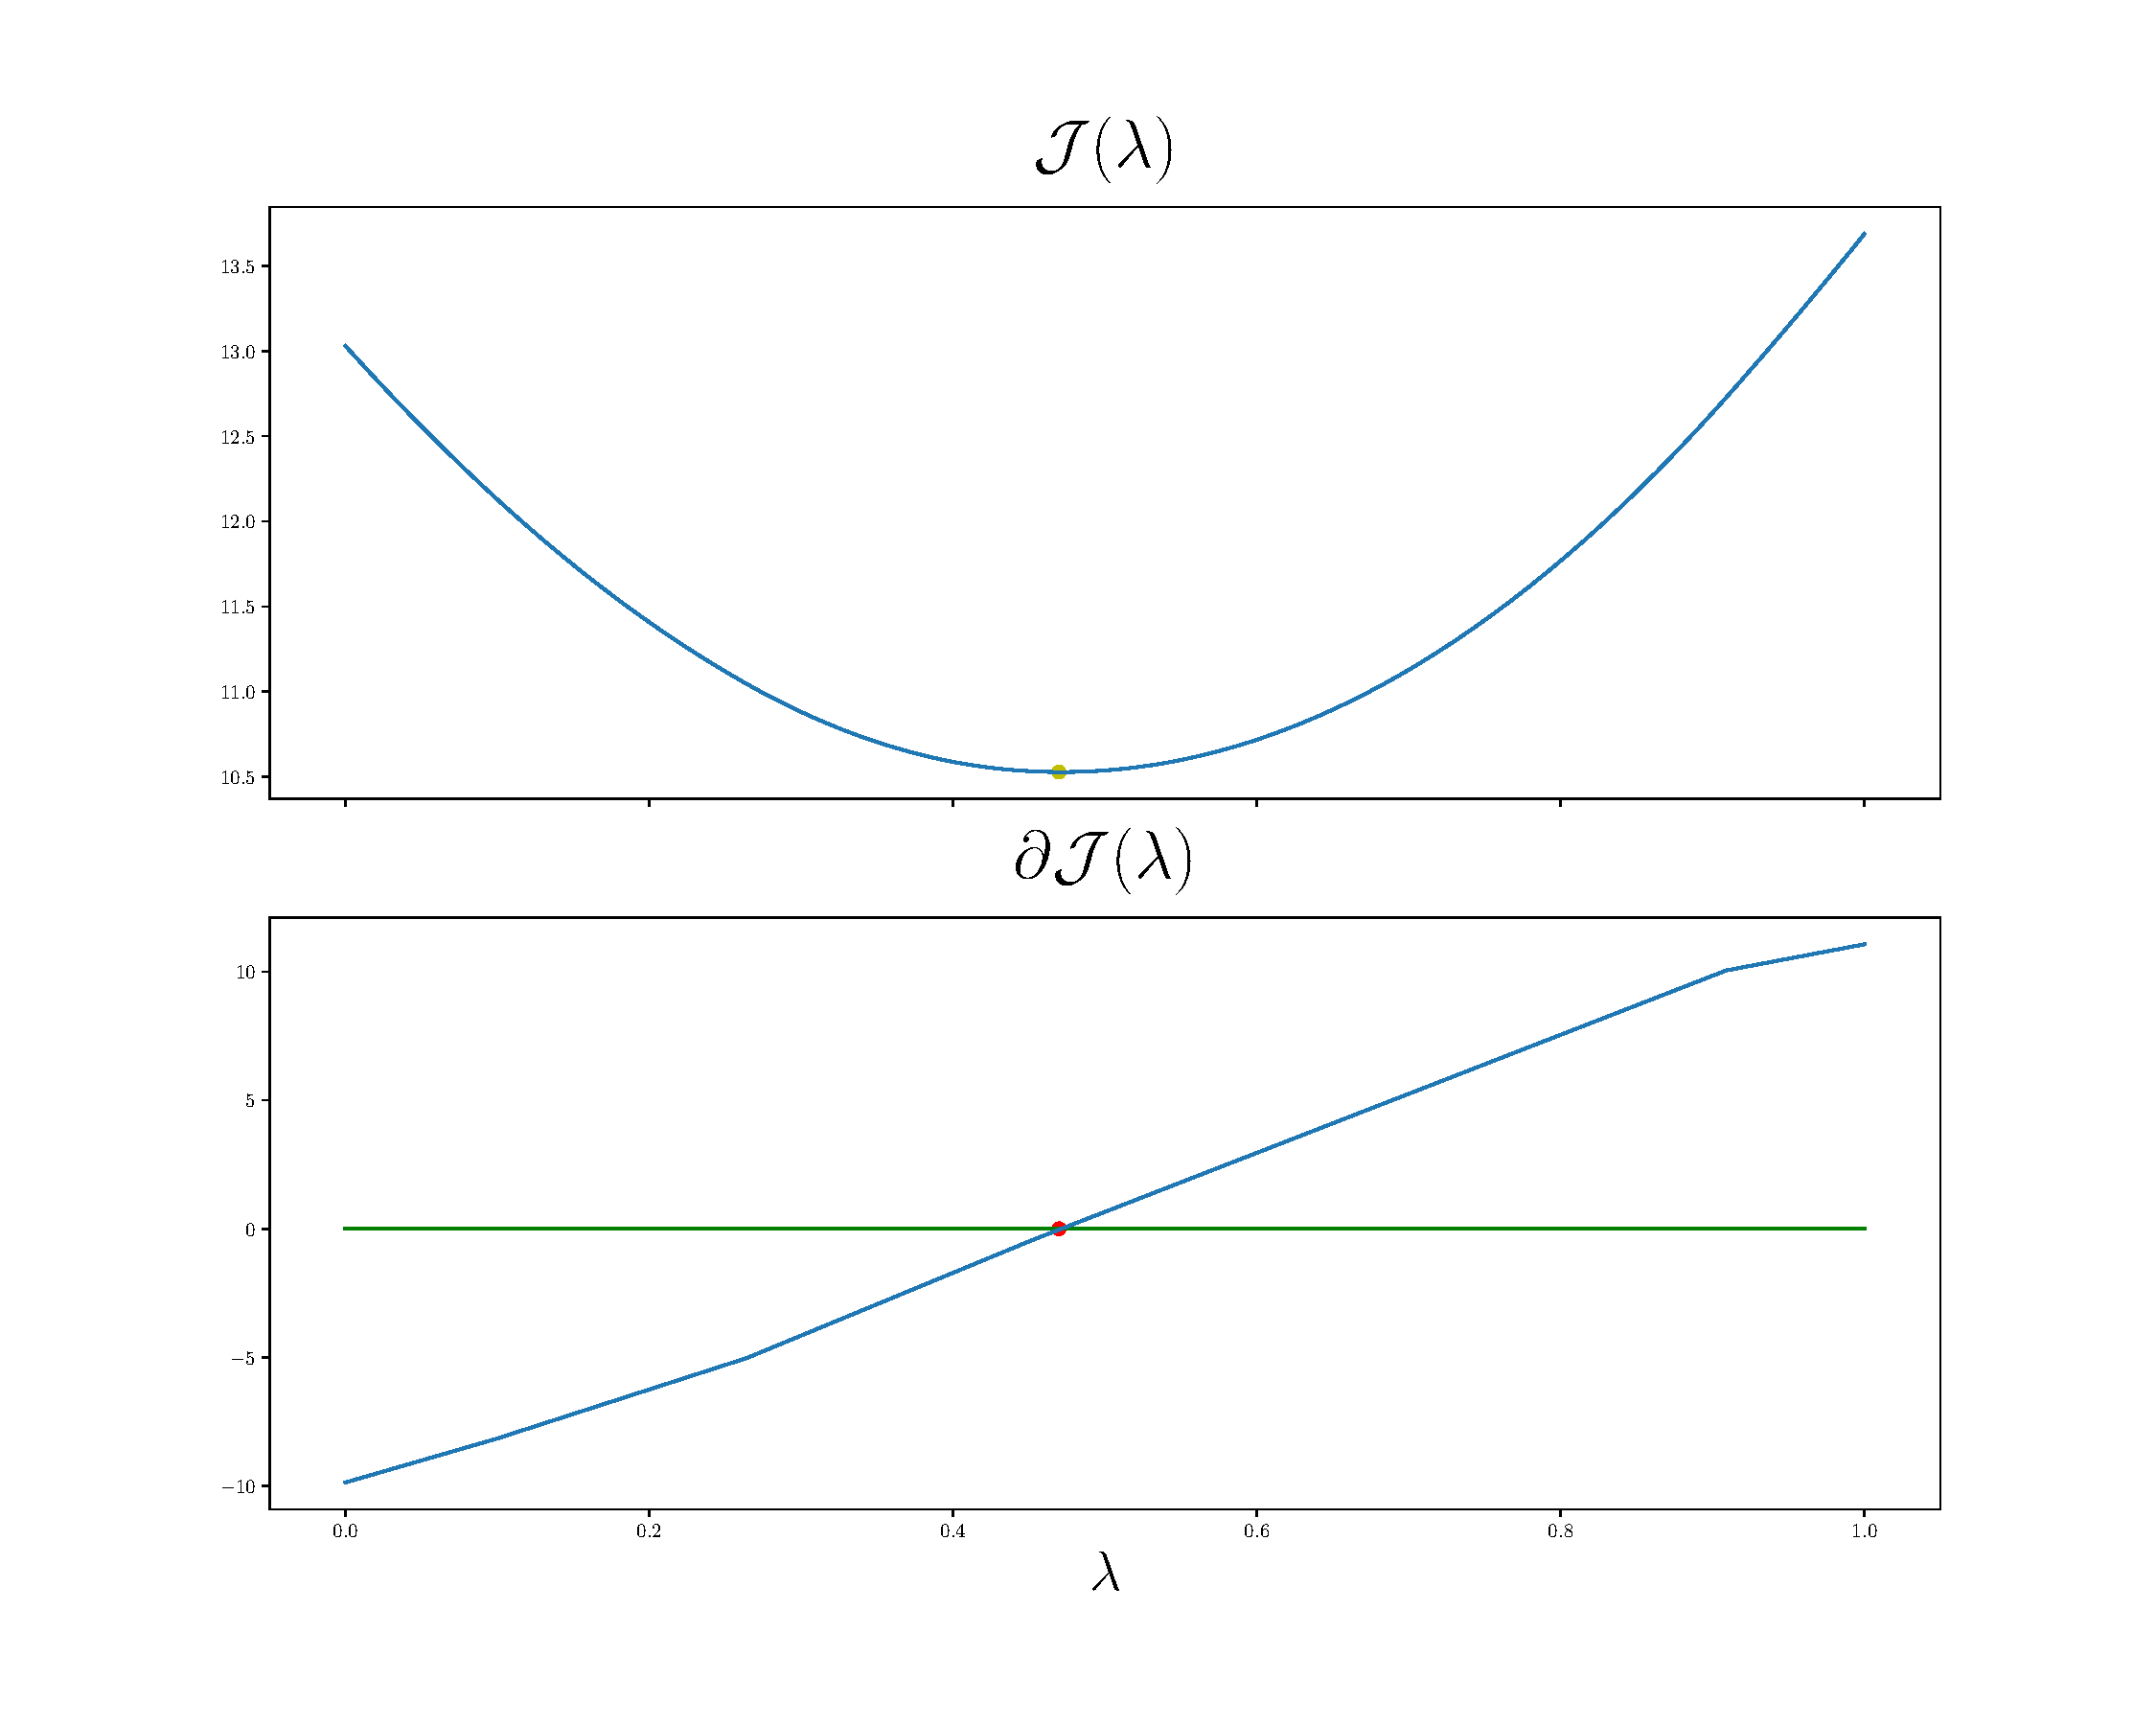
\includegraphics[width=.6\textwidth]{Chapter4/NeuroCom2021/ejemplo2_sqhinge.pdf}
            \label{fig:sq_error}
        \end{figure}      

\end{frame}


% \begin{frame}
%       \frametitle{Experimentos}

      
%       \scalebox{.7}{
%       \begin{tabular}{l*{2}{c@{ }l}*{4}{r@{$\pm$}l@{ }l } }
%       \toprule
%       & \fheadmulti{2}{\fdata{maj.}} & \fheadmulti{2}{\fdata{ten.}} & \fheadmulti{3}{\fdata{boston}} & \fheadmulti{3}{\fdata{california}} &  \fheadmulti{3}{\fdata{abalone}} & \fheadmulti{3}{\fdata{crime}}\\
%       \midrule
%       & \fheadmulti{16}{MAE} \\
%       \midrule
%       \fmod{ITL-L1}            &  {5.087} &   (6) &  {5.743} &   (3) &  {2.341} & {0.229} &   \fmaxn{(1)} &  {36883.582} & {418.435} &   (2) &  {1.481} & {0.051} &   (3) &  {0.078} & {0.001} &   (2) \\
%       \fmod{CTL-L1}            &  {5.175} &   (7) &  {5.891} &   (5) &  \fmaxn{2.192} & \fmaxn{0.244} &   \fmaxn{(1)} &  {41754.337} & {270.908} &   (6) &  {1.482} & {0.050} &   (3) &  {0.078} & {0.001} &   (2) \\
%       \fmod{CMB-L1} &  \fmaxn{5.047} &   (5) &  \fmaxn{5.340} &  \fmaxn{(1)} &  {2.239} & {0.255} &   \fmaxn{(1)} &  {36880.238} & {420.417} &   \fmaxn{(1)} &  {1.470} & {0.052} &   (2) &  {0.077} & {0.002} &   (2) \\
%       \fmod{MTL-L1}     &  {5.050} &   (5) &  {5.535} &   (2) &  {2.206} & {0.292} &   \fmaxn{(1)} &  \fmaxn{36711.383} & \fmaxn{343.333} &  \fmaxn{(1)} &  \fmaxn{1.454} & \fmaxn{0.048} &  \fmaxn{(1)} &  \fmaxn{0.074} & \fmaxn{0.002} &  \fmaxn{(1)} \\
%       \midrule
%       \fmod{ITL-L2}            &  {4.952} &   (3) &  \fmaxn{5.629} &   (3) &  {2.356} & {0.300} &   \fmaxn{(1)} &  {37374.618} & {433.511} &   (5) &  {1.498} & {0.054} &   (4) &  {0.079} & {0.002} &   (2) \\
%       \fmod{CTL-L2}            &  {5.193} &   (7) &  {6.107} &   (8) &  \fmaxn{2.083} & \fmaxn{0.136} &   \fmaxn{(1)} &  {42335.612} & {163.773} &   (8) &  {1.503} & {0.047} &   (5) &  {0.080} & {0.002} &   (2) \\
%       \fmod{CMB-L2} &  {4.869} &   (3) &  {5.963} &   (6) &  {2.089} & {0.128} &   \fmaxn{(1)} &  {37374.618} & {433.511} &   (4) &  {1.494} & {0.050} &   (4) &  {0.077} & {0.003} &   (2) \\
%       \fmod{MTL-L2}     &  \fmaxn{4.854} &   (2) &  {5.784} &   (4) &  {2.089} & {0.134} &   \fmaxn{(1)} &  \fmaxn{37202.603} & \fmaxn{419.166} &   (3) &  \fmaxn{1.482} & \fmaxn{0.049} &   (3) &  \fmaxn{0.077} & \fmaxn{0.002} &   (2) \\
%       \midrule
%       \fmod{ITL-LS}            &  {4.937} &   (3) &  {5.649} &   (3) &  {2.204} & {0.116} &   \fmaxn{(1)} &  {37348.347} & {441.240} &   (4) &  {1.496} & {0.051} &   (4) &  {0.079} & {0.002} &   (2) \\
%       \fmod{CTL-LS}            &  {5.193} &   (7) &  {6.005} &   (7) &  \fmaxn{2.072} & \fmaxn{0.143} &  \fmaxn{(1)} &  {42259.492} & {146.825} &   (7) &  {1.502} & {0.052} &   (5) &  {0.079} & {0.002} &   (2) \\
%       \fmod{CMB-LS} &  {4.977} &   (4) &  \fmaxn{5.593} &   (3) &  {2.081} & {0.146} &   \fmaxn{(1)} &  {37339.179} & {430.288} &   (4) &  {1.486} & {0.049} &   (4) &  {0.079} & {0.002} &   (2) \\
%       \fmod{MTL-LS}     &  \fmaxn{4.824} &  \fmaxn{(1)} &  {5.754} &   (4) &  {2.077} & {0.152} &   \fmaxn{(1)} &  \fmaxn{37231.043} & \fmaxn{420.992} &   (4) &  \fmaxn{1.478} & \fmaxn{0.050} &   (3) &  \fmaxn{0.076} & \fmaxn{0.002} &   (2) \\
%       % \midrule
%       % & \fheadmulti{16}{R2} \\
%       % \midrule
%       % \fmod{ITL-L1}            &  {0.845} &   (6) &  {0.901} &   (7) &  {0.821} & {0.041} &   (2) &  {0.699} & {0.009} &   (7) &  {0.543} & {0.022} &   (8) &  {0.732} & {0.021} &   (3) \\
%       % \fmod{CTL-L1}            &  {0.837} &   (9) &  {0.901} &   (6) &  {0.854} & {0.036} &   \fmaxn{(1)} &  {0.639} & {0.006} &  (10) &  {0.559} & {0.014} &   (6) &  {0.740} & {0.027} &   (3) \\
%       % \fmod{CMB-L1} &  {0.844} &   (6) &  {0.905} &   (4) &  {0.845} & {0.053} &   \fmaxn{(1)} &  {0.699} & {0.009} &   (6) &  {0.555} & {0.018} &   (7) &  {0.741} & {0.029} &   (3) \\
%       % \fmod{MTL-L1}     &  \fmaxn{0.846} &   (4) &  \fmaxn{0.908} &   (2) &  \fmaxn{0.858} & \fmaxn{0.057} &   \fmaxn{(1)} &  \fmaxn{0.703} & \fmaxn{0.007} &   (6) &  \fmaxn{0.568} & \fmaxn{0.012} &   (5) &  \fmaxn{0.760} & \fmaxn{0.024} &   (2) \\
%       % \midrule
%       % \fmod{ITL-L2}            &  {0.846} &   (5) &  {0.906} &   (3) &  {0.836} & {0.045} &   (2) &  {0.707} & {0.009} &   (5) &  {0.565} & {0.025} &   (6) &  {0.743} & {0.017} &   (3) \\
%       % \fmod{CTL-L2}            &  {0.840} &   (8) &  {0.901} &   (8) &  \fmaxn{0.889} & \fmaxn{0.017} &   \fmaxn{(1)} &  {0.645} & {0.005} &   (9) &  {0.574} & {0.013} &   (4) &  {0.744} & {0.028} &   (3) \\
%       % \fmod{CMB-L2} &  {0.850} &   (3) &  {0.900} &   (9) &  {0.885} & {0.013} &   \fmaxn{(1)} &  {0.707} & {0.009} &   (4) &  {0.571} & {0.018} &   (4) &  {0.755} & {0.024} &   (3) \\
%       % \fmod{MTL-L2}     &  \fmaxn{0.863} &   (2) &  \fmaxn{0.908} &   \fmaxn{(1)} &  {0.888} & {0.015} &   \fmaxn{(1)} &  \fmaxn{0.709} & \fmaxn{0.008} &  \fmaxn{(1)} &  \fmaxn{0.580} & \fmaxn{0.014} &   (3) &  \fmaxn{0.762} & \fmaxn{0.028} &   \fmaxn{(1)} \\
%       % \midrule
%       % \fmod{ITL-LS}            &  {0.849} &   (3) &  {0.907} &   (3) &  {0.856} & {0.008} &   \fmaxn{(1)} &  {0.707} & {0.009} &   (3) &  {0.573} & {0.015} &   (4) &  {0.743} & {0.022} &   (3) \\
%       % \fmod{CTL-LS}            &  {0.838} &   (9) &  {0.904} &   (5) &  \fmaxn{0.894} & \fmaxn{0.015} &  \fmaxn{(1)} &  {0.646} & {0.005} &   (8) &  {0.576} & {0.016} &   (4) &  {0.746} & {0.032} &   (3) \\
%       % \fmod{CMB-LS} &  {0.843} &   (7) &  {0.907} &   (2) &  {0.886} & {0.024} &   \fmaxn{(1)} &  {0.707} & {0.009} &   (2) &  {0.581} & {0.012} &   (2) &  {0.746} & {0.021} &   (3) \\
%       % \fmod{MTL-LS}     &  \fmaxn{0.863} &  \fmaxn{(1)} &  \fmaxn{0.910} &  \fmaxn{(1)} &  {0.890} & {0.016} &   \fmaxn{(1)} &  \fmaxn{0.709} & \fmaxn{0.008} &   (2) &  \fmaxn{0.581} & \fmaxn{0.015} &  \fmaxn{(1)} &  \fmaxn{0.763} & \fmaxn{0.028} &  \fmaxn{(1)} \\
%       \bottomrule
%       \end{tabular}}

% \end{frame}


\begin{frame}
      \frametitle{Experimentos: Modelos}
  
  \begin{itemize}
      \item \textbf{Common Task Learning LX-SVM (\fmod{CTL-LX})}: Un único modelo LX-SVM que es común para todas las tareas
      \item \textbf{Independent Task Learning LX-SVM (\fmod{ITL-LX})}: Un modelo LX-SVM independiente para cada tarea.
      \item \textbf{Direct Convex Combination of LX-SVMs (\fmod{CMB-LX})}: Una combinación convexa de los mejores \fmod{CTL-LX} y \fmod{ITL-LX}.
      \item \textbf{Convex Multi-Task Learning LX-SVM (\fmod{MTL-LX})}: Un modelo multitarea con la formulación convexa basado en la LX-SVM
  
  \end{itemize}   
  
  \end{frame}
  
  \begin{frame}
      \frametitle{Experimentos: Problemas}
  
      \begin{table}
          \centering
          \scalebox{.8}{
          \begin{tabular}{l*{7}{S[table-format=5]}}
          \toprule
          \fhead{Dataset} & \fhead{Size} & \fhead{No. feat.} & \fhead{No. tasks} & \fhead{Avg. task size} & \fhead{Min. t. s.} & \fhead{Max. t. s.}\\
          \midrule
          \fdata{majorca} & 15330 & 765 & 14 & 1095 & 1095 & 1095 \\ 
          \fdata{tenerife} & 15330 & 765 & 14 & 1095 & 1095 & 1095 \\
          \fdata{california} & 19269 & 9 & 5 & 3853 & 5 & 8468\\
          \fdata{boston} & 506 & 12 & 2 & 253 & 35 & 471 \\
          \fdata{abalone} & 4177 & 8 & 3 & 1392 & 1307 & 1527 \\
          \fdata{crime} & 1195 & 127 & 9 & 132 & 60  & 278 \\
          \fdata{binding} & 32302 & 184 & 47 & 687 & 59 & 3089 \\ 
          \fdata{landmine} & 14820 & 10 & 28 & 511 & 445 & 690 \\
          \fdata{adult\_(G)} & 48842 & 106 & 2 & 24421 & 16192 & 32650 \\
          \fdata{adult\_(R)} & 48842 & 103 & 5 & 9768 & 406 & 41762 \\
          \fdata{adult\_(G, R)} & 48842 & 101 & 10 & 4884 & 155 & 28735 \\
          \fdata{compas\_(G)} & 3987 & 11 & 2 & 1993 & 840 & 3147 \\
          \fdata{compas\_(R)} & 3987 & 9 & 4 & 997 & 255 & 1918 \\
          \fdata{compas\_(G, R)} & 3987 & 7 & 8 & 498 & 50 & 1525 \\
          \bottomrule
         \end{tabular}}
      \end{table}
  
  \end{frame}
  
  \begin{frame}
      \frametitle{Experimentos: Procedimiento}
  
      \begin{itemize}
          \item Para \fdata{majorca} u \fdata{tenerife}, usamos los datos de 2013, 2014 and 2015 como conjuntos de entrenamiento, validación y test, respectivamente
          \item Para el resto, usamos una CV con 3 particiones externas e internas estratificadas por tareas
          \item Los hiperparámetros se eligen con una búsqueda en rejilla con las particiones de entrenamiento y validación
          \item Obtenemos $3$ scores de test para cada modelo en cada problema
      \end{itemize}
  
  \end{frame}
  
  \begin{frame}
      \frametitle{Experimentos: Hiperparámetros}
  
      \begin{itemize}
          \item Due to computational limitations a maximum of three hyperparameters are included in the CV process.
          \item The kernel widths for the MTL models are selected from the CTL and ITL models.
      \end{itemize}
  
      \begin{table}[t]
          \centering
          \scalebox{.8}{
           \begin{tabular}{*{9}{c}}
           \toprule
           \fhead{} & \fhead{Grid} & \fhead{\fmod{CTL-L1,2}} & \fhead{\fmod{ITL-L1,2}} & \fhead{\fmod{MTL-L1,2}}  & \fhead{\fmod{CTL-LS}} & \fhead{\fmod{ITL-LS}} & \fhead{\fmod{MTL-LS}}   \\
           \midrule
            $C$ &  \scalebox{.9}{$\set{4^k: -2 \leq k \leq 6}$} & CV & CV & CV & CV & CV & CV  \\ 
            $\epsilon$ & \scalebox{.9}{$\set{\frac{\sigma}{4^k}: 1 \leq k \leq 6}$} & CV & CV & CV & - & - & - \\
            $\gamma_c$ & \scalebox{.9}{$\set{\frac{4^k}{d}: -2 \leq k \leq 3}$} & CV & - & \fmod{CTL-L1,2} & CV & - & \fmod{CTL-LS} \\
            $\gamma_s^r$ & \scalebox{.9}{$\set{\frac{4^k}{d}: -2 \leq k \leq 3}$} & - & CV & \fmod{ITL-L1,2} & - & CV & \fmod{ITL-LS}\\
            $\lambda$ & \scalebox{.9}{$\set{0.1 k : 0 \leq k \leq 10}$} & - & - & CV & - & - & CV \\
            \bottomrule
           \end{tabular}
           }
      \end{table}
  
  \end{frame}
  
  \begin{frame}{Experimentos: Resultados de Regresión (MAE)}
  
      \begin{table}[t]
          % \caption{Test MAE for the models selected using the MAE for hyperparametrization. The best model is shown in bold in each block of models. The global ranking given by the pairwise Wilcoxon test is also given.}
          \label{tab:error_models_reg_mae_mae}
          \centering
          \scalebox{.7}{
          \begin{tabular}{l*{2}{S[table-format=1.3]@{ }l}*{4}{S[table-format=1.3]@{$\pm$}S[table-format=1.3]@{ }l } }
          \toprule
          & \fheadmulti{2}{\fdata{maj.}} & \fheadmulti{2}{\fdata{ten.}} & \fheadmulti{3}{\fdata{boston}} & \fheadmulti{3}{\fdata{california}} &  \fheadmulti{3}{\fdata{abalone}} & \fheadmulti{3}{\fdata{crime}}\\
          \midrule
          \fmod{ITL-L1}            &  {5.087} &   (6) &  {5.743} &   (3) &  {2.341} & {0.229} &   \fmaxn{(1)} &  {36883.582} & {418.435} &   (2) &  {1.481} & {0.051} &   (3) &  {0.078} & {0.001} &   (2) \\
          \fmod{CTL-L1}            &  {5.175} &   (7) &  {5.891} &   (5) &  \fmaxn{2.192} & \fmaxn{0.244} &   \fmaxn{(1)} &  {41754.337} & {270.908} &   (6) &  {1.482} & {0.050} &   (3) &  {0.078} & {0.001} &   (2) \\
          \fmod{CMB-L1} &  \fmaxn{5.047} &   (5) &  \fmaxn{5.340} &  \fmaxn{(1)} &  {2.239} & {0.255} &   \fmaxn{(1)} &  {36880.238} & {420.417} &   \fmaxn{(1)} &  {1.470} & {0.052} &   (2) &  {0.077} & {0.002} &   (2) \\
          \fmod{MTL-L1}     &  {5.050} &   (5) &  {5.535} &   (2) &  {2.206} & {0.292} &   \fmaxn{(1)} &  \fmaxn{36711.383} & \fmaxn{343.333} &  \fmaxn{(1)} &  \fmaxn{1.454} & \fmaxn{0.048} &  \fmaxn{(1)} &  \fmaxn{0.074} & \fmaxn{0.002} &  \fmaxn{(1)} \\
          \midrule
          \fmod{ITL-L2}            &  {4.952} &   (3) &  \fmaxn{5.629} &   (3) &  {2.356} & {0.300} &   \fmaxn{(1)} &  {37374.618} & {433.511} &   (5) &  {1.498} & {0.054} &   (4) &  {0.079} & {0.002} &   (2) \\
          \fmod{CTL-L2}            &  {5.193} &   (7) &  {6.107} &   (8) &  \fmaxn{2.083} & \fmaxn{0.136} &   \fmaxn{(1)} &  {42335.612} & {163.773} &   (8) &  {1.503} & {0.047} &   (5) &  {0.080} & {0.002} &   (2) \\
          \fmod{CMB-L2} &  {4.869} &   (3) &  {5.963} &   (6) &  {2.089} & {0.128} &   \fmaxn{(1)} &  {37374.618} & {433.511} &   (4) &  {1.494} & {0.050} &   (4) &  {0.077} & {0.003} &   (2) \\
          \fmod{MTL-L2}     &  \fmaxn{4.854} &   (2) &  {5.784} &   (4) &  {2.089} & {0.134} &   \fmaxn{(1)} &  \fmaxn{37202.603} & \fmaxn{419.166} &   (3) &  \fmaxn{1.482} & \fmaxn{0.049} &   (3) &  \fmaxn{0.077} & \fmaxn{0.002} &   (2) \\
          \midrule
          \fmod{ITL-LS}            &  {4.937} &   (3) &  {5.649} &   (3) &  {2.204} & {0.116} &   \fmaxn{(1)} &  {37348.347} & {441.240} &   (4) &  {1.496} & {0.051} &   (4) &  {0.079} & {0.002} &   (2) \\
          \fmod{CTL-LS}            &  {5.193} &   (7) &  {6.005} &   (7) &  \fmaxn{2.072} & \fmaxn{0.143} &  \fmaxn{(1)} &  {42259.492} & {146.825} &   (7) &  {1.502} & {0.052} &   (5) &  {0.079} & {0.002} &   (2) \\
          \fmod{CMB-LS} &  {4.977} &   (4) &  \fmaxn{5.593} &   (3) &  {2.081} & {0.146} &   \fmaxn{(1)} &  {37339.179} & {430.288} &   (4) &  {1.486} & {0.049} &   (4) &  {0.079} & {0.002} &   (2) \\
          \fmod{MTL-LS}     &  \fmaxn{4.824} &  \fmaxn{(1)} &  {5.754} &   (4) &  {2.077} & {0.152} &   \fmaxn{(1)} &  \fmaxn{37231.043} & \fmaxn{420.992} &   (4) &  \fmaxn{1.478} & \fmaxn{0.050} &   (3) &  \fmaxn{0.076} & \fmaxn{0.002} &   (2) \\
          \bottomrule
          \end{tabular}}
        \end{table}
  
  \end{frame}
  
  
  \begin{frame}{Experimentos: Resultados de Regresión (MSE)}
  
      \begin{table}[t]
          \label{tab:error_models_reg_mae_r2}
          \centering
          \scalebox{.7}{
          \begin{tabular}{l*{2}{S[table-format=1.3]@{ }l}*{4}{S[table-format=1.3]@{$\pm$}S[table-format=1.3]@{ }l } }
          \toprule
              & \fheadmulti{2}{\fdata{maj.}} & \fheadmulti{2}{\fdata{ten.}} & \fheadmulti{3}{\fdata{boston}} & \fheadmulti{3}{\fdata{california}} &  \fheadmulti{3}{\fdata{abalone}} & \fheadmulti{3}{\fdata{crime}}\\
              \midrule
          \fmod{ITL-L1}            &  {0.845} &   (6) &  {0.901} &   (7) &  {0.821} & {0.041} &   (2) &  {0.699} & {0.009} &   (7) &  {0.543} & {0.022} &   (8) &  {0.732} & {0.021} &   (3) \\
          \fmod{CTL-L1}            &  {0.837} &   (9) &  {0.901} &   (6) &  {0.854} & {0.036} &   \fmaxn{(1)} &  {0.639} & {0.006} &  (10) &  {0.559} & {0.014} &   (6) &  {0.740} & {0.027} &   (3) \\
          \fmod{CMB-L1} &  {0.844} &   (6) &  {0.905} &   (4) &  {0.845} & {0.053} &   \fmaxn{(1)} &  {0.699} & {0.009} &   (6) &  {0.555} & {0.018} &   (7) &  {0.741} & {0.029} &   (3) \\
          \fmod{MTL-L1}     &  \fmaxn{0.846} &   (4) &  \fmaxn{0.908} &   (2) &  \fmaxn{0.858} & \fmaxn{0.057} &   \fmaxn{(1)} &  \fmaxn{0.703} & \fmaxn{0.007} &   (6) &  \fmaxn{0.568} & \fmaxn{0.012} &   (5) &  \fmaxn{0.760} & \fmaxn{0.024} &   (2) \\
          \midrule
          \fmod{ITL-L2}            &  {0.846} &   (5) &  {0.906} &   (3) &  {0.836} & {0.045} &   (2) &  {0.707} & {0.009} &   (5) &  {0.565} & {0.025} &   (6) &  {0.743} & {0.017} &   (3) \\
          \fmod{CTL-L2}            &  {0.840} &   (8) &  {0.901} &   (8) &  \fmaxn{0.889} & \fmaxn{0.017} &   \fmaxn{(1)} &  {0.645} & {0.005} &   (9) &  {0.574} & {0.013} &   (4) &  {0.744} & {0.028} &   (3) \\
          \fmod{CMB-L2} &  {0.850} &   (3) &  {0.900} &   (9) &  {0.885} & {0.013} &   \fmaxn{(1)} &  {0.707} & {0.009} &   (4) &  {0.571} & {0.018} &   (4) &  {0.755} & {0.024} &   (3) \\
          \fmod{MTL-L2}     &  \fmaxn{0.863} &   (2) &  \fmaxn{0.908} &   \fmaxn{(1)} &  {0.888} & {0.015} &   \fmaxn{(1)} &  \fmaxn{0.709} & \fmaxn{0.008} &  \fmaxn{(1)} &  \fmaxn{0.580} & \fmaxn{0.014} &   (3) &  \fmaxn{0.762} & \fmaxn{0.028} &   \fmaxn{(1)} \\
          \midrule
          \fmod{ITL-LS}            &  {0.849} &   (3) &  {0.907} &   (3) &  {0.856} & {0.008} &   \fmaxn{(1)} &  {0.707} & {0.009} &   (3) &  {0.573} & {0.015} &   (4) &  {0.743} & {0.022} &   (3) \\
          \fmod{CTL-LS}            &  {0.838} &   (9) &  {0.904} &   (5) &  \fmaxn{0.894} & \fmaxn{0.015} &  \fmaxn{(1)} &  {0.646} & {0.005} &   (8) &  {0.576} & {0.016} &   (4) &  {0.746} & {0.032} &   (3) \\
          \fmod{CMB-LS} &  {0.843} &   (7) &  {0.907} &   (2) &  {0.886} & {0.024} &   \fmaxn{(1)} &  {0.707} & {0.009} &   (2) &  {0.581} & {0.012} &   (2) &  {0.746} & {0.021} &   (3) \\
          \fmod{MTL-LS}     &  \fmaxn{0.863} &  \fmaxn{(1)} &  \fmaxn{0.910} &  \fmaxn{(1)} &  {0.890} & {0.016} &   \fmaxn{(1)} &  \fmaxn{0.709} & \fmaxn{0.008} &   (2) &  \fmaxn{0.581} & \fmaxn{0.015} &  \fmaxn{(1)} &  \fmaxn{0.763} & \fmaxn{0.028} &  \fmaxn{(1)} \\
          \bottomrule
         \end{tabular}}
        \end{table}
  
  \end{frame}
  
  
  
  \begin{frame}{Experimentos: Resultados de Clasificación (Score F1)}
  
      \begin{table}[t]
          \label{tab:error_models_class_f1}
          \centering
          \scalebox{.7}{
            \begin{tabular}{ l*{8}{S[table-format=1.3]} c c c}
              \toprule
              & \fhead{\fdata{comp\_(G)}} & \fhead{\fdata{comp\_(R)}} & \fhead{\fdata{comp\_(G,R)}} & \fhead{\fdata{ad\_(G)}} & \fhead{\fdata{ad\_(R)}} & \fhead{\fdata{ad\_(G,R)}} & \fhead{\fdata{landmine}} & \fhead{\fdata{binding}} & \fhead{mean} & \fhead{rank} & \fhead{Wil.}\\
              \midrule
              \fmod{ITL-L1}    &          0.625 &           \fmax{0.639} &                  0.630 &         \fmax{0.659} &          0.653 &                 0.657 &    0.231 &   0.867 & 0.620 &     10 & 2 \\
              \fmod{CTL-L1}    &          0.623 &           0.638 &                  0.638 &         0.657 &          0.650 &                 0.653 &    0.255 &   0.901 & 0.627 &      7 & 2 \\
              \fmod{CMB-L1} &          0.616 &           0.638 &                  0.638 &         0.658 &          0.650 &                 0.653 &    \fmax{0.270} &   0.901 & \fmax{0.628} &      6 & 2 \\
              \fmod{MTL-L1}    &          \fmax{0.627} &           0.636 &                  \fmax{0.640} &         \fmax{0.659} &          \fmax{0.655} &                 \fmax{0.659} &    0.242 &   \fmax{0.907} & \fmax{0.628} &      5 & 2 \\
              \midrule
              \fmod{ITL-L2}    &          0.636 &           0.623 &                  0.607 &         \fmax{0.668} &          \fmax{0.666} &                 \fmax{0.668} &    0.256 &   0.867 & 0.624 &      8 & 2 \\
              \fmod{CTL-L2}    &          \fmax{0.640} &           0.647 &                  \fmax{0.651} &         0.665 &          0.661 &                 0.659 &    \fmax{0.270} &   0.903 & 0.637 &      2 & 2 \\
              \fmod{CMB-L2} &          0.629 &           0.640 &                  0.645 &         0.666 &          0.662 &                 0.661 &    \fmax{0.270} &   0.903 & 0.634 &      3 & 2 \\
              \fmod{MTL-L2}    &          0.634 &           \fmax{0.651} &                  0.650 &         \fmax{0.668} &          \fmax{0.666} &                 \fmax{0.668} &    0.263 &   \fmax{0.909} & \fmax{0.639} &      1 & 1 \\
              \midrule
              \fmod{ITL-LS}    &          \fmax{0.631} &           0.622 &                  0.608 &         \fmax{0.659} &          \fmax{0.659} &                 \fmax{0.660} &    0.243 &   0.867 & 0.619 &     12 & 2 \\
              \fmod{CTL-LS}    &          0.628 &           \fmax{0.644} &                  \fmax{0.649} &         0.650 &          0.653 &                 0.647 &    0.230 &   0.853 & 0.619 &     11 & 2 \\
              \fmod{CMB-LS} &          0.630 &           0.635 &                  0.642 &         0.657 &          0.658 &                 0.654 &    0.238 &   0.873 & 0.623 &      9 & 2 \\
              \fmod{MTL-LS}    &          0.630 &           0.641 &                  0.648 &         \fmax{0.659} &          \fmax{0.659} &                 0.659 &    \fmax{0.257} &   \fmax{0.906} & \fmax{0.632} &      4 & 2 \\
              \bottomrule
            \end{tabular}}
        \end{table}
  
  \end{frame}
  
  
  \begin{frame}{Experimentos: Resultados de Clasificación (Accuracy)}
  
      \begin{table}[t]
          \label{tab:error_models_class_acc}
          \centering
          \scalebox{.7}{
          \begin{tabular}{ l*{8}{S[table-format=1.3]} c c c}
          \toprule
          & \fhead{\fdata{comp\_(G)}} & \fhead{\fdata{comp\_(R)}} & \fhead{\fdata{comp\_(G,R)}} & \fhead{\fdata{ad\_(G)}} & \fhead{\fdata{ad\_(R)}} & \fhead{\fdata{ad\_(G,R)}} & \fhead{\fdata{landmine}} & \fhead{\fdata{binding}} & \fhead{mean} & \fhead{rank}  & \fhead{Wil.}\\
          \midrule
          \fmod{ITL-L1}    &          0.750 &           0.749 &                  0.746 &         0.852 &          0.851 &                 \fmax{0.853} &    \fmax{0.941} &   0.790 & 0.817 &     11 & 3 \\
          \fmod{CTL-L1}    &          \fmax{0.757} &           0.759 &                  \fmax{0.763} &         0.852 &          0.847 &                 0.849 &    0.938 &   0.850 & 0.827 &      6 & 1 \\
          \fmod{CMB-L1} &          0.754 &           0.759 &                  \fmax{0.763} &         0.852 &          0.847 &                 0.849 &    0.935 &   0.850 & 0.826 &      7 & 2 \\
          \fmod{MTL-L1}    &          0.753 &           \fmax{0.760} &                  \fmax{0.763} &         \fmax{0.853} &          \fmax{0.852} &                 \fmax{0.853} &    0.933 &   \fmax{0.861} & \fmax{0.829} &      5 & 1 \\
          \midrule
          \fmod{ITL-L2}    &          0.754 &           0.762 &                  0.751 &         \fmax{0.856} &          \fmax{0.855} &                 \fmax{0.856} &    \fmax{0.942} &   0.791 & 0.821 &      8 & 2 \\
          \fmod{CTL-L2}    &          \fmax{0.762} &           0.765 &                  \fmax{0.767} &         0.854 &          0.853 &                 0.851 &    0.933 &   0.853 & 0.830 &      3 & 1 \\
          \fmod{CMB-L2} &          0.757 &           0.764 &                  0.766 &         0.854 &          0.853 &                 0.853 &    0.934 &   0.853 & 0.829 &      4 & 1 \\
          \fmod{MTL-L2}    &          0.753 &           \fmax{0.766} &                  0.766 &         \fmax{0.856} &          \fmax{0.855} &                 \fmax{0.856} &    0.933 &   \fmax{0.864} & \fmax{0.831} &      1 & 1 \\
          \midrule
          \fmod{ITL-LS}    &          0.754 &           0.761 &                  0.750 &         \fmax{0.851} &          \fmax{0.850} &                 \fmax{0.851} &    0.943 &   0.791 & 0.819 &      9 & 3 \\
          \fmod{CTL-LS}    &          \fmax{0.757} &           \fmax{0.764} &                  0.766 &         0.845 &          0.847 &                 0.842 &    0.914 &   0.750 & 0.811 &     12 & 3 \\
          \fmod{CMB-LS} &          0.754 &           \fmax{0.764} &                  0.765 &         0.849 &          \fmax{0.850} &                 0.848 &    0.925 &   0.793 & 0.818 &     10 & 3 \\
          \fmod{MTL-LS}    &          \fmax{0.757} &           \fmax{0.764} &                  \fmax{0.767} &         \fmax{0.851} &          \fmax{0.850} &                 \fmax{0.851} &    \fmax{0.944} &   \fmax{0.858} & \fmax{0.830} &      2 & 1 \\
          \bottomrule  
        \end{tabular}}
        \end{table}
  
  \end{frame}





\subsection{Convex Multi-Task Learning with Neural Networks}
\begin{frame}
      \frametitle{Redes Neuronales MT}

      \begin{itemize}
            \item La manera más común de adaptar las redes neuronales es el \emph{hard sharing}
            \begin{itemize}
                  \item Capas ocultas compartidas por todas las tareas
                  \item Capas de salida específicas para cada tarea
            \end{itemize}
            \item El modelo se puede expresar como:
            \begin{equation}
                  \nonumber
                  %\label{eq:convexmtl_nn}
                  \begin{aligned}
                      h_r(\cdot) &=  g_r(\cdot; w_r, \Theta)
                     =  \lbrace \dotp{w_r}{f(\cdot; \Theta)} \rbrace + d_r
                  \end{aligned}
            \end{equation}
            \begin{itemize}
                  \item $w_r, d_r$ son los parámetros de las capas de salida específicas
                  \item $\Theta$ son los parámetros de las capas ocultas compartidas
            \end{itemize}
      \end{itemize}

\end{frame}

\begin{frame}

      \begin{figure}[t!]
    \centering
    \begin{tikzpicture}
 
        % Input Layer
        \foreach \i in {1,...,\inputnum}
        {
            \node[circle, 
                minimum size = 6mm,
                fill=orange!30] (Input-\i) at (0,-\i) {};
        }
         
        
        % Hidden Layer 1
        \foreach \i in {1,...,\hiddennumhs}
        {
            \node[circle, 
                minimum size = 6mm,
                fill=teal!50,
                yshift=(\hiddennumhs-\inputnum)*5 mm
            ] (Hidden1-\i) at (2.5,-\i) {};
        }
        
        % Hidden Layer 2
        \foreach \i in {1,...,\hiddennumhs}
        {
            \node[circle, 
                minimum size = 6mm,
                fill=teal!50,
                yshift=(\hiddennumhs-\inputnum)*5 mm
            ] (Hidden2-\i) at (5,-\i) {};
        }
         
        % Output Layer
        \foreach \i in {1,...,\outputnum}
        {
            \node[circle, 
                minimum size = 6mm,
                fill=purple!50,
                yshift=(\outputnum-\inputnum)*5 mm
            ] (Output-\i) at (7.5,-\i) {};
        }
         
        % Connect neurons In-Hidden
        \foreach \i in {1,...,\inputnum}
        {
            \foreach \j in {1,...,\hiddennumhs}
            {
                \draw[->, shorten >=1pt, red!80!black, densely dashdotted] (Input-\i) -- (Hidden1-\j);   
            }
        }

        % Connect neurons Hidden-Hidden
        \foreach \i in {1,...,\hiddennumhs}
        {
            \foreach \j in {1,...,\hiddennumhs}
            {
                \draw[->, shorten >=1pt, red!80!black, densely dashdotted] (Hidden1-\i) -- (Hidden2-\j);   
            }
        }
         
        % Connect neurons Hidden-Out
        \foreach \i in {1,...,\hiddennumhs}
        {
            \foreach \j in {1}
            {
                \draw[->, shorten >=1pt, blue!80!black, dashed] (Hidden2-\i) -- (Output-\j);
            }
        }

        \foreach \i in {1,...,\hiddennumhs}
        {
            \foreach \j in {2,...,\outputnum}
            {
                \draw[->, shorten >=1pt] (Hidden2-\i) -- (Output-\j);
            }
        }
         
        % Inputs
        \foreach \i in {1,...,\inputnum}
        {            
            \draw[<-, shorten <=1pt] (Input-\i) -- ++(-1,0)
                node[left]{};
        }
         
        % Outputs
        \foreach \i in {1,...,\outputnum}
        {            
            \draw[->, shorten <=1pt] (Output-\i) -- ++(1,0)
                node[right]{$h_{\i}(\fv{x})$};
        }
         
    \end{tikzpicture}
    \caption{\emph{Hard Sharing} Neural Network for two tasks and a two-dimensional input. Assuming a sample belonging to task $1$ is used, the updated shared weights are represented in red, and in blue the updated specific weights. 
    The input neurons are shown in yellow, the hidden ones in cyan and the output ones in magenta.
    }
    \label{fig:hardsharing_nn}
\end{figure}

\end{frame}

\begin{frame}
      \frametitle{Formulación Convexa para Redes Neuronales MT}

      \begin{itemize}
            \item Proponemos la formulación convexa para redes neuronales MT, combinando:
            \begin{itemize}
                  \item Una parte común $g(\cdot; w, \Theta)$
                  \item Una parte específica $g_r(\cdot; w_r, \Theta_r)$
            \end{itemize}
            \item Los modelos son:
            \begin{equation}
                  \nonumber
                  \begin{aligned}
                      h_r(\cdot) &= \lambda_r g(\cdot; w, \Theta) + (1 - \lambda_r) g_r(\cdot; w_r, \Theta_r)
                     \\&= \lambda_r \lbrace \dotp{w}{f(\cdot; \Theta)} + b \rbrace + (1 - \lambda_r) \lbrace \dotp{w_r}{f_r(\cdot; \Theta_r)} + d_r \rbrace.
                  \end{aligned} 
              \end{equation}
              \begin{itemize}
                  \item $w, \Theta$ son los parámetros de la red común (capa de salida y ocultas)
                  \item $w_r, \Theta_r$ son los parámetros de las redes específicas (capa de salida y ocultas)

              \end{itemize}
      \end{itemize}

\end{frame}

\begin{frame}

      \begin{figure}[t!]
    \centering
    \begin{tikzpicture}

        % Input Layer
        \foreach \i in {1,...,\inputnum}
        {
            \node[circle, 
                minimum size = \minnodesize,
                fill=orange!30] (Input_common-\i) at (0,-\i- \hiddennum) {};
        }

        \node[circle, 
            minimum size = \minnodesize,
            fill=purple!30] (Pred1) at (8,-1.2 * \hiddennum) {};

        \node[circle, 
        minimum size = \minnodesize,
        fill=purple!30] (Pred2) at (8,-2.2 * \hiddennum) {};

        \draw[->, shorten <=1pt] (Pred1) -- ++(1,0)
            node[right]{$h_1(\fv{x})$};

        \draw[->, shorten <=1pt] (Pred2) -- ++(1,0)
        node[right]{$h_2(\fv{x})$};

        %%%%%%%%%%%%%%%%%%%% Specific NN 1 %%%%%%%%%%%%%%%%%%%%%%%%%%
    %     % Input Layer
    % \foreach \i in {1,...,\inputnum}
    % {
    %     \node[circle, 
    %         minimum size = \minnodesize,
    %         fill=orange!30] (Input_sp1-\i) at (0,-\i) {};
    % }
     
    
    % Hidden Layer 1
    \foreach \i in {1,...,\hiddennum}
    {
        \node[circle, 
            minimum size = \minnodesize,
            fill=teal!50,
            yshift=(\hiddennum-\inputnum)*5 mm
        ] (Hidden1_sp1-\i) at (2,-\i) {};
    }
    
    % Hidden Layer 2
    \foreach \i in {1,...,\hiddennum}
    {
        \node[circle, 
            minimum size = \minnodesize,
            fill=teal!50,
            yshift=(\hiddennum-\inputnum)*5 mm
        ] (Hidden2_sp1-\i) at (4,-\i) {};
    }
     
    % Output Layer
    \foreach \i in {1,...,1}
    {
        \node[circle, 
            minimum size = \minnodesize,
            fill=black!50,
            yshift=(1-\inputnum)*5 mm
        ] (Output_sp1-\i) at (6,-\i) {$g_1(\fv{x})$};
    }
     
    % Connect neurons In-Hidden
    \foreach \i in {1,...,\inputnum}
    {
        \foreach \j in {1,...,\hiddennum}
        {
            \draw[->, shorten >=1pt,blue!80!black, dashed] (Input_common-\i) -- (Hidden1_sp1-\j);   
        }
    }


    % Connect neurons Hidden-Hidden
    \foreach \i in {1,...,\hiddennum}
    {
        \foreach \j in {1,...,\hiddennum}
        {
            \draw[->, shorten >=1pt,blue!80!black, dashed] (Hidden1_sp1-\i) -- (Hidden2_sp1-\j);   
        }
    }
     
    % Connect neurons Hidden-Out
    \foreach \i in {1,...,\hiddennum}
    {
        \foreach \j in {1,...,1}
        {
            \draw[->, shorten >=1pt,blue!80!black, dashed] (Hidden2_sp1-\i) -- (Output_sp1-\j);
        }
    }
     
    % % Inputs
    % \foreach \i in {1,...,\inputnum}
    % {            
    %     \draw[<-, shorten <=1pt] (Input_sp1-\i) -- ++(-1,0)
    %         node[left]{$x_{\i}$};
    % }
     
    % Outputs
    % \foreach \i in {1,...,1}
    % {            
    %     \draw[->, shorten <=1pt] (Output_sp1-\i) -- ++(2,0)
    %         node[right]{$g_1(x)$};
    % }

    \draw[->, ultra thick] (Output_sp1-1) -- (Pred1) node [midway, fill=white] {$1 - \lambda$};

    
    
    \draw[thick]     ($(Hidden1_sp1-1.north west)+(-0.5,0.15)$) rectangle ($(Output_sp1-1.south east)+(0.3,-0.45)$);
    
    
    %%%%%%%%%%%%%%%%%% Common NN %%%%%%%%%%%%%%%%%%%%%%%%%%%%%%%%%%%

    
     
    
    % Hidden Layer 1
    \foreach \i in {1,...,\hiddennum}
    {
        \node[circle, 
            minimum size = \minnodesize,
            fill=teal!50,
            yshift=(\hiddennum-\inputnum)*5 mm
        ] (Hidden1_common-\i) at (2,-\i- \hiddennum) {};
    }
    
    % Hidden Layer 2
    \foreach \i in {1,...,\hiddennum}
    {
        \node[circle, 
            minimum size = \minnodesize,
            fill=teal!50,
            yshift=(\hiddennum-\inputnum)*5 mm
        ] (Hidden2_common-\i) at (4,-\i- \hiddennum) {};
    }
     
    % Output Layer
    \foreach \i in {1,...,1}
    {
        \node[circle, 
            minimum size = \minnodesize,
            fill=black!50,
            yshift=(1-\inputnum)*5 mm
        ] (Output_common-\i) at (6,-\i- \hiddennum) {$g(\fv{x})$};
    }
     
    % Connect neurons In-Hidden
    \foreach \i in {1,...,\inputnum}
    {
        \foreach \j in {1,...,\hiddennum}
        {
            \draw[->, shorten >=1pt,red!80!black, densely dashdotted] (Input_common-\i) -- (Hidden1_common-\j);   
        }
    }

    % Connect neurons In-Hidden
    \foreach \i in {1,...,\hiddennum}
    {
        \foreach \j in {1,...,\hiddennum}
        {
            \draw[->, shorten >=1pt,red!80!black, densely dashdotted] (Hidden1_common-\i) -- (Hidden2_common-\j);   
        }
    }
     
    % Connect neurons Hidden-Out
    \foreach \i in {1,...,\hiddennum}
    {
        \foreach \j in {1,...,1}
        {
            \draw[->, shorten >=1pt,red!80!black, densely dashdotted] (Hidden2_common-\i) -- (Output_common-\j);
        }
    }
     
    % Inputs
    \foreach \i in {1,...,\inputnum}
    {            
        \draw[<-, shorten <=1pt] (Input_common-\i) -- ++(-1,0)
            node[left]{};
    }
     
    % % Outputs
    % \foreach \i in {1,...,1}
    % {            
    %     \draw[->, shorten <=1pt] (Output_common-\i) -- ++(2,0)
    %         node[right]{$g(x)$};
    % }

    \draw[->, ultra thick] (Output_common-1) -- (Pred1) node [midway, fill=white] {$\lambda$};
    \draw[->, ultra thick] (Output_common-1) -- (Pred2) node [midway, fill=white] {$\lambda$};


    \draw[thick,blue,dotted]     ($(Hidden1_common-1.north west)+(-0.5,0.15)$) rectangle ($(Output_common-1.south east)+(0.3,-0.45)$);

    %%%%%%%%%%%%%%%%%%%% Specific NN 2 %%%%%%%%%%%%%%%%%%%%%%%%%%
        % % Input Layer
        % \foreach \i in {1,...,\inputnum}
        % {
        %     \node[circle, 
        %         minimum size = \minnodesize,
        %         fill=orange!30] (Input_sp2-\i) at (0,-\i- 2*\hiddennum) {};
        % }
         
        
        % Hidden Layer 1
        \foreach \i in {1,...,\hiddennum}
        {
            \node[circle, 
                minimum size = \minnodesize,
                fill=teal!50,
                yshift=(\hiddennum-\inputnum)*5 mm
            ] (Hidden1_sp2-\i) at (2,-\i- 2*\hiddennum) {};
        }
        
        % Hidden Layer 2
        \foreach \i in {1,...,\hiddennum}
        {
            \node[circle, 
                minimum size = \minnodesize,
                fill=teal!50,
                yshift=(\hiddennum-\inputnum)*5 mm
            ] (Hidden2_sp2-\i) at (4,-\i- 2*\hiddennum) {};
        }
         
        % Output Layer
        \foreach \i in {1,...,1}
        {
            \node[circle, 
                minimum size = \minnodesize,
                fill=black!50,
                yshift=(1-\inputnum)*5 mm
            ] (Output_sp2-\i) at (6,-\i- 2*\hiddennum) {$g_2(\fv{x})$};
        }
         
        % Connect neurons In-Hidden
        \foreach \i in {1,...,\inputnum}
        {
            \foreach \j in {1,...,\hiddennum}
            {
                \draw[->, shorten >=1pt] (Input_common-\i) -- (Hidden1_sp2-\j);   
            }
        }
    
        % Connect neurons In-Hidden
        \foreach \i in {1,...,\hiddennum}
        {
            \foreach \j in {1,...,\hiddennum}
            {
                \draw[->, shorten >=1pt] (Hidden1_sp2-\i) -- (Hidden2_sp2-\j);   
            }
        }
         
        % Connect neurons Hidden-Out
        \foreach \i in {1,...,\hiddennum}
        {
            \foreach \j in {1,...,1}
            {
                \draw[->, shorten >=1pt] (Hidden2_sp2-\i) -- (Output_sp2-\j);
            }
        }
         
        % % Inputs
        % \foreach \i in {1,...,\inputnum}
        % {            
        %     \draw[<-, shorten <=1pt] (Input_sp2-\i) -- ++(-1,0)
        %         node[left]{$x_{\i}$};
        % }
         
        % Outputs
        % \foreach \i in {1,...,1}
        % {            
        %     \draw[->, shorten <=1pt] (Output_sp2-\i) -- ++(2,0)
        %         node[right]{$g_2(x)$};
        % }

        \draw  [->, ultra thick] (Output_sp2-1) -- (Pred2) node [midway, fill=white] {$1 - \lambda$};
         
        \draw[thick]     ($(Hidden1_sp2-1.north west)+(-0.5,0.15)$) rectangle ($(Output_sp2-1.south east)+(0.3,-0.45)$);

    \end{tikzpicture}
    \caption[Convex \acrshort{mtl} neural network for two tasks and a two-dimensional input.]{Convex \acrshort{mtl} neural network for two tasks and a two-dimensional input.
    Assuming a sample belonging to task $1$ is used, the updated shared weights are represented in red, and in blue the updated specific weights. 
    Specific networks are framed in black boxes and the common one in a blue box.
    The input neurons are shown in yellow, the hidden ones in cyan (except those in grey), and the output ones in magenta. 
    We use the grey color for hidden neurons containing the intermediate functions that will be combined for the final output: $g_1(\fv{x})$, $g_2(\fv{x})$ and $g(\fv{x})$.
    The thick lines are the hyperparameters $\lambda$ and $1-\lambda$ of the convex combination. 
	}
    \label{fig:convexmtl_nn}
\end{figure}


\end{frame}

\begin{frame}
      \frametitle{Formulación Convexa para Redes Neuronales MT}

      \begin{itemize}
            \item El riesgo a minimizar en este caso es
            \begin{equation}
                  \nonumber
                  %\label{eq:regrisk_convex_nn}
                  \begin{aligned}
                      \emprisk = \sum_{r=1}^\ntasks \sum_{i=1}^{m_r} \lossf(h_r(x_i^r), y_i^r) + \frac{\mu}{2} \left( \norm{w}^2 + \sum_{r=1}^\ntasks \norm{w_r}^2 + \Omega(\Theta) + \Omega(\Theta_r)\right) .
                  \end{aligned}
            \end{equation}
            \item Se puede aplicar el descenso por gradiente con
            \begin{equation}\nonumber
                  \begin{aligned}       
                      &\nabla_{w} h_t(x_i^t)  
                      = \lambda_t  f(x_i^t, \Theta) ,
                      &&\nabla_{\Theta} h_t(x_i^t)  
                      = \lambda_t  \dotp{w}{\nabla_\Theta f(x_i^t, \Theta)} ; \\
                      &\nabla_{w_t} h_t(x_i^t)  
                      = (1 - \lambda_t)  f_t(x_i^t, \Theta) ,
                      &&\nabla_{\Theta_t} h_t(x_i^t)  
                      = (1 - \lambda_t)   \dotp{w}{\nabla_{\Theta_t} f_t(x_i^t, \Theta_t)} ; \\
                      &\nabla_{w_r} h_t(x_i^t)  
                      =  0 , 
                      &&\nabla_{\Theta_r} h_t(x_i^t)  
                      =  0 , \text{ for } r \neq t .\\
                  \end{aligned}    
              \end{equation}
            \item Los gradientes se escalan adecuadamente con $\lambda_t$ y $(1 - \lambda_t)$
      \end{itemize}

\end{frame}


\begin{frame}
      \frametitle{Formulación Convexa para Redes Neuronales MT}

      \begin{algorithm}[H]
            \caption{Pase ``forward''}
            \DontPrintSemicolon
              \KwInput{$X_\text{mb}, t_\text{mb}$ \tcp*{Minibatch data and task labels}}
              \KwOutput{$f$ \tcp*{Forward pass for the minibatch}}
              \KwData{$\lambda$ \tcp*{Parameter of convex combination}}
              \KwData{$g; g_1, \ldots, g_\ntasks$ \tcp*{Modules of the common and specific networks}}      
              \For{$x_i, t_i \in (X_\text{mb}, t_\text{mb}) $}    
                    { 
                        $f_i \gets \lambda g(x_i) + (1 - \lambda) g_{t_i}(x_i)$   \tcp*{Convex combination}
        
                    }
      \end{algorithm}
      \begin{itemize}
            \item El pase ``backward'' se hace con la diferenciación automática de \texttt{PyTorch}
      \end{itemize}

\end{frame}


\begin{frame}{Datasets}

      \begin{itemize}
          \item Usamos cuatro $28 \times 28$ datasets de imágenes en escala de grises:
          \begin{itemize}
              \item \fdata{var-MNIST}
              \item \fdata{rot-MNIST}
              \item \fdata{var-FMNIST}
              \item \fdata{rot-FMNIST}
          \end{itemize}
          \item Cada uno con 70k ejemplos y 10 clases
          \item Los datasets \emph{variations} tienen 3 tareas: \emph{standard}, \emph{random}, \emph{images}
          \item Los datasets \emph{rotated} tienen 6 tareas: $0, 15, 30, 45, 60, 75$
      \end{itemize}
  
  \end{frame}

\begin{frame}
      \frametitle{Datasets}
      \centering
      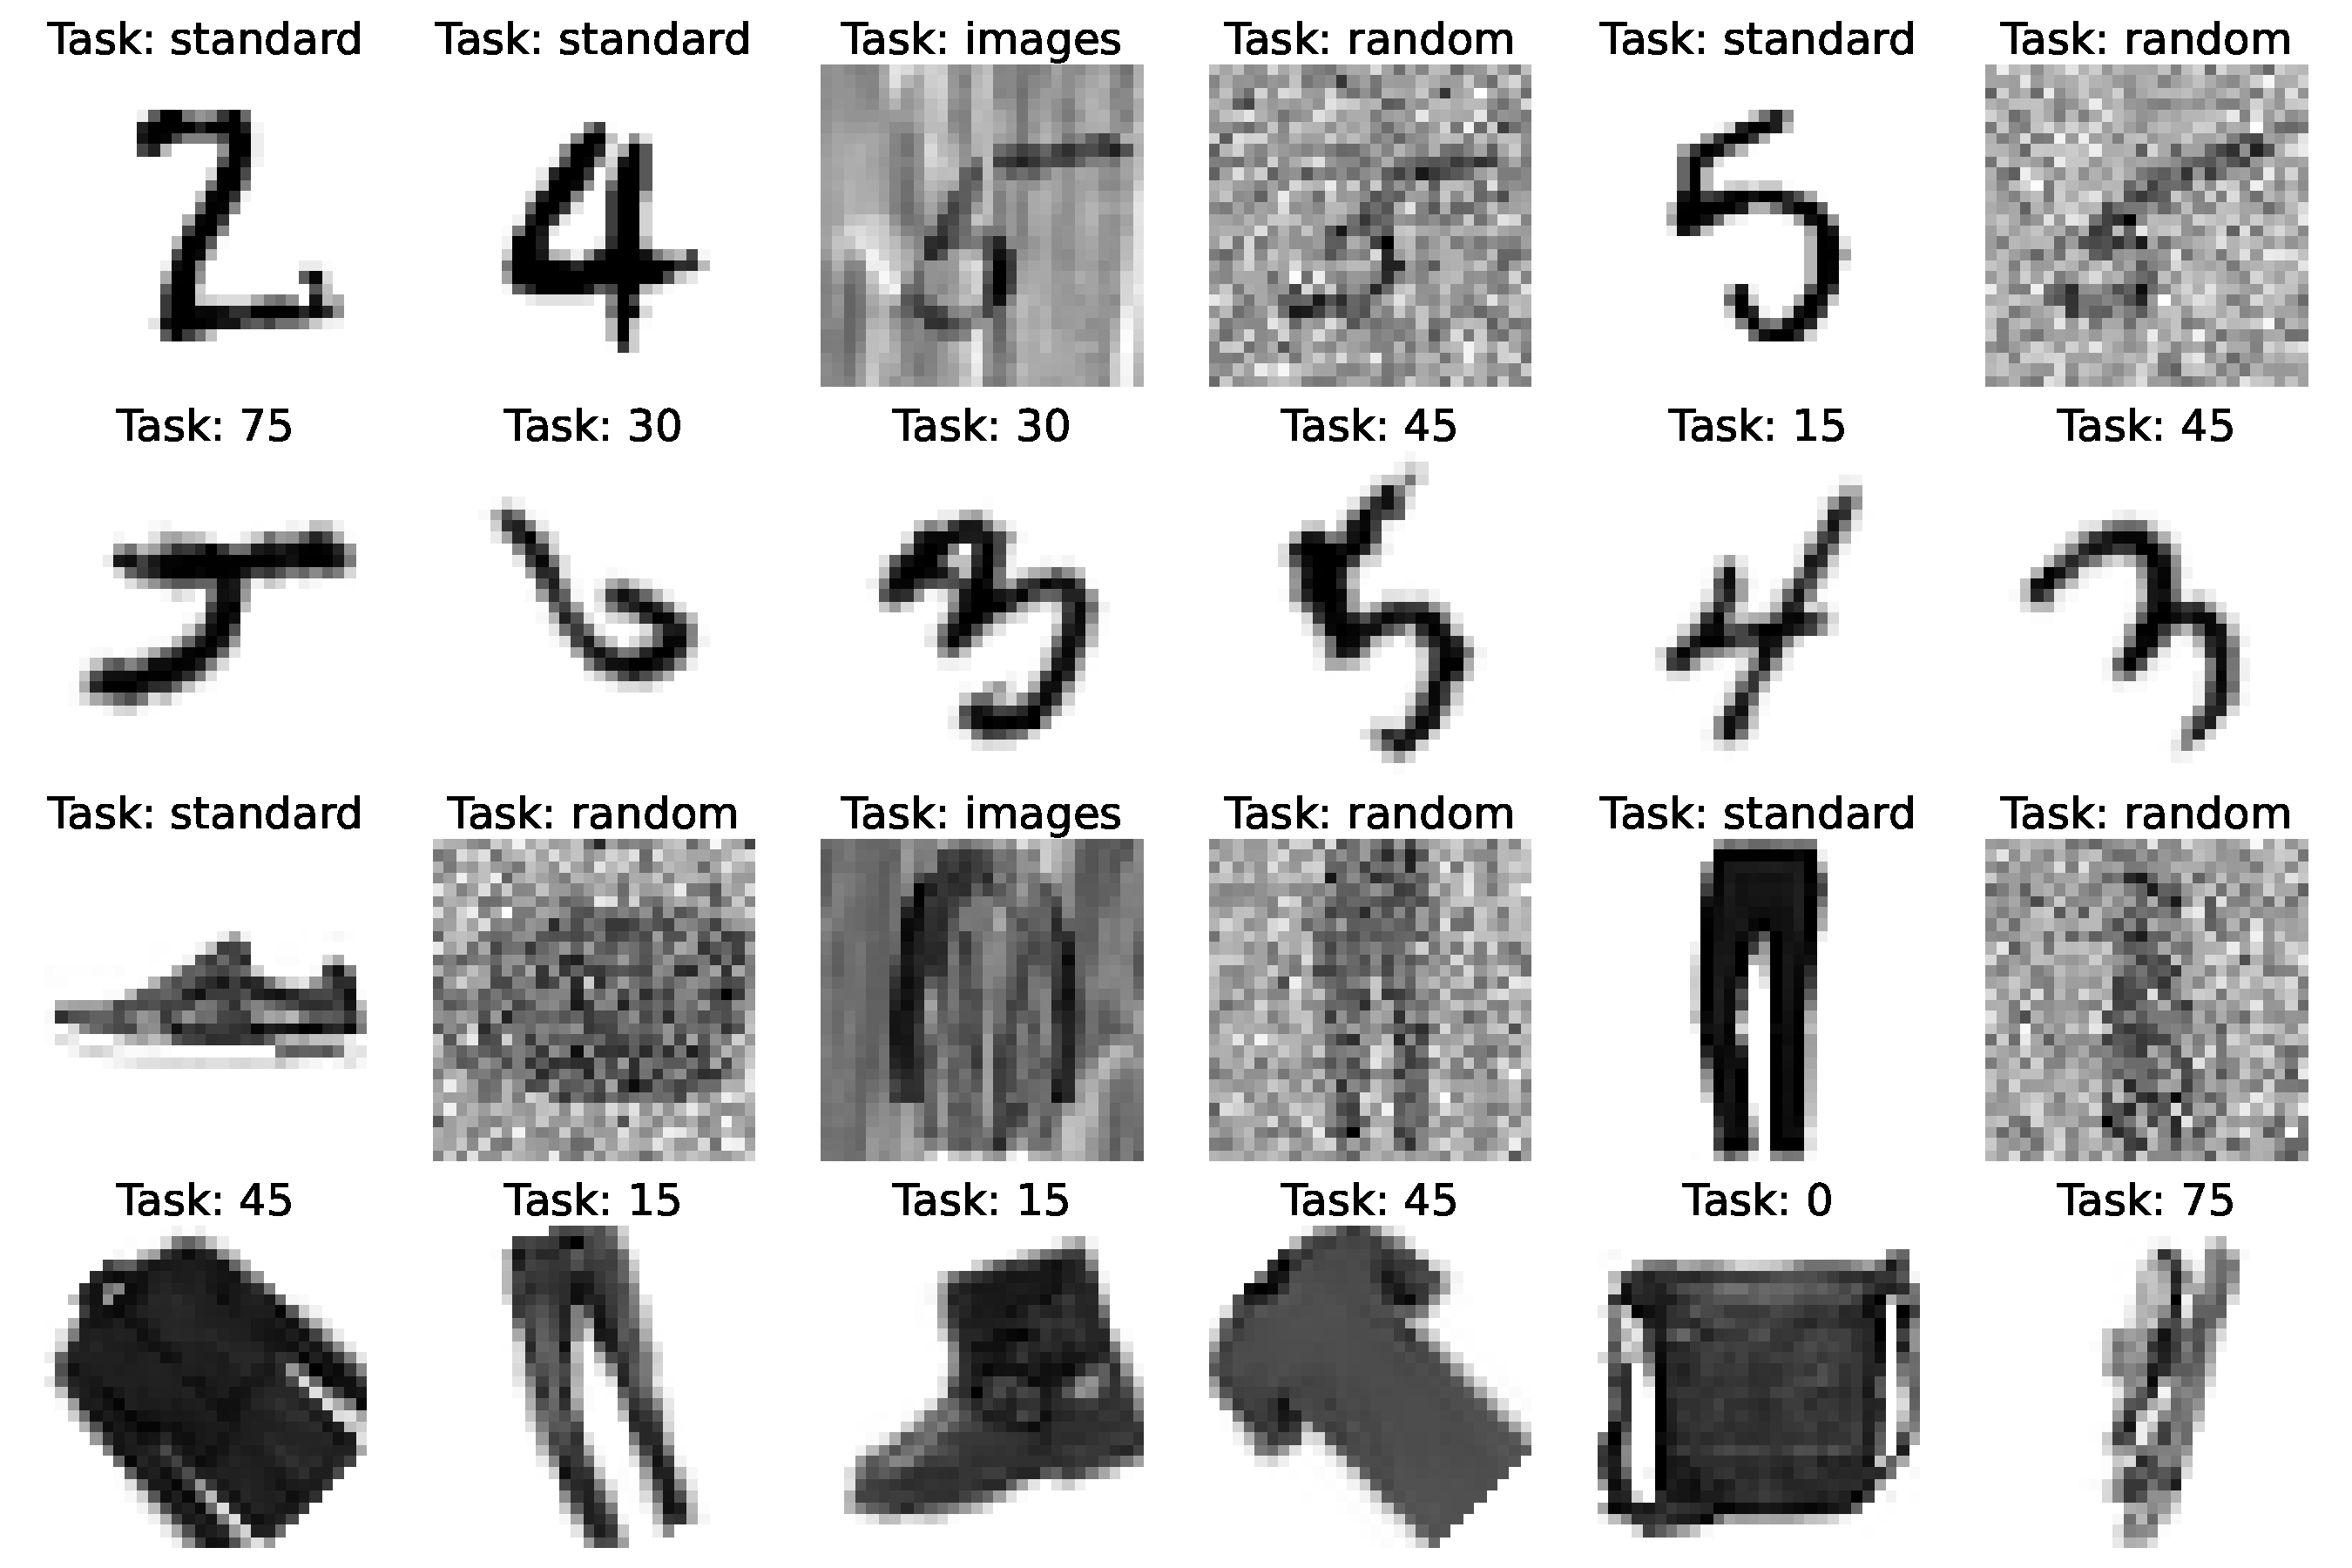
\includegraphics[width=.7\linewidth]{Chapter6/HAIS2022/hais22_datasets.pdf}

\end{frame}

\begin{frame}{Models}

      \begin{itemize}
          \item Comparamos cuatro modelos:
          \begin{itemize}
              \item \fmod{ctlNN\_conv}
              \item \fmod{itlNN\_conv}
              \item \fmod{cvxmtlNN\_conv}
              \item \fmod{hsmtlNN\_conv}
          \end{itemize}
          \item Todos están basados en una red convolucional de \texttt{Pytorch} con
          \begin{itemize}
              \item Conv. Layer (10 output channels)
              \item Conv. Layer (20 output channels)
              \item Dropout ($p=0.5$) and Max. Pooling
              \item Fully Connected Layer (320 neurons)
              \item Fully Connected Layer (50 neurons)
          \end{itemize}
          \item Todos los modelos se entrenan con el algoritmo \emph{AdamW}
      \end{itemize}
  
  \end{frame}

% \begin{frame}
%       \frametitle{Resultados}
%       \centering
%       \scalebox{.9}{
%             \begin{tabular}{l*{4}{c}}
%                 \hline
%                                    &   \fdata{var-MNIST} &   \fdata{rot-MNIST} &   \fdata{var-FMNIST} &   \fdata{rot-FMNIST} \\
%                 \hline
%                  \fmod{ctlNN} &              0.964 &           0.973 &                     0.784 &                  0.834 \\
%                  \fmod{itlNN} &              0.968 &           0.981 &                     0.795 &                  0.873 \\
%                  \fmod{hsNN}  &              0.971 &           0.980  &                    0.770  &                 0.852 \\
%                  \multirow{2}*{\fmod{mtlNN}} &              \fmaxn{0.974} &           \fmaxn{0.984} &                     \fmaxn{0.812} &                  \fmaxn{0.880} \\
%                  & ($\lambda^* = {0.6}$)  & ($\lambda^* = {0.8}$) & ($\lambda^* = {0.6}$)  & ($\lambda^* = {0.6}$) \\
%                  \hline
%             \end{tabular}
%       }
% \end{frame}


\begin{frame}
      \frametitle{Resultados}
  
      % \begin{itemize}
      %     \item The accuracy test scores are computed using majority voting   
      %     \item The categorical cross-entropy test scores are computed using a combination of the outputs (of the $5$ refitted models) 
      % \end{itemize}
  
      \begin{table}[t!]
          \centering
              %\caption{Test Accuracy with Majority Voting.}
              \label{tab:test_accuracy_majority}
          \scalebox{0.9}{
          \begin{tabular}{l*{4}{c}}
              \hline
                                 &   \fdata{var-MNIST} &   \fdata{rot-MNIST} &   \fdata{var-FMNIST} &   \fdata{rot-FMNIST} \\
              \hline
              & \multicolumn{4}{c}{accuracy} \\
              \hline
               \fmod{ctlNN} &              0.964 &           0.973 &                     0.784 &                  0.834 \\
               \fmod{itlNN} &              0.968 &           0.981 &                     0.795 &                  0.873 \\
               \fmod{hsmtlNN}  &              0.971 &           0.980  &                    0.770  &                 0.852 \\
               \multirow{2}*{\fmod{cvxmtlNN}} &              \fmaxn{0.974} &           \fmaxn{0.984} &                     \fmaxn{0.812} &                  \fmaxn{0.880} \\
               & ($\lambda^* = {0.6}$)  & ($\lambda^* = {0.8}$) & ($\lambda^* = {0.6}$)  & ($\lambda^* = {0.6}$) \\
               \hline
               & \multicolumn{4}{c}{categorical cross-entropy} \\
              \hline
               \fmod{ctlNN} & 1.274 $\pm$ 0.143  & 1.145 $\pm$ 0.039 & 2.369 $\pm$ 0.183         & 1.757 $\pm$ 0.075      \\
               \fmod{itlNN} & 1.072 $\pm$ 0.029  & 0.873 $\pm$ 0.058 & 2.356 $\pm$ 0.130         & 1.598 $\pm$ 0.042      \\
               \fmod{hsmtlNN}  & 1.087 $\pm$ 0.253  & 0.898 $\pm$ 0.073 & 3.067 $\pm$ 0.888         & 1.888 $\pm$ 0.075      \\
               \multirow{2}*{\fmod{cvxmtlNN}} & \fmaxn{0.924} $\pm$ \fmaxn{0.024}  & \fmaxn{0.831} $\pm$ \fmaxn{0.029} & \fmaxn{2.147} $\pm$ \fmaxn{0.090}         & \fmaxn{1.482} $\pm$ \fmaxn{0.063}      \\
               & ($\lambda^* = {0.6}$)  & ($\lambda^* = {0.8}$) & ($\lambda^* = {0.6}$)  & ($\lambda^* = {0.6}$)      \\
               \hline
              \end{tabular}
          }
      \end{table}
  
  \end{frame}




%%%%%%%%%%%%%%%%%%%%%%%%%%%%%%%%%%%%%%%%%%%%%%%%%%%%%%%%%%%%%%%%%%%%%%%%%%%%%%%%%%%%%%%%
\section{Laplaciano Adaptativo para Aprendizaje Multitarea}

\begin{frame}
      \frametitle{Aprendizaje Multitarea con Regularización Laplaciana}

      \begin{itemize}
            \item Otra manera de acoplar distintas tareas es usar una regularización Laplaciana
            \item Consideramos un grafo donde
            \begin{itemize}
                  \item Los nodos representan tareas
                  \item Las aristas y sus pesos representan las relaciones entre las tareas
            \end{itemize}
            \item La matriz de adyacencia $A$ tiene los pesos de las aristas
            \item La matriz de grados $D$ es una matriz diagonal donde
            $$ (D)_{rr} = \sum_{s=1}^\ntasks (A)_{rs}$$
            \item La matriz Laplaciana se define como $L = D - A$
      \end{itemize}
      
\end{frame}


\begin{frame}
      \frametitle{Aprendizaje Multitarea con Regularización Laplaciana}

      \begin{itemize}
            \item Dados los modelos para cada tarea definidos como
            $$ \hypf_r(\cdot) = \dotp{w_r}{\cdot} + b_r$$
            \item Definimos la regularización
            \begin{equation}
                  \nonumber
                  %\label{eq:gl_regularization}
                  \sum_{r=1}^\ntasks \sum_{s=1}^\ntasks (A)_{rs} \norm{w_r - w_s}^2 ,
              \end{equation}
            \item Esta regularización se puede expresar como
            \begin{equation}
                  \nonumber
                  %\label{eq:gl_regularization}
                  \sum_{r=1}^\ntasks \sum_{s=1}^\ntasks (A)_{rs} \norm{w_r - w_s}^2 = \sum_{r=1}^\ntasks \sum_{s=1}^\ntasks (L)_{rs} \dotp{w_r}{w_s} ,
              \end{equation}
      \end{itemize}
      
\end{frame}




\subsection{Laplaciano de Grafo con Métodos de Kernel}

\begin{frame}
      \frametitle{Laplaciano de Grafo con Métodos de Kernel}

      \begin{itemize}
            % \item La regularización Laplaciana penaliza las distancias
            % \item ¿Cómo calcular las distancias en un Espacio de Hilbert con Kernel Reproductor?
            \item Consideramos el problema de minimización
            \begin{equation}
                  \label{eq:mtl_kernel_altext_original}
                  \begin{aligned}
                       & R({u_1, \ldots, u_T}) = \sum_{r=1}^{\ntasks} \sum_{i=1}^{\npertask_r} \lossf(y_i^r, \dotp{u_r}{\phi(x_i^r)}) + \mu \sum_r \sum_s (E)_{rs} \dotp{u_r}{u_s}  \\
                  \end{aligned}
            \end{equation}
            \item Si usamos el vector $\fv{u}^\intercal = (u_1^\intercal, \ldots, u_\ntasks^\intercal)$ lo expresamos como
            \begin{equation}
                  \label{eq:mtl_kernel_altext_tensor}
                  \begin{aligned}
                          & R(\myvec{u}) = \sum_{r=1}^{\ntasks} \sum_{i=1}^{\npertask_r} \lossf(y_i^r, \dotp{\myvec{u}}{e_r \otimes \phi(x_i^r)}) + \mu \left(  \myvec{u}^\intercal (E \otimes I) \myvec{u} \right) \\
                  \end{aligned}
              \end{equation}
              donde $\otimes$ indica el producto tensorial y $e_1, \ldots e_\ntasks$ es la base canónica de $\reals^\ntasks$
      \end{itemize}

\end{frame}

\begin{frame}
      \frametitle{Laplaciano de Grafo con Métodos de Kernel}

      \begin{lemma}\label{lemma:regproblems_kernel}
            Las soluciones $u_1^*, \ldots, u_\ntasks^*$ de~\eqref{eq:mtl_kernel_altext_original}, o equivalentemente la solución $\opt{\fv{u}}$ de~\eqref{eq:mtl_kernel_altext_tensor},    
            se pueden obtener minimizando
            \begin{equation}
                \label{eq:mtl_kernel_tensor}
                \begin{aligned}
                     & S(\myvec{w}) = \sum_{r=1}^{\ntasks} \sum_{i=1}^{\npertask_r} \lossf(y_i^r, \dotp{\myvec{w}}{(B_r \otimes \phi(x_i^r))}) + \mu  \myvec{w}^\intercal \myvec{w} , \\
                \end{aligned}
            \end{equation}
            donde $\bm{w} \in \reals^p \otimes \hilbertspace$ con $p \geq \ntasks$ y $B_r$ son las columnas de $B \in \reals^{p \times \ntasks}$, una matriz de rango máximo tal que $\mymat{E}^{-1} = \mymat{B}^\intercal \mymat{B}$.
        \end{lemma}
        El kernel reproductor correspondiente es:
        \begin{equation}
            \nonumber
            \dotp{B_r \otimes \phi(x_i^r)}{B_s \otimes \phi(x_j^s)} = \left(E^{-1} \right)_{rs} k(x_i^r, x_j^s) 
        \end{equation}

\end{frame}


\begin{frame}
      \frametitle{Laplaciano de Grafo con Métodos de Kernel y Formulación Convexa}
      \begin{itemize}
            \item Propuesta: combinar la formulación convexa con la regularización Laplaciana
            \item El problema de minimización es
            \begin{equation}
                  \nonumber%\label{eq:mtl_kernel_altext_original}
                  \begin{aligned}
                       & \sum_{r=1}^{\ntasks} \sum_{i=1}^{\npertask_r} \lossf(y_i^r, \lambda_r \dotp{w}{\phi(x_i^r)} + (1- \lambda_r) \dotp{ v_r}{\phi(x_i^r)}) \\
                       &\quad + \mu \sum_r \sum_s (L)_{rs} \dotp{v_r}{v_s} + \sum_{r=1}^\ntasks \dotp{v_r}{v_r} + \dotp{w}{w} \\
                  \end{aligned}
            \end{equation}
            \item Usando esta formulación y el lema anterior proponemos:
            \begin{itemize}
                  \item L1-SVM MT convexa con regularización laplaciana
                  \item L2-SVM MT convexa con regularización laplaciana
                  \item LS-SVM MT convexa con regularización laplaciana
            \end{itemize}
            
      \end{itemize}
      

\end{frame}

\begin{frame}
      \frametitle{Formulación Convexa para L1-SVM MT con Laplaciano}
  
      \begin{block}{Problema Primal - L1-SVM Convexa con Laplaciano}
            \begin{equation}\nonumber
                  \begin{aligned}
                       & \min_{\fv{v}, \fv{b}, \fv{\xi}, w}
                       &                                             & { C \sum_{r=1}^\ntasks \sum_{i=1}^{\npertask_r} {\xi_i^r}  + \frac{\nu}{2} \sum_{r=1}^\ntasks \sum_{s=1}^T (L)_{rs} \dotp{v_r}{v_s} + \frac{1}{2} \sum_r \norm{{v}_r}^2 + \frac{1}{2} \norm{{w}}^2}                                                                              \\
                       & \text{s.t.}
                       &                                             & y_i^r (\lambda_r (\dotp{w}{\phi({x}_i^r)}) + (1 - \lambda_r) (\dotp{{v}_r}{\psi({x}_i^r})) + b_r) \geq p_i^r - \xi_i^r  ,                                                                                                                                                                            \\
                       &                                             &                                                                                                                                                                                                           & \xi_i^r \geq 0,  \;  i = 1, \dotsc, \npertask_r, \; r=1, \dotsc, \ntasks .
                  \end{aligned}
              \end{equation}
      \end{block}
      \begin{itemize}
            \item Los hiperparámetros $\lambda_r$ regulan la influencia de cada parte:
            \begin{itemize}
                \item $\lambda_1, \ldots, \lambda_\ntasks=0$: modelos independientes (ITL)
                \item $\lambda_1, \ldots, \lambda_\ntasks=1$: modelo común (CTL)
            \end{itemize}
            \item La matriz laplaciana $L$ establece relaciones entre las partes específicas $v_r$
      \end{itemize}

\end{frame}


\begin{frame}
      \frametitle{Formulación Convexa para L1-SVM MT con Laplaciano}
  
      \begin{block}{Problema Dual - L1-SVM Convexa con Laplaciano}
            \begin{equation}\nonumber%\label{eq:dual_cvxgl_l1_kernel}
                  \begin{aligned}
                       & \min_{\fv{\alpha}}
                       &                       & \Theta(\fv{\alpha}) = \frac{1}{2} \fv{\alpha}^t \left( \Lambda \fm{Q} \Lambda + \left(\fm{I}_{\nsamples} - \Lambda \right) \fm{\widetilde{Q}} \left(\fm{I}_{\nsamples} - \Lambda \right) \right) \fv{\alpha} - \fv{p} \fv{\alpha}                                                             \\
                       & \text{s.t.}
                       &                       & 0 \leq \alpha_i^r \leq C, \;  i=1,\ldots,m_r, r=1,\ldots,T ,                                                                                                                                                                                                                                  \\
                       &                       &                                                                                                                                                                                                                                   & \sum_{i=1}^{n_r}{\alpha_i^r y_i^r} = 0, \; r=1,\ldots,T .
                  \end{aligned}
              \end{equation}
      \end{block}
      \begin{itemize}
            \item Usamos la matriz $  \Lambda = \Diag(\overbrace{\lambda_1, \ldots, \lambda_1}^{\npertask_1}, \ldots, \overbrace{\lambda_\ntasks, \ldots, \lambda_\ntasks}^{\npertask_\ntasks}) $
            \item La matriz $Q$ es común entre todas las tareas usando el kernel $k_\phi$ correspondiente a $\phi$
            \item La matriz $\tilde{Q}$ se define usando el kernel: $\widetilde{k}_\psi(x_i^r, x_j^s) = \left( \left(\nu \fm{L} + \fm{I}_\ntasks\right)^{-1} \right)_{rs} k_\psi(x_i^r, x_j^s) $
            % \begin{equation}
            %       \label{eq:kernelfun_gl_kernel}
            %       \widetilde{k}(x_i^r, x_j^s) = \left( \left(\nu \fm{L} + \fm{I}_\ntasks\right)^{-1} \right)_{rs} k(x_i^r, x_j^s) ,
            %   \end{equation}
            \item La función de kernel es: 
            $    \widehat{k}({x}_i^r, {x}_j^s) = \lambda_r \lambda_s k_\phi({x}_i^r, {x}_j^s) +  (1-\lambda_r) (1 - \lambda_s) \widetilde{k}_\psi({x}_i^r, {x}_j^s) 
            $
      \end{itemize}

\end{frame}


\begin{frame}
      \frametitle{Formulación Convexa para L2-SVM MT con Laplaciano}
  
      \begin{block}{Problema Primal - L2-SVM Convexa con Laplaciano}
            \begin{equation}\nonumber
                  \begin{aligned}
                       & \min_{\substack{v_1, \ldots, v_\ntasks ;                                                                                                                                                                                                                                                                                          \\ \substack{b_1, \ldots, b_\ntasks } ; \\ \substack{\fv{\xi}}, w; }}
                       &                                             & { C \sum_{r=1}^\ntasks \sum_{i=1}^{\npertask_r} {(\xi_i^r)^2}  + \frac{\nu}{2} \sum_{r=1}^\ntasks \sum_{s=1}^T (A)_{rs} {\| {v}_r - {v}_s \|}^2 + \frac{1}{2} \sum_r \norm{{v}_r}^2 + \frac{1}{2} \norm{{w}}^2}                                                                              \\
                       & \text{s.t.}
                       &                                             & y_i^r (\lambda_r (\dotp{w}{\phi({x}_i^r)}) + (1 - \lambda_r) (\dotp{{v}_r}{\psi({x}_i^r})) + b_r) \geq p_i^r - \xi_i^r  ;
                  \end{aligned}
              \end{equation}
      \end{block}
      \begin{block}{Problema Dual - L2-SVM Convexa con Laplaciano}
            \begin{equation}\nonumber
                  \begin{aligned}
                       & \min_{\fv{\alpha}}
                       &                       & \Theta(\fv{\alpha}) = \frac{1}{2} \fv{\alpha}^t \left\lbrace  \left( \Lambda \fm{Q} \Lambda + \left(\fm{I}_{\nsamples} - \Lambda \right) \fm{\widetilde{Q}} \left(\fm{I}_{\nsamples} - \Lambda \right) \right) + \frac{1}{C} \fm{I}_\nsamples \right\rbrace \fv{\alpha} - \fv{p} \fv{\alpha}                                                            \\
                       & \text{s.t.}
                       &                       & 0 \leq \alpha_i^r, \;  i=1,\ldots,m_r,\; r=1,\ldots,T ,                                                                                                                                                                                                                                                                                                   \\
                       &                       &                                                                                                                                                                                                                                                                                              & \sum_{i=1}^{n_r}{\alpha_i^r y_i^r} = 0, \; r=1,\ldots,T.
                  \end{aligned}
              \end{equation}
      \end{block}
      

\end{frame}

\begin{frame}
      \frametitle{Formulación Convexa para LS-SVM MT con Laplaciano}
  
      \begin{block}{Problema Primal - LS-SVM Convexa con Laplaciano}
            \begin{equation}\nonumber
                  \begin{aligned}
                       & \min_{\substack{v_1, \ldots, v_\ntasks ;                                                                                                                                                                                                                                                                                          \\ \substack{b_1, \ldots, b_\ntasks } ; \\ \substack{\fv{\xi}}, w; }}
                       &                                             & { C \sum_{r=1}^\ntasks \sum_{i=1}^{\npertask_r} {(\xi_i^r)^2}  + \frac{\nu}{2} \sum_{r=1}^\ntasks \sum_{s=1}^T (A)_{rs} {\| {v}_r - {v}_s \|}^2 + \frac{1}{2} \sum_r \norm{{v}_r}^2 + \frac{1}{2} \norm{{w}}^2}                                                                              \\
                       & \text{s.t.}
                       &                                             & y_i^r (\lambda_r (\dotp{w}{\phi({x}_i^r)}) + (1 - \lambda_r) (\dotp{{v}_r}{\psi({x}_i^r})) + b_r) = p_i^r - \xi_i^r  ;
                  \end{aligned}
              \end{equation}
      \end{block}
      \begin{block}{Problema Dual - LS-SVM Convexa con Laplaciano}
            \begin{equation}\label{eq:dual_cvxgl_ls_kernel}
                  \begin{aligned}
                      \left[
                          \begin{array}{c|c}
                              \fm{0}_{\ntasks \times \ntasks} & \fm{A}^\intercal \fm{y}                                                                                                                                                         \\
                              \hline
                              \fm{y} \fm{A}                   & \left( \Lambda \fm{Q} \Lambda + \left(\fm{I}_{\nsamples} - \Lambda \right) \fm{\widetilde{Q}} \left(\fm{I}_{\nsamples} - \Lambda \right) \right) + \frac{1}{C} \fm{I}_\nsamples
                          \end{array}
                          \right]
                      \begin{bmatrix}
                          b_1       \\
                          \vdots    \\
                          b_\ntasks \\
                          \fv{\alpha}
                      \end{bmatrix}
                      =
                      \begin{bmatrix}
                          \fv{0}_\ntasks \\
                          \fv{p}
                      \end{bmatrix}.
                  \end{aligned}
              \end{equation}
      \end{block}
      

\end{frame}

\subsection{Algoritmo Adaptativo para Laplaciano de Grafo}

\begin{frame}
      \frametitle{Algoritmo Adaptativo para Laplaciano de Grafo}

      \begin{itemize}
            \item La selección de la matriz de adyacencia $A$ (y la respectiva $L$) determina la relación que se fomenta entre las tareas
            \item Tiene que tener las siguientes restricciones:
            \begin{itemize}
                  \item $A$ es simétrica
                  \item $(A)_{rs} \geq 0$, $r, s=1, \ldots, \ntasks$.
                  \item $\sum_{s=1} (A)_{rs} = 1$
              \end{itemize}
            %\item Se puede escoger usando conocimiento experto del problema
            %\item Proponemos un algoritmo para aprender la matriz $A$ de forma automática
            \item La entropía de cada fila es: $\fv{a}^r$: $H(\fv{a}^r) = \sum_{s=1}^\ntasks (A)_{rs} \log((A)_{rs})$
            \item Definimos la entropía de $A$ como: $H(A) = \sum_{r=1}^\ntasks H(\fv{a}^r)$
            \item Interpretación:
            \begin{itemize}
                  \item $H(A)$ es máxima si $A$ es constante, $A = \frac{1}{\ntasks} \fv{1}_\ntasks \fv{1}_\ntasks^\intercal$, 
                  \item $H(A)$ es mínima si $A$ es la identidad, $A = I_\ntasks$ 
            \end{itemize}
            
            % \item Proponemos un algoritmo para aprender la matriz de forma automática:
            % \begin{itemize}
            %       \item Empezamos con un enfoque agnóstico: $A$ constante
            %       \item Se calculan los parámetros $\opt{v_r}$ en cada tarea
            %       \item Se calculan las distancias entre tareas para determinar su relación
            %       \item Actualizamos la matriz $A$: $A_{rs} \propto \frac{1}{\norm{v_r - v_s}}$
            % \end{itemize}
      \end{itemize}

\end{frame}


\begin{frame}
      \frametitle{Algoritmo Adaptativo para Laplaciano de Grafo}

      \begin{block}{Problema para Algoritmo Adaptativo}
            \begin{equation}\nonumber %\label{eq:adapcvxgl_general_problem}
                  \begin{aligned}
                       & \min_{\substack{w, \fv{v}, \fv{b};                                                                                                                                                                                                                                                                                                                              \\  A \in {(\reals_{\geq 0})}^{\ntasks \times \ntasks},  \\ \fm{A} \fv{1}_\ntasks = \fv{1}_\ntasks}}
                       &                                       & C \sum_{r=1}^\ntasks \sum_{i=1}^{\npertask_r} {\lossf(\lambda_r \dotp{w}{\phi({x}_i^r)} + (1 - \lambda_r) \dotp{{v}_r}{\psi({x}_i^r)} + b_r, y_i^r)}                                                                                                                                                                       \\
                       &                                       &                                                                                                                                                      & \quad + \frac{\nu}{2} \sum_{r=1}^\ntasks \sum_{s=1}^\ntasks (A)_{rs} \norm{{v}_r - v_{s}}^2 + \frac{1}{2} \sum_{r=1}^\ntasks \norm{{v}_r}^2 + \frac{1}{2}\norm{{w}}^2 \\
                       &                                       &                                                                                                                                                      & \quad- \mu \sum_{r=1}^\ntasks H(\fv{a}^r) ,
                  \end{aligned}
              \end{equation}
            \end{block}

\end{frame}


\begin{frame}
      \frametitle{Algoritmo Adaptativo para Laplaciano de Grafo}

      \begin{itemize}
            \item Para minimizar este problema alternamos los siguientes pasos:
            \begin{itemize}
                  \item Fijamos $A$ y minimizamos en $w, \fv{v}, \fv{b}$: resolvemos el problema dual (y obtenemos $\opt{\fv{\alpha}}$) correspondiente a
                  \begin{equation}\nonumber %\label{eq:adapcvxgl_general_problem}
                        \begin{aligned}
                             & \min_{w, \fv{v}, \fv{b}}
                             &                                       & C \sum_{r=1}^\ntasks \sum_{i=1}^{\npertask_r} {\lossf(\lambda_r \dotp{w}{\phi({x}_i^r)} + (1 - \lambda_r) \dotp{{v}_r}{\psi({x}_i^r)} + b_r, y_i^r)}                                                                                                                                                                       \\
                             &                                       &                                                                                                                                                      & \quad + \frac{\nu}{2} \sum_{r=1}^\ntasks \sum_{s=1}^\ntasks (A)_{rs} \norm{{v}_r - v_{s}}^2 + \frac{1}{2} \sum_{r=1}^\ntasks \norm{{v}_r}^2 + \frac{1}{2}\norm{{w}}^2 
                        \end{aligned}
                    \end{equation}
                  % \begin{equation}\nonumber%\label{eq:dual_cvxgl_l1_kernel}
                  %       \begin{aligned}
                  %            & \min_{\fv{\alpha}}
                  %            &                       & \Theta(\fv{\alpha}) = \frac{1}{2} \fv{\alpha}^t \left( \Lambda \fm{Q} \Lambda + \left(\fm{I}_{\nsamples} - \Lambda \right) \fm{\widetilde{Q}} \left(\fm{I}_{\nsamples} - \Lambda \right) \right) \fv{\alpha} - \fv{p} \fv{\alpha}                                                             \\
                  %            & \text{s.t.}
                  %            &                       & 0 \leq \alpha_i^r \leq C, \;  i=1,\ldots,m_r, r=1,\ldots,T ,                                                                                                                                                                                                                                  \\
                  %            &                       &                                                                                                                                                                                                                                   & \sum_{i=1}^{n_r}{\alpha_i^r y_i^r} = 0, \; r=1,\ldots,T .
                  %       \end{aligned}
                  %   \end{equation}
                  \item Fjamos $w, \fv{v}, \fv{b}$ y minimizamos en $A$: 
                  \begin{equation}\nonumber
                        \begin{aligned}
                            \min_{\substack{A \in {(\reals_{\geq 0})}^{\ntasks \times \ntasks}, \\ \fm{A} \fv{1}_\ntasks = \fv{1}_\ntasks}}
                            J(A) = \frac{\nu}{2} \sum_{r=1}^\ntasks \sum_{s=1}^\ntasks (A)_{rs} \norm{{v}_r - v_{s}}^2 - \mu \sum_{r=1}^\ntasks H(\fv{a}^r) .
                        \end{aligned}
                    \end{equation}
            \end{itemize}
            
      \end{itemize}

\end{frame}

\begin{frame}
      \frametitle{Algoritmo Adaptativo para Laplaciano de Grafo}

      \begin{itemize}
            \item Si sabemos las distancias $\norm{v_r - v_s}^2$, la solución es
            \begin{equation}\nonumber%\label{eq:update_A}
                  (A)_{rs} = \frac{\exp{-\frac{\nu}{\mu} \norm{{v}_r - {v}_s}^2 } }{\sum_t \exp{-\frac{\nu}{\mu}  \norm{{v}_r - {v}_t}^2} } .
              \end{equation}
            \item ¿Cómo calculamos estas distancias?
            \begin{itemize}
                  \item Con la matriz $ \widetilde{{\fm{Q}^{rs}}}$ correspondiente a la función
            \begin{equation}
                  \nonumber%\label{eq:dot_computation_kernel}
                  \widetilde{{k^{rs}}}(x_i^t, x_j^\tau) = (\fm{I}_\ntasks + \nu \fm{L})^{-1}_{rt} (\fm{I}_\ntasks + \nu \fm{L})^{-1}_{s\tau} k_\psi(x_i^t, x_j^\tau) .
              \end{equation}
            \item Los productos interiores son
            \begin{equation}\nonumber%\label{eq:dot_computation_matrix}
                  \dotp{v_r}{v_s} = \fv{\alpha}^\intercal \left(\fm{I}_{\nsamples} - \Lambda \right) \widetilde{{\fm{Q}^{rs}}} \left(\fm{I}_{\nsamples} - \Lambda \right) \fv{\alpha} ,
              \end{equation}
              \item Las distancias son entonces
              \begin{equation}\nonumber%\label{eq:distance_computation_matrix}
                  \norm{v_r - v_s}^2 = \fv{\alpha}^\intercal \left(\fm{I}_{\nsamples} - \Lambda \right) (\widetilde{{\fm{Q}^{rr}}} + \widetilde{{\fm{Q}^{ss}}} - 2\widetilde{{\fm{Q}^{rs}}}) \left(\fm{I}_{\nsamples} - \Lambda \right) \fv{\alpha}.
              \end{equation}
            \end{itemize}     
      \end{itemize}

\end{frame}

\begin{frame}
      \frametitle{Algoritmo Adaptativo para Laplaciano de Grafo}

      \begin{algorithm}[H]
            \DontPrintSemicolon
            % \KwInput{$(X, y) = \set{(x_i^r, y_i^r), i=1, \ldots, \npertask_r; r=1, \ldots, \ntasks}$ \tcp*{Data}}
            % \KwOutput{$\fv{\alpha}^*$ \tcp*{Optimal dual coefficients}}
            % \KwOutput{$\fm{A}^*$ \tcp*{Optimal adjacency matrix}}
            % \KwData{params = $\set{C, \lambda, \nu, \mu, \sigma_\phi, \sigma_\psi (, \epsilon)}$ \tcp*{Hyperparameters}}
            %   $Q_\phi$ = ComputeKernelMatrix($(X, y)$, $\sigma_\phi$) \\
            %   $Q_\psi$ = ComputeKernelMatrix($(X, y)$, $\sigma_\psi$) \\
            %$o^\text{old}$ = $\infty$ \\
            $A = A_0$ \tcp*{Constant matrix}
            \While{True}{
                $L_\text{inv}$ $\gets$ getInvLaplacian($\fm{A}$) \tcp*{Step 0}
                $\alpha_\text{opt}$ $\gets$ solveDualProblem($(X, y)$, $L_\text{inv}$, params) \tcp*{Step 1}
                $o$ $\gets$ computeObjectiveValue($(X, y)$, $L_\text{inv}$, $\alpha_\text{opt}$) \tcp*{Objective function value}
                \If{$o^{old} - o \leq \delta_\text{tol}$}{break \tcp*{Exit condition}}
                %$o^{old} \gets o$ \\
                % \If{$J_\text{obj}^old - J_\text{obj} \geq \delta_\text{\tol}$}{
                %     break \\
                % }
                $D$ $\gets$ computeDistances($(X, y)$, $L_\text{inv}$, $\alpha_\text{opt}$) \tcp*{Step 2}
                $A$ $\gets$ updateAdjMatrix($D$, params) \tcp*{Step 3}
            }
            \Return{$\alpha_\text{opt}, A$}
            % \caption{Adaptive \acrshort{gl} algorithm.}
            % \label{alg:adapgl}
        \end{algorithm}
      % \begin{itemize}
      %       \item Step 0: invert the matrix $(I_\ntasks + \nu L)$
      %       \item Step 1: minimize the dual problem to obtain $\alpha^*$
      %       \item Step 2: compute the distances $\norm{v_r - v_s}^2$ between task parameters
      %       \item Step 3: update the adjacency matrix $A$ using~\eqref{eq:update_A}
      % \end{itemize}

\end{frame}


\begin{frame}
      \frametitle{Experimentos: Problemas Sintéticos}

      \begin{figure}
      \begin{subfigure}[b]{0.49\textwidth}
            \centering
            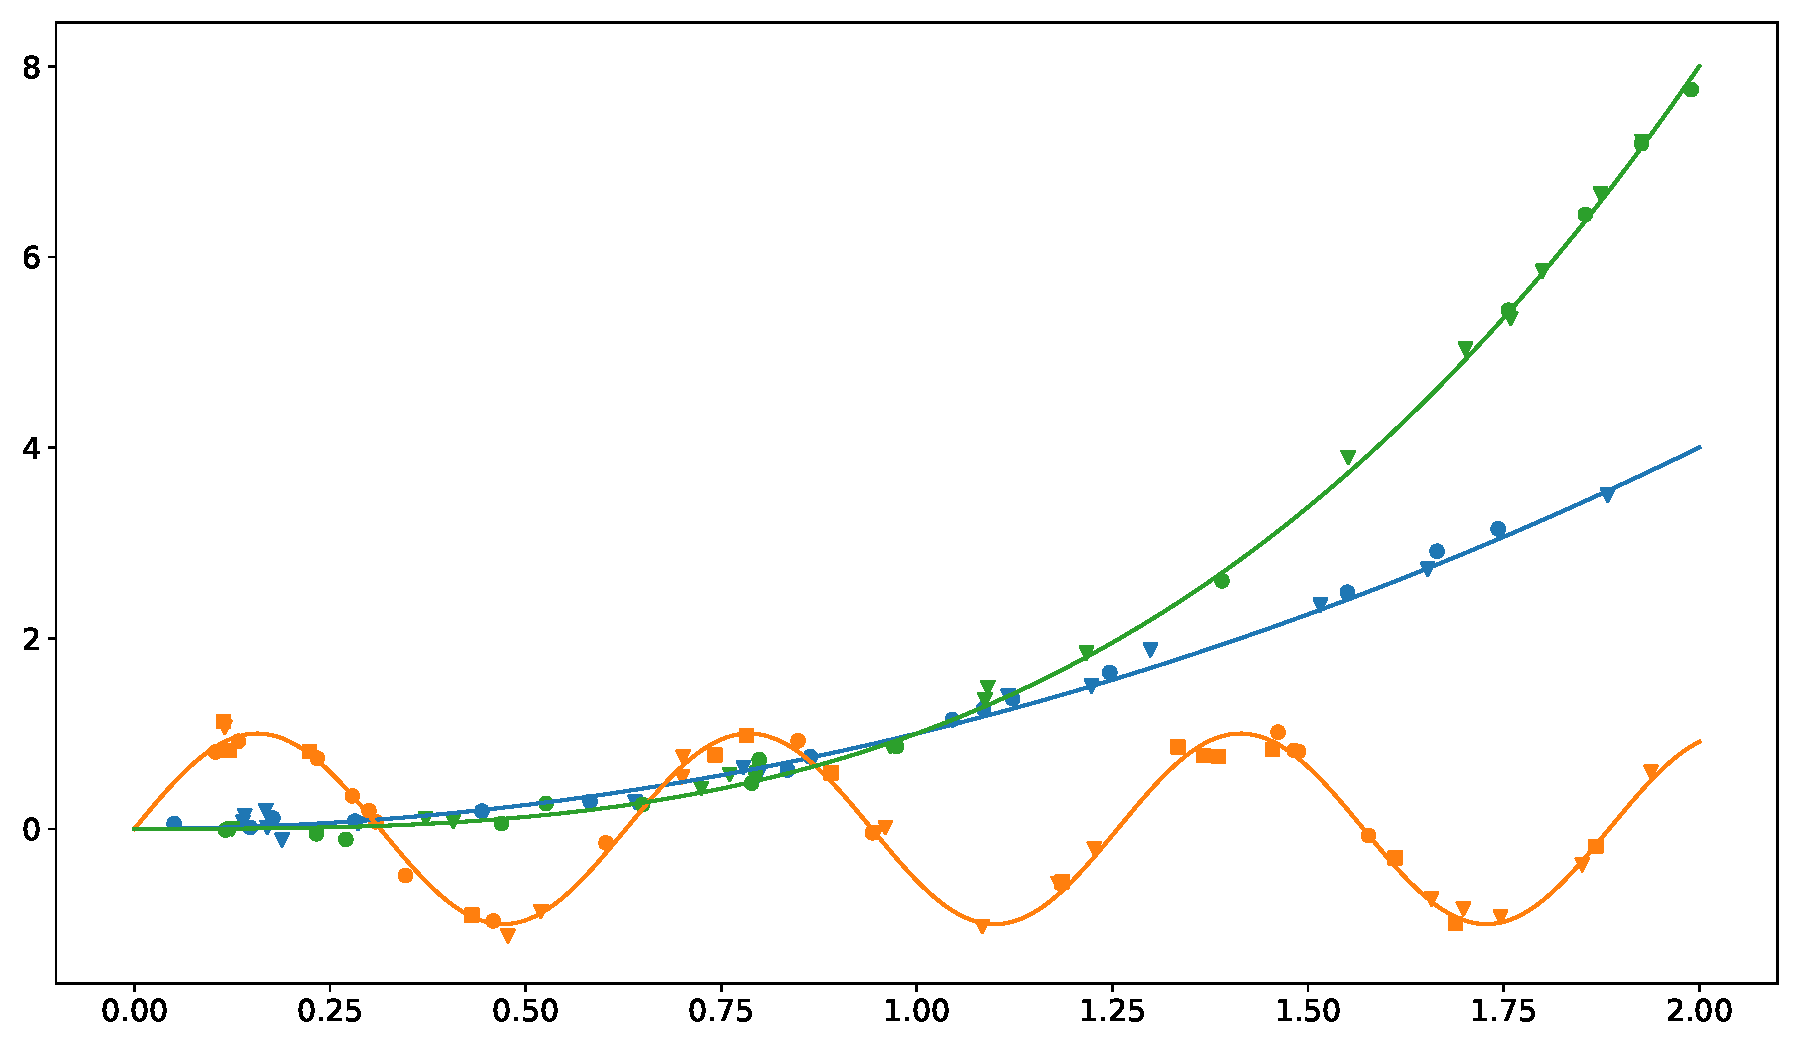
\includegraphics[width=\textwidth]{Chapter6/IGPL2022/regClusters__0.pdf}
            \caption{\fdata{regClusters0}.}
            % \label{regClusters0}
      \end{subfigure}
      \hfill
      \begin{subfigure}[b]{0.49\textwidth}
            \centering
            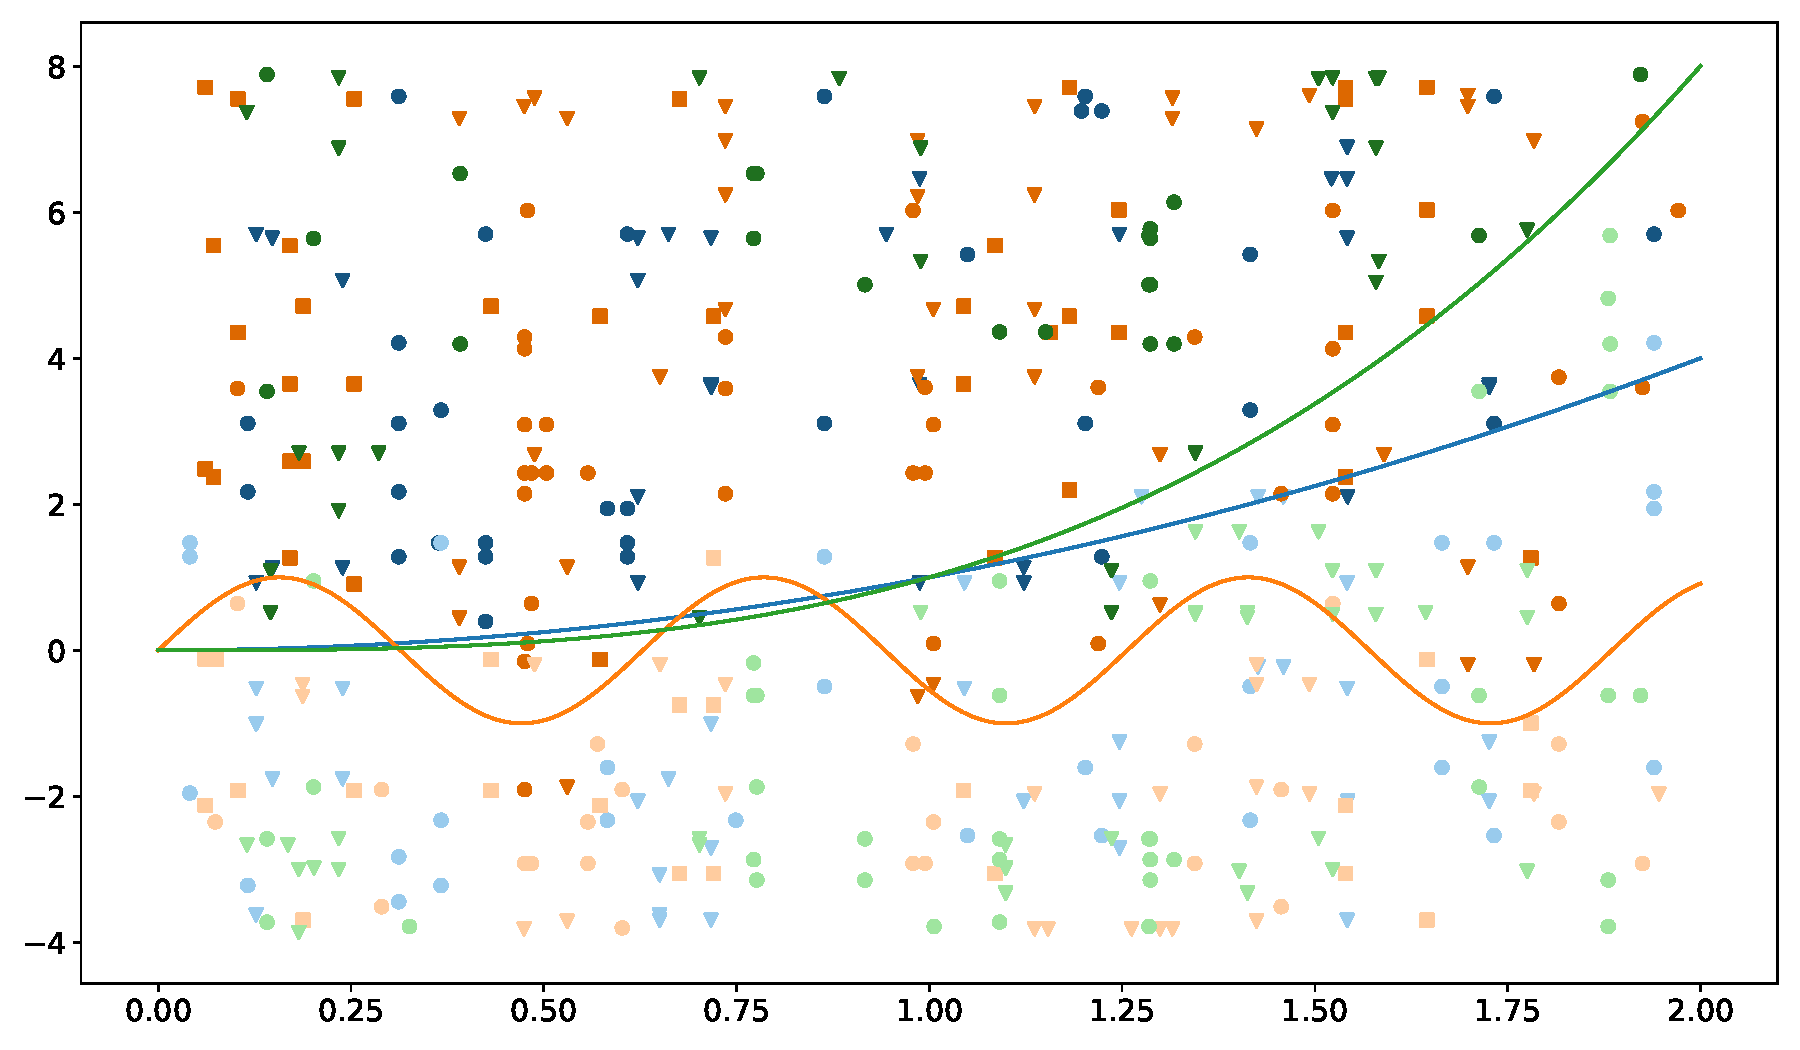
\includegraphics[width=\textwidth]{Chapter6/IGPL2022/clasClusters__0.pdf}
            \caption{\fdata{clasClusters0}.}
            %\label{clasClusters0}
      \end{subfigure}
      \end{figure}

\end{frame}

\begin{frame}
      \frametitle{Experimentos Sintéticos: Problemas}

      \begin{figure}
      \begin{subfigure}[b]{0.49\textwidth}
            \centering
            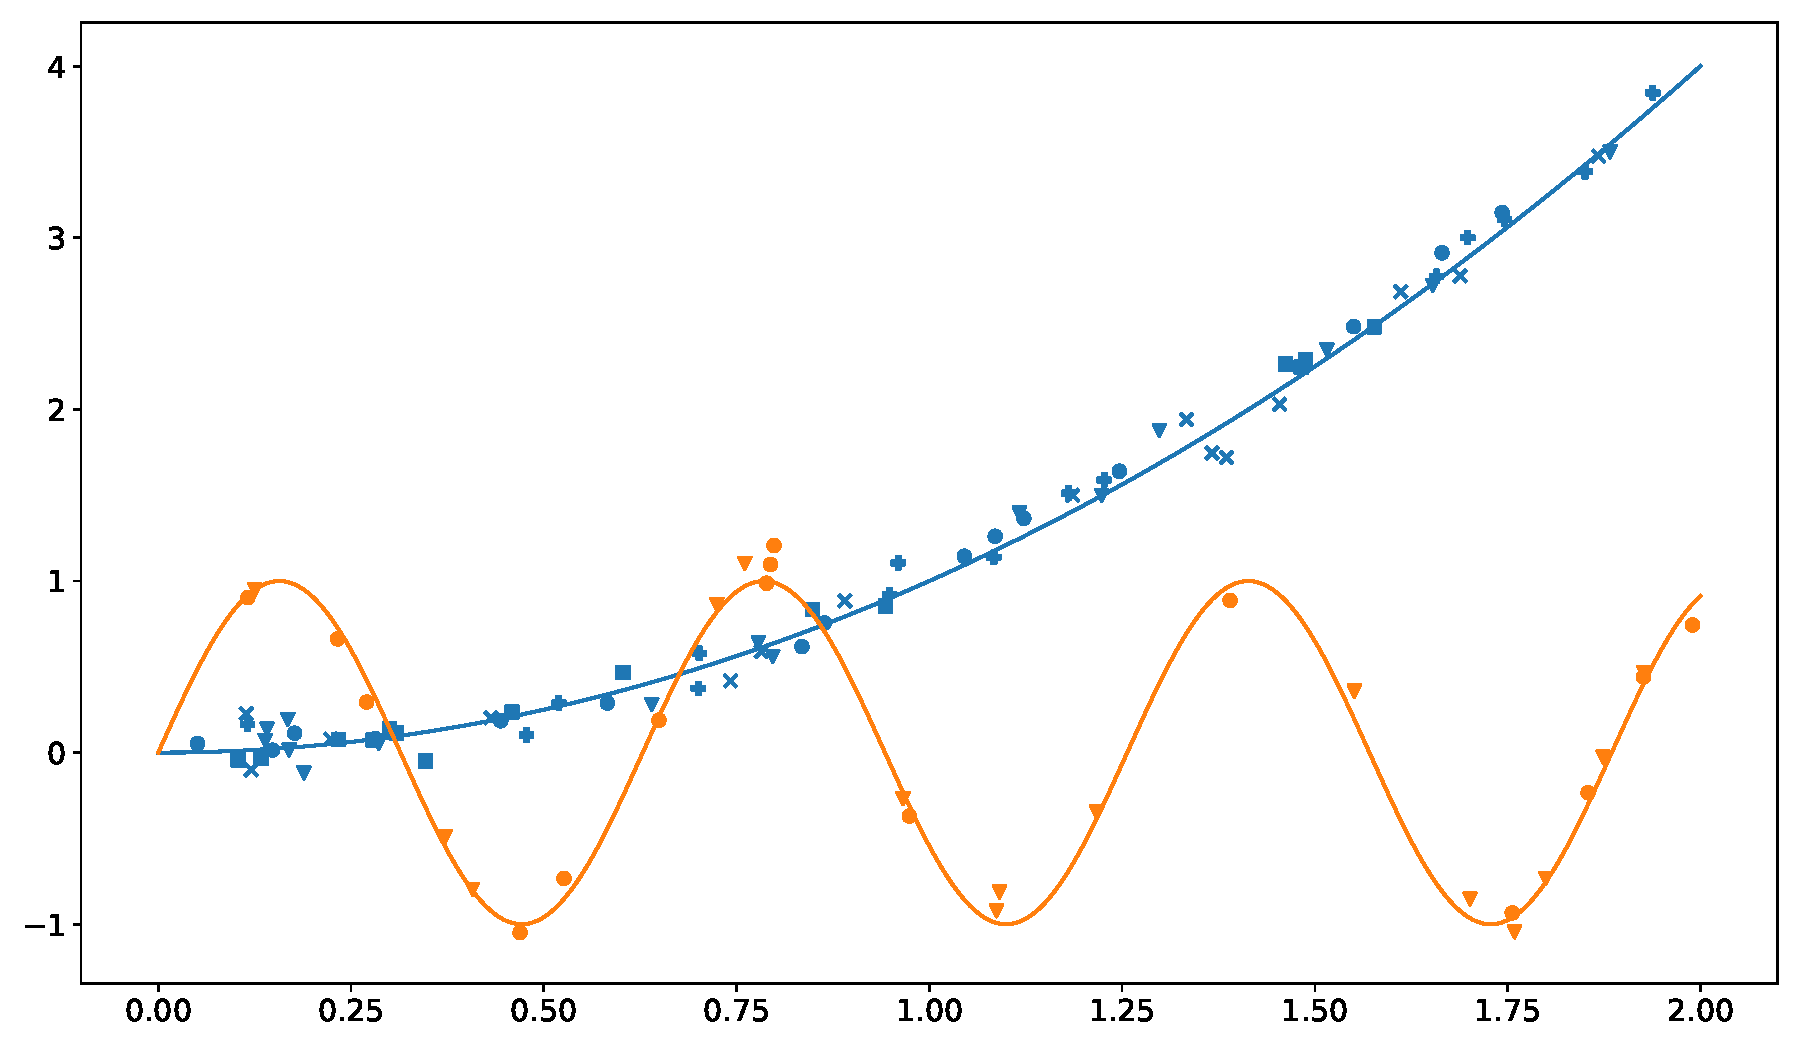
\includegraphics[width=\textwidth]{Chapter6/IGPL2022/regClusters__1.pdf}
            \caption{\fdata{regClusters1}.}
            % \label{regClusters0}
      \end{subfigure}
      \hfill
      \begin{subfigure}[b]{0.49\textwidth}
            \centering
            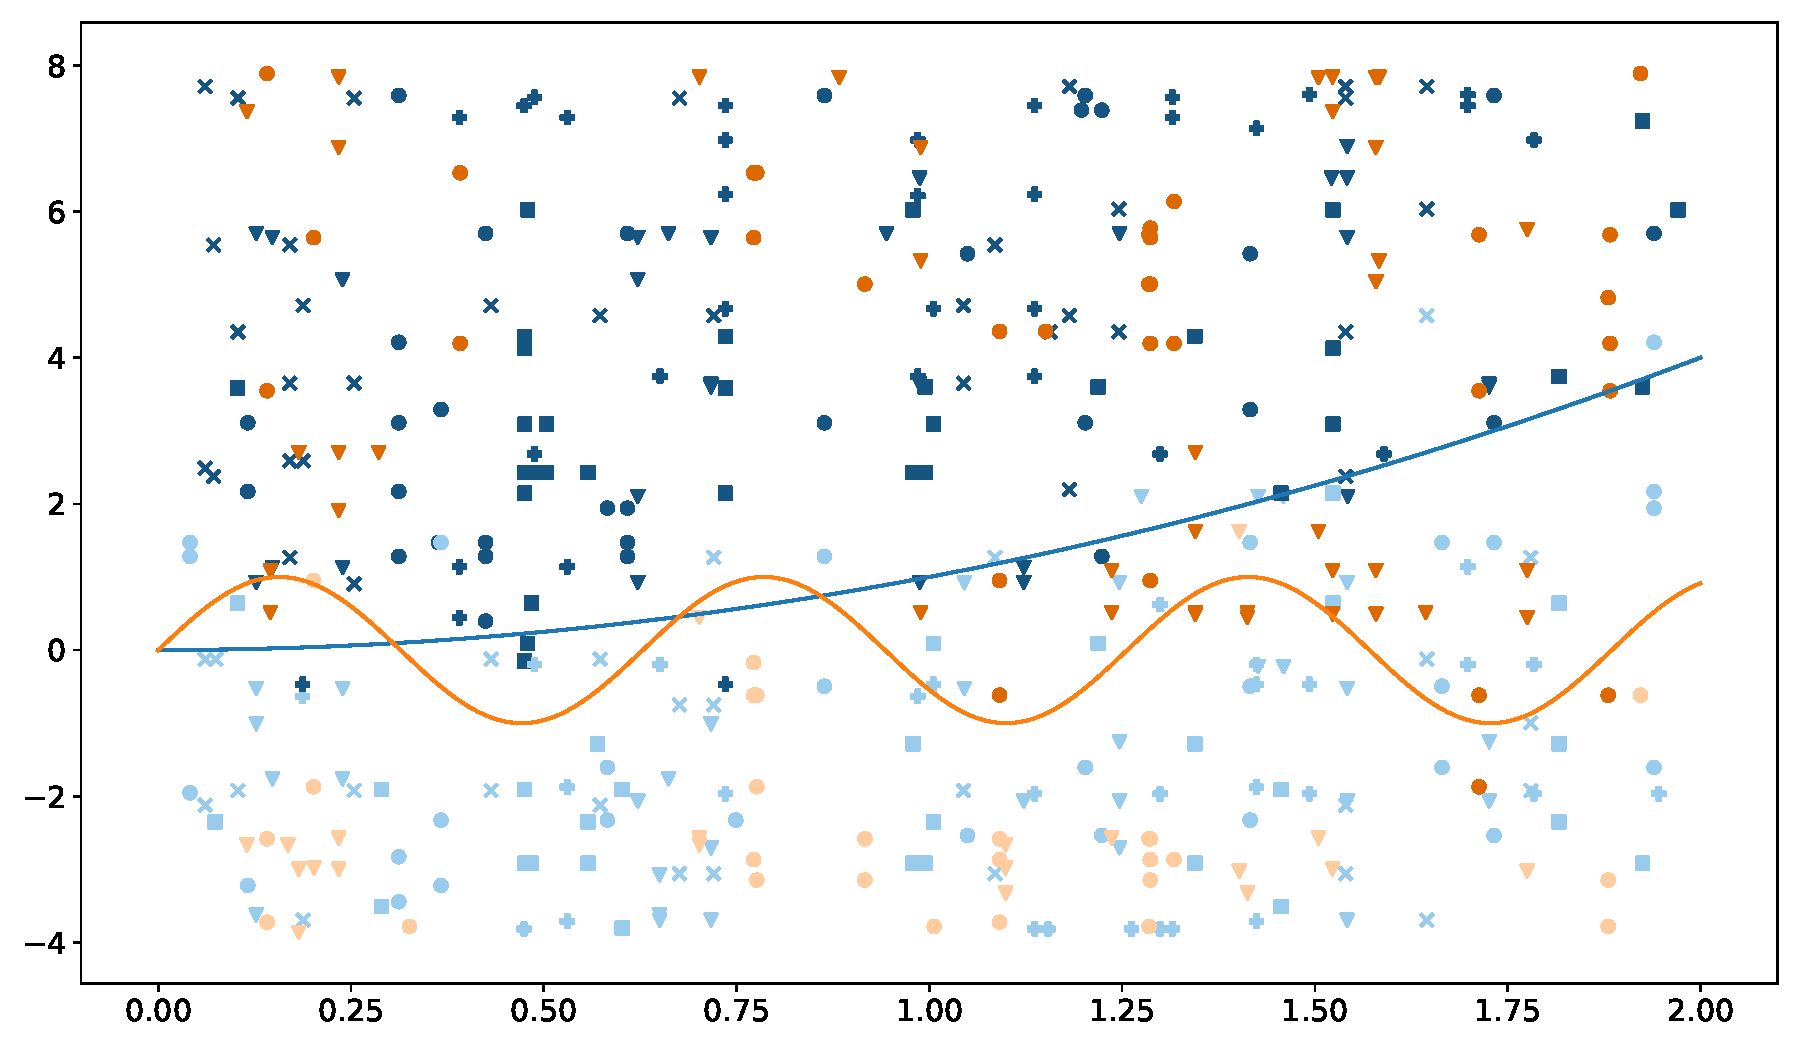
\includegraphics[width=\textwidth]{Chapter6/IGPL2022/clasClusters__1.pdf}
            \caption{\fdata{clasClusters1}.}
            %\label{clasClusters0}
      \end{subfigure}
      \end{figure}

\end{frame}

\begin{frame}
      \frametitle{Experimentos Sintéticos: Problemas Sintéticos}

      \begin{figure}
      \begin{subfigure}[b]{0.49\textwidth}
            \centering
            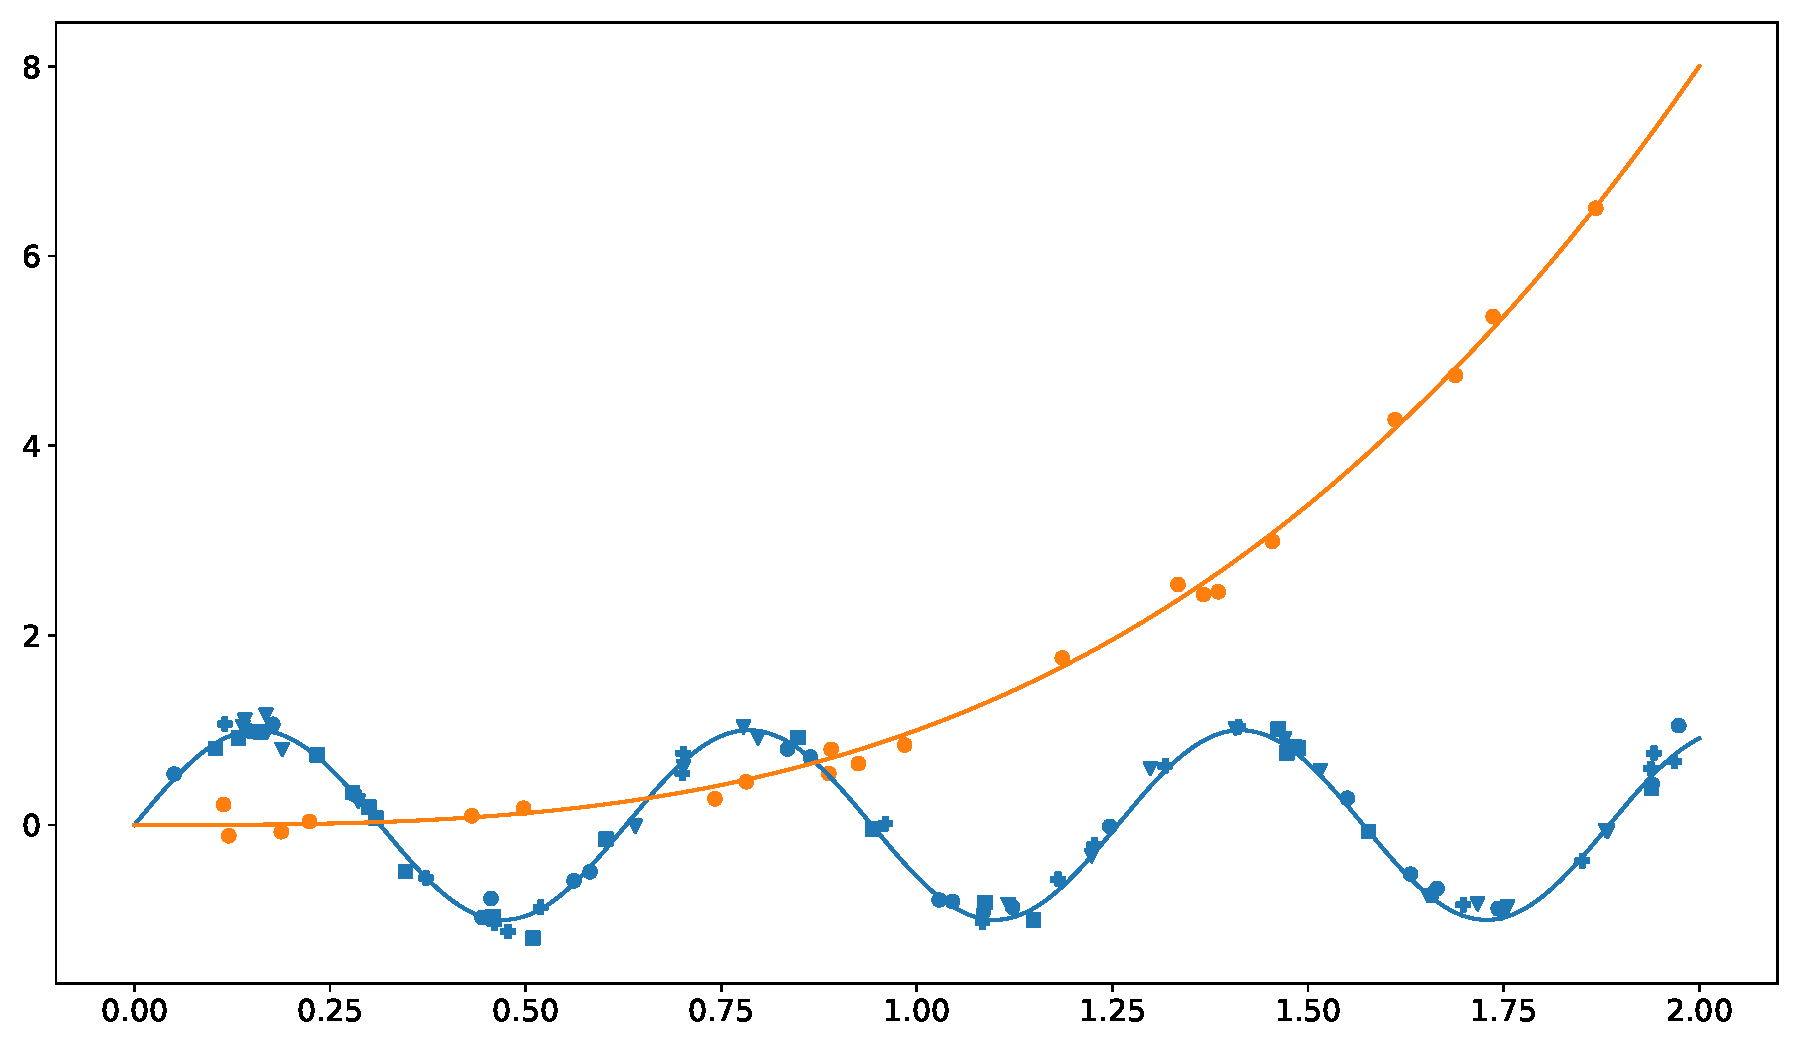
\includegraphics[width=\textwidth]{Chapter6/IGPL2022/regClusters__2.pdf}
            \caption{\fdata{regClusters2}.}
            % \label{regClusters0}
      \end{subfigure}
      \hfill
      \begin{subfigure}[b]{0.49\textwidth}
            \centering
            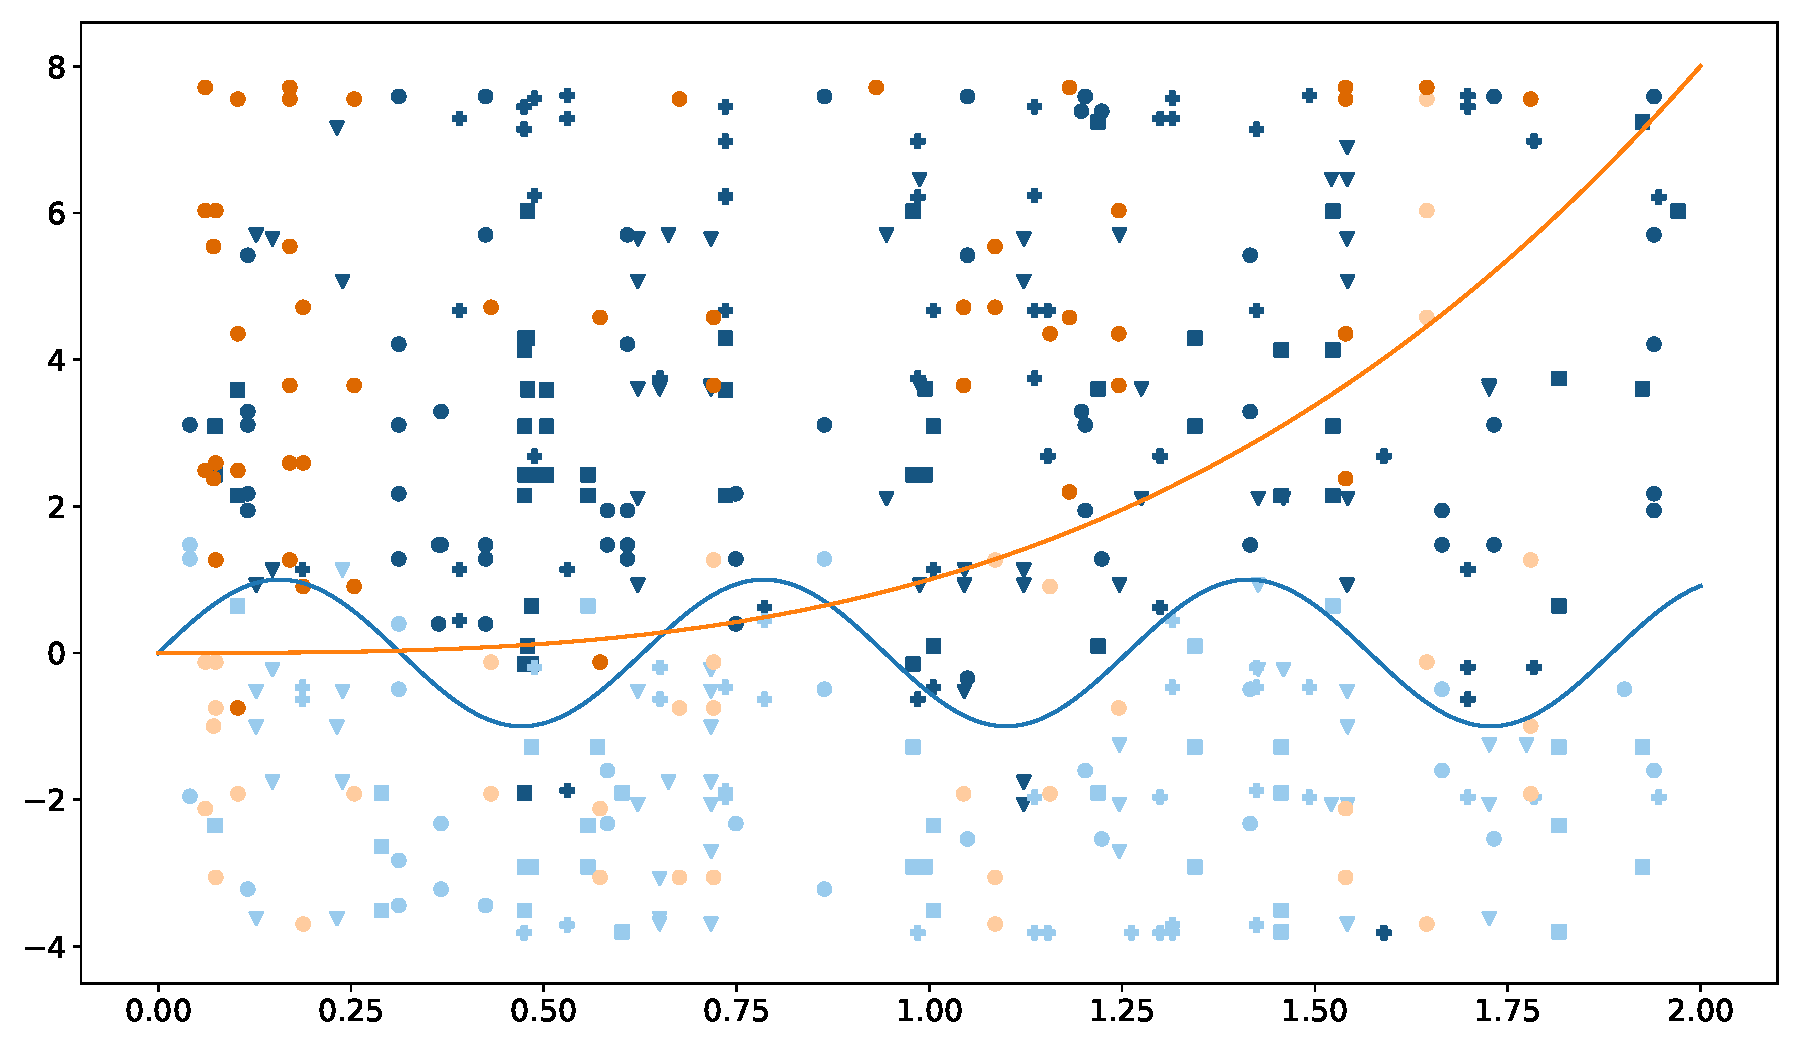
\includegraphics[width=\textwidth]{Chapter6/IGPL2022/clasClusters__2.pdf}
            \caption{\fdata{clasClusters2}.}
            %\label{clasClusters0}
      \end{subfigure}
      \end{figure}

\end{frame}



\begin{frame}
      \frametitle{Experimentos Sintéticos: Resultados}

      \begin{table}
            % \caption{\acrshort{mae} scores for synthetic regression problems and F1 scores for synthetic classification ones. In bold we highlight the best models of each group: L1, L2 or LS-\acrshort{svms}.}
            % \label{tab:full_synthetic}
            \centering
            \scalebox{.65}{
            \begin{tabular}{lccc|ccc}
                \toprule
                {} &  \fhead{\fdata{regClusters0}} &  \fhead{\fdata{regClusters1}} &  \fhead{\fdata{regClusters2}} &  \fhead{\fdata{clasClusters0}} &  \fhead{\fdata{clasClusters1}} &  \fhead{\fdata{clasClusters2}} \\
                \midrule
                & \fheadmulti{3}{MAE} & \fheadmulti{3}{F1} \\
                \midrule
                \fmod{CTL-L1}               &            0.989 &            0.512 &            0.541                 &             0.901 &             0.912 &             0.904 \\
                \fmod{ITL-L1}               &            0.221 &            0.212 &            0.159                 &             0.922 &             0.923 &             0.910 \\
                \fmod{MTL-L1}         &            0.213 &            0.176 &            0.135           &             \fmaxn{0.924} &             0.925 &             0.914 \\
                \fmod{cvxGLMTL-L1}       &            0.212 &            0.173 &            0.138         &             0.920 &             0.926 &             0.912 \\
                \fmod{AdapGLMTL-L1}   &            \fmaxn{0.152} &            \fmaxn{0.116} &            \fmaxn{0.107}     &             \fmaxn{0.924} &             \fmaxn{0.929} &             \fmaxn{0.916} \\
                \midrule
                \fmod{CTL-L2}             &            0.990 &            0.642 &            0.768               &             0.904 &             0.912 &             0.906 \\
                \fmod{ITL-L2}             &            0.213 &            0.201 &            0.154               &             \fmaxn{0.928} &             0.928 &             0.910 \\
                \fmod{MTL-L2}       &            0.209 &            0.168 &            0.131         &             0.925 &             0.927 &             0.913 \\
                \fmod{cvxGLMTL-L2}     &            0.204 &            0.169 &            0.131       &             0.921 &             0.923 &             \fmaxn{0.915} \\
                \fmod{AdapGLMTL-L2} &            \fmaxn{0.141} &            \fmaxn{0.115} &            \fmaxn{0.103}   &             0.924 &             \fmaxn{0.929} &             \fmaxn{0.915} \\
                \midrule
                \fmod{CTL-LS}             &            0.989 &            0.642 &            0.766               &             0.895 &             0.908 &             0.894 \\
                \fmod{ITL-LS}             &            0.212 &            0.209 &            0.149               &             0.914 &             0.915 &             0.904 \\
                \fmod{MTL-LS}       &            0.206 &            0.167 &            0.131         &             0.917 &             0.917 &             \fmaxn{0.905} \\
                \fmod{cvxGLMTL-LS}     &            0.207 &            0.169 &            0.132       &             0.919 &             \fmaxn{0.921} &             0.897 \\
                \fmod{AdapGLMTL-LS} &            \fmaxn{0.136} &            \fmaxn{0.115} &            \fmaxn{0.106}   &             \fmaxn{0.920} &             \fmaxn{0.921} &             0.901 \\
                \bottomrule
            \end{tabular}
            }
        \end{table}

\end{frame}

\begin{frame}
      \frametitle{Experimentos Sintéticos: Resultados}
      
      \centering
      \begin{figure}
            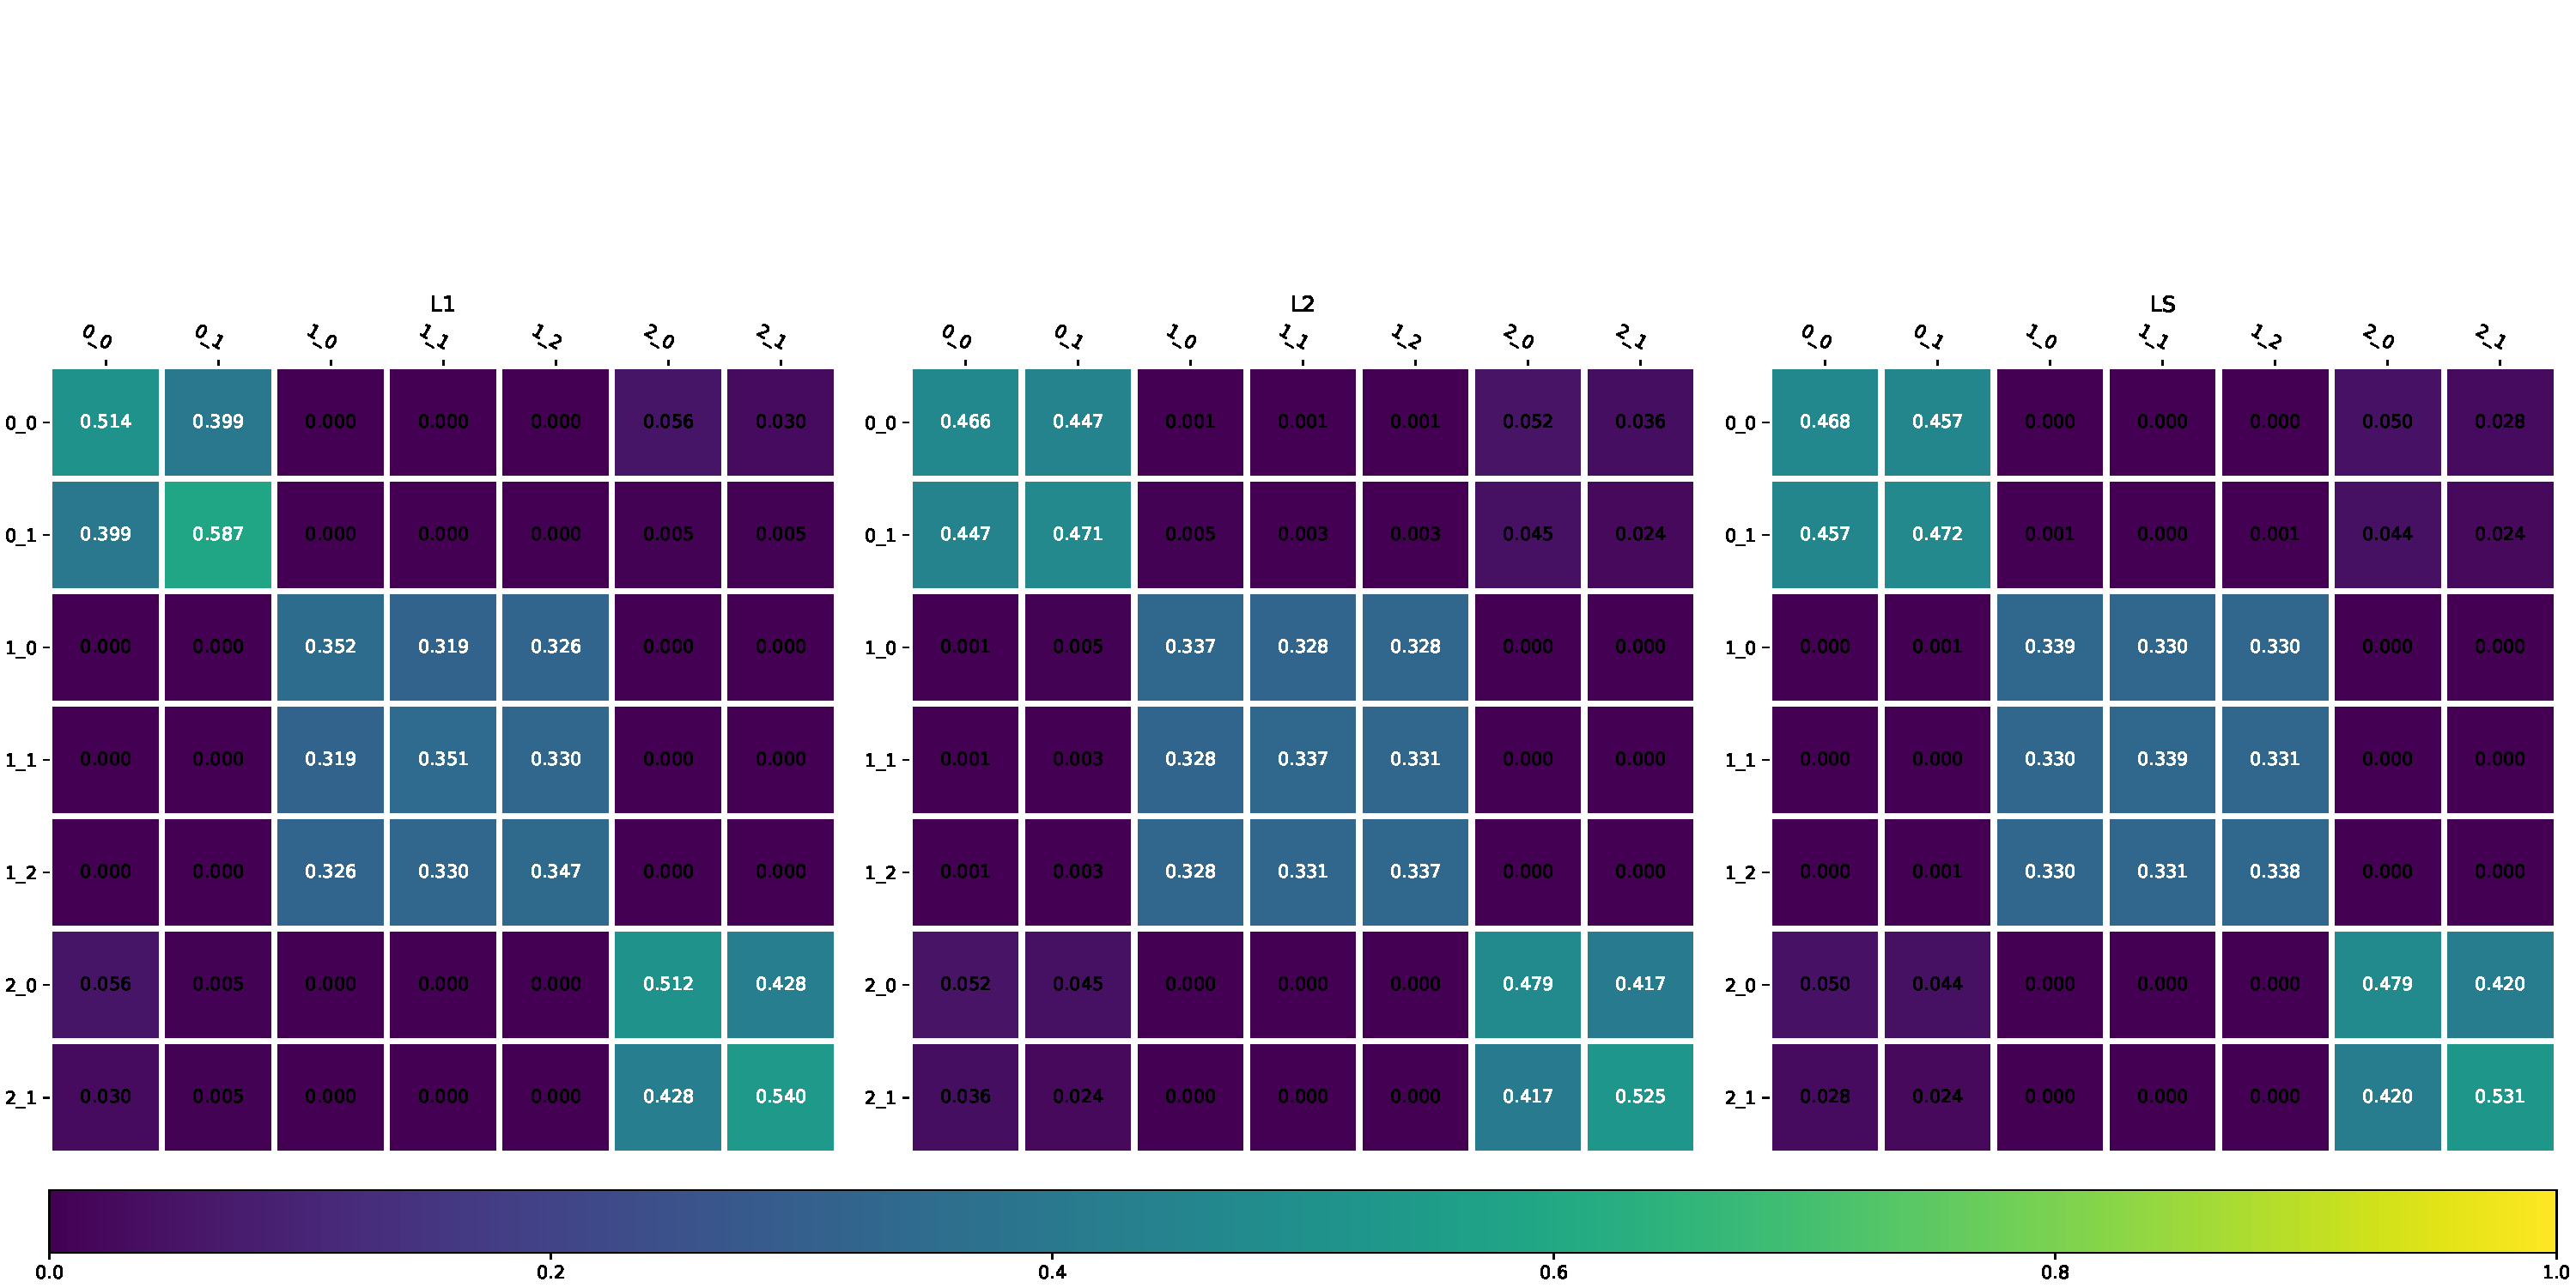
\includegraphics[width=.85\textwidth]{Chapter6/IGPL2022/adjMatrix_all__regClusters_0.pdf}
            \caption{Prueba}
      \end{figure}

\end{frame}

\begin{frame}
      \frametitle{Experimentos Sintéticos: Resultados}
      
      \centering
      \begin{figure}
            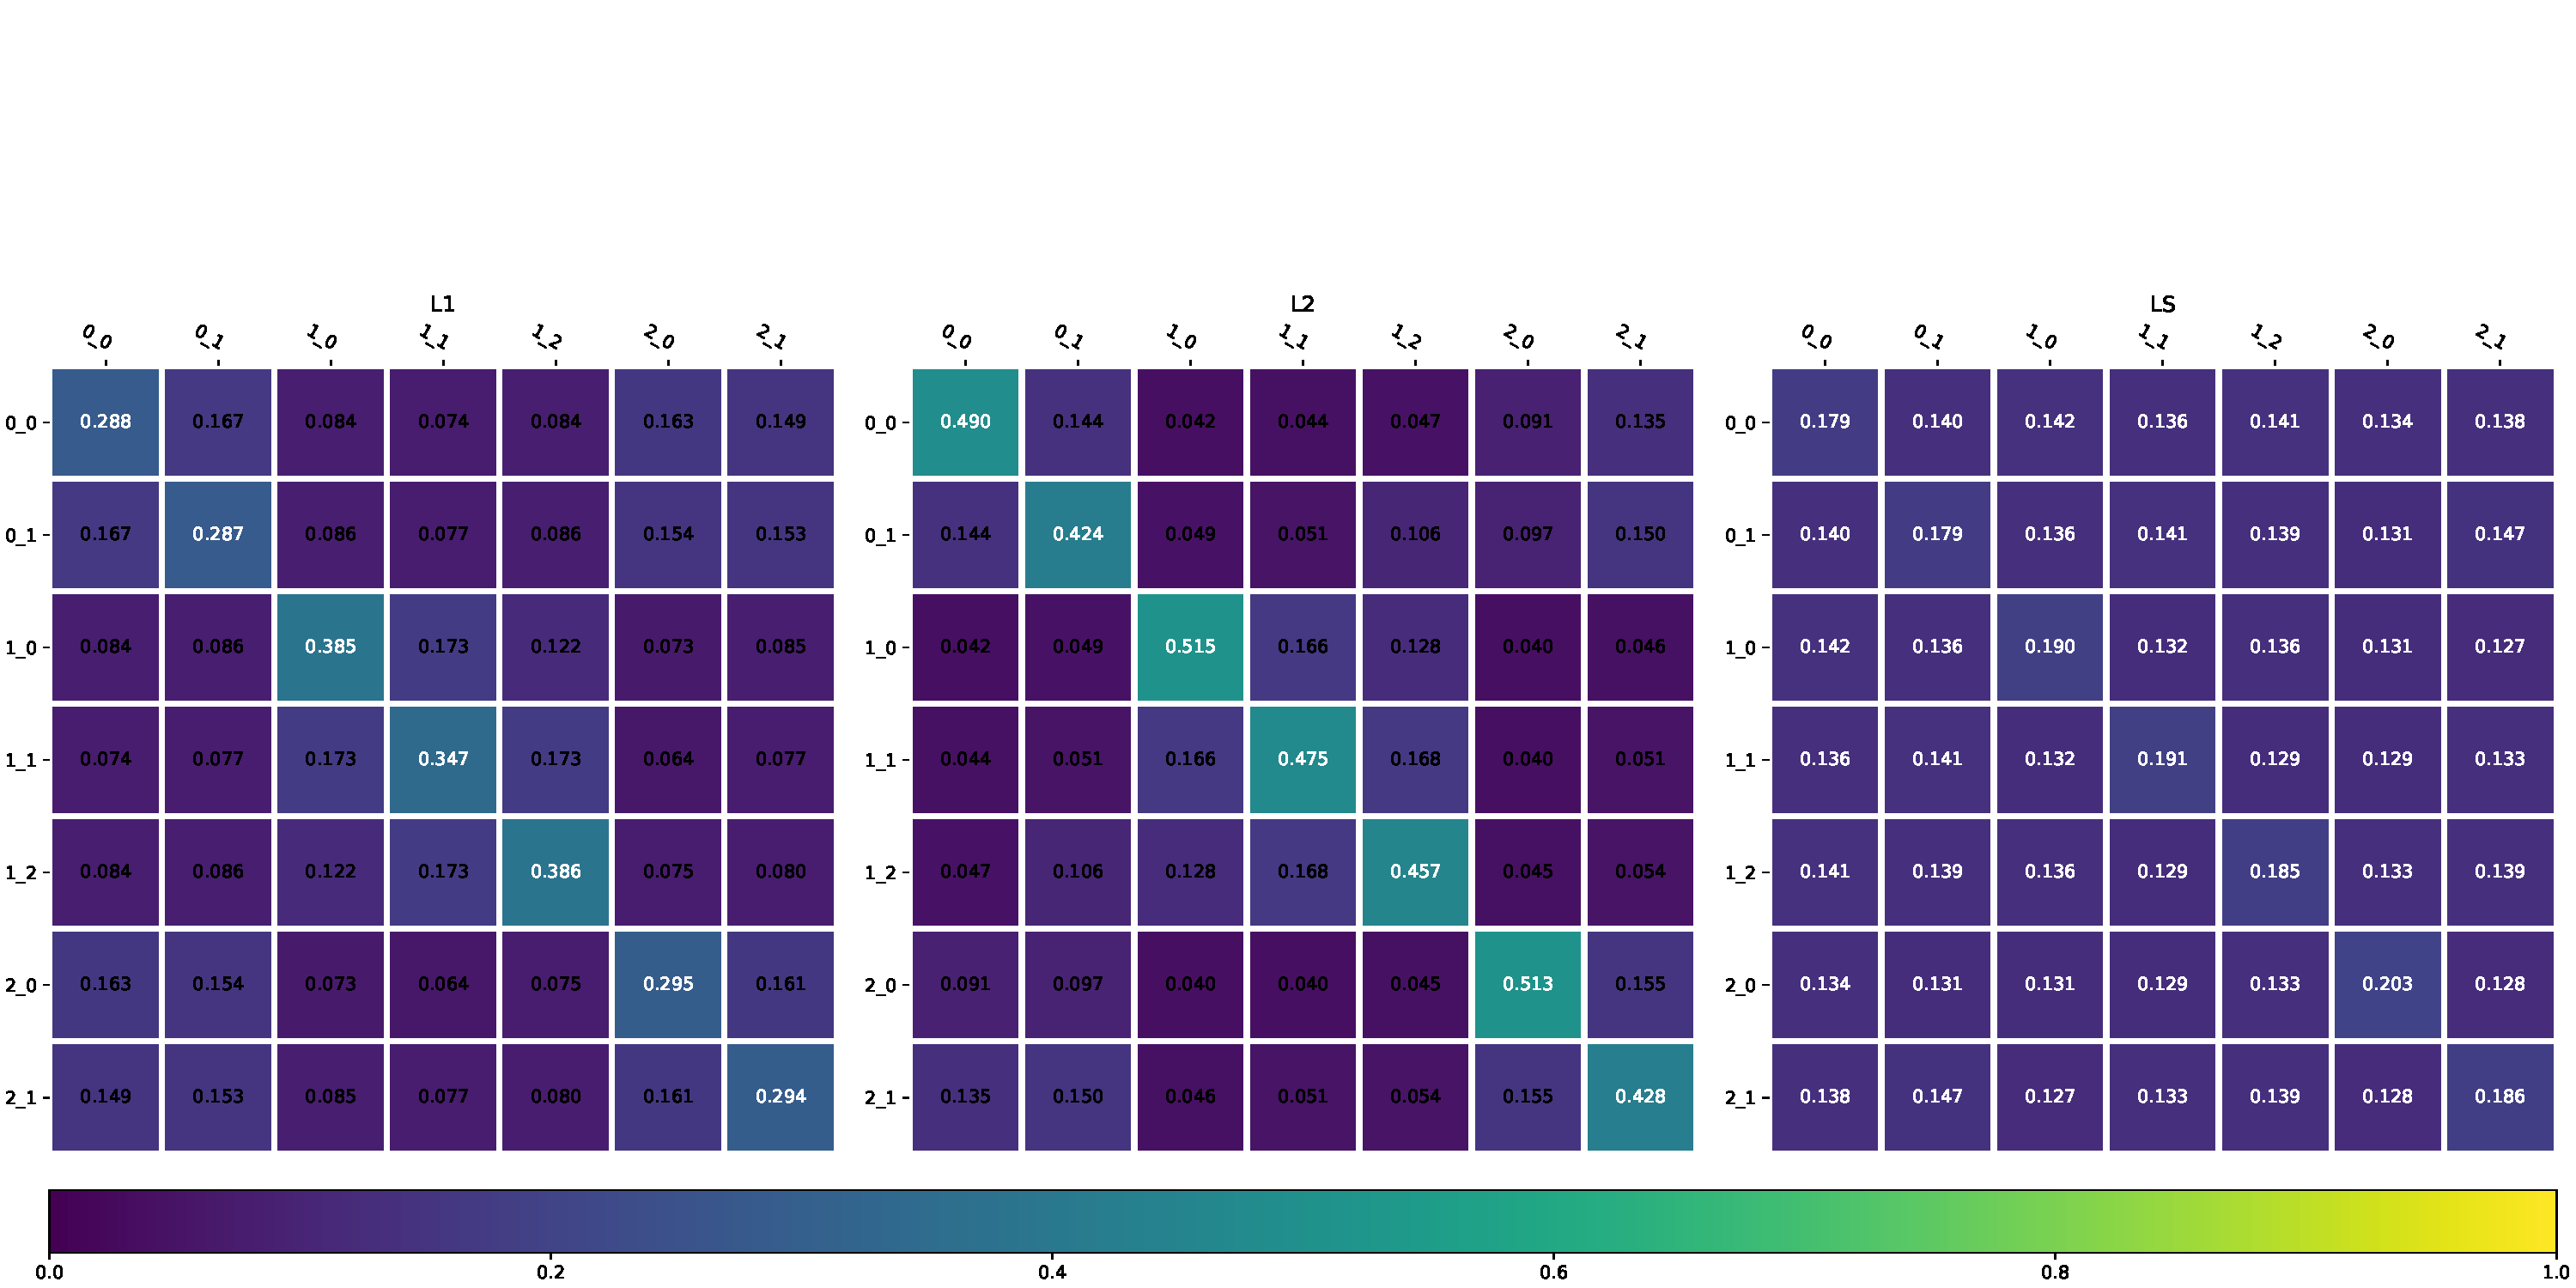
\includegraphics[width=.85\textwidth]{Chapter6/IGPL2022/adjMatrix_all__clasClusters_0.pdf}
            \caption{Prueba}
      \end{figure}

\end{frame}


\section{Summary}

\begin{frame}
\frametitle{Good Luck!}
\begin{itemize}
\item Enough for an introduction! You should know enough by now
\end{itemize}
\end{frame}

\backmatter
\end{document}
